
\chapter{RESULTADOS}

Este capitulo expõe os resultados obtidos através da execução dos testes de unidade no aplicativo MIP, como o número de testes desenvolvidos durante o desenvolvimento do trabalho é extenso foram escolhidas as principais classes do pacote \textit{Entity} (\textit{Field.java e Survey.java}), e as principais classes do pacote \textit{Service} (\textit{FieldService.java e SurveyService.java}). para serem analisadas profundamente. 


\section{APURAÇÃO DOS TESTES PACOTE ENTITY}

O pacote \textit{Entity} é responsável por armazenar as classes que realizam o mapeamento objeto-relacional, e nele é definida as principais regras de negócio do sistema. O pacote é composto por 5 sub pacotes sendo eles: 

\begin{itemize}

\item[1]Pacote \textit{base}: Armazenas as classes que define a estrutura básica do sistema, as classes que definem regiões (\textit{Region.java}), cidades (\textit{City.java}), estados (\textit{State.java}) e macrorregiões (\textit{MacroRegion.java}), assim como as que definem supervisores (\textit{Supervisor.java}) e agricultor (\textit{Farmer.java}). Todos esses dados compõem um registro (\textit{Field.java}) que estabelece uma ligação entre localização, supervisores e agricultor. Além disso o pacote contém mais duas superclasses, \textit{AuditingPersistenceEntity.java} responsável por armazenar metadados dos objetos, e \textit{Person.java} responsável por definir os atributos básicos de uma pessoa.  

\item[2]Pacote mid: Armazena as classes que definem a estrutura básica para coleta e análise de esporos de ferrugem asiática e doenças que afetam a lavoura. A classe \textit{AsiaticRustTypesLeafInspection.java} contém os tipos de lesões causadas pela ferrugem em plantas, a classe \textit{AsiaticRustTypesSporeCollector.java} contém os tipos de análise que podem ser retiradas do coletor de esporos, a classe \textit{BladeReadingResponsibleEntity.java} armazena a entidade responsável pela leitura de laminas de esporos, classe \textit{BladeReadingResponsiblePerson.java} é responsável por armazenar a pessoa responsável pela leitura de esporos, \textit{MIDSampleSporeCollectorOccurrence.java} trata os dados da amostra de esporos coletada, \textit{MIDSampleLeafInspectionOccurrence.java} trata os dados da inspeção das folhas coletada, \textit{MIDSampleFungicideApplicationOccurrence.java} trata os dados da aplicação de fungicida contra a ferrugem. A classe principal deste pacote é a \textit{MIDRustSample.java} pois é nela onde são armazenados todos os registros de aplicação de fungicida, de coleta de folhas, de coleta de sopros e os responsáveis pelas análises. 

\item[3]Pacote mip: Armazena as classes que definem a estrutura básica para coleta e análise de pragas que atingem a lavoura.  A classe \textit{Pest.java} registra os tipos de pragas que podem atingir uma lavoura, \textit{PestDisease.java} armazena as doenças causadas por pragas, \textit{PestSize.java} é responsável pelo armazenamento do tamanho das pragas. \textit{GrowthPhase.java} registra a fase de crescimento em que a praga foi encontrada, \textit{PestNaturalPredator.java} armazena os predadores naturais das pragas, \textit{MIPSamplePestOccurrence.java} registra a ocorrência de pragas em uma lavoura, \textit{MIPSamplePestDiseaseOccurrence.java} registra a ocorrência de doenças causadas por pragas em uma lavoura, \textit{MIPSampleNaturalPredatorOccurrence.java} registra a ocorrência de predadores naturais na lavoura. A classe principal deste pacote é a \textit{MIPSample.java} ela é responsável por armazenar os dados de pragas, doenças causadas por pragas e predadores naturais que atingem uma lavoura.

\item[4]Pacote \textit{pulverisation}: Armazena as classes que definem a estrutura básica para a atividade de pulverização de uma lavoura. As classes \textit{ProductUnit.java} e \textit{Product.java} são responsáveis por tratar dos produtos que serão utilizados durante a pulverização, definem unidade de medida do produto e características do produto como nome e dose respectivamente. As classes \textit{TargetCategory.java} e \textit{Target.java} definem a categoria alvo do pesticida e qual praga ele combate respectivamente. A classe \textit{PulverisationOperationOccurrence.java} define uma ocorrência de pulverização.  A principal classe deste pacote é a \textit{PulverisationOperation.java} esta contém os dados referente a todas as pulverizações que foram realizadas. 

\item[5]Pacote \textit{survey}: Armazena as classes que definem a estrutura básica para realizar uma pesquisa de campo através dos dados coletados com o manejo integrado de pragas e com o manejo integrado de doenças. A classe \textit{DateData.java} armazena os dados de uma colheita como data de semeadura e data da colheita, a classe \textit{SizeData.java} contém os dados referente a área da colheita, a classe \textit{LocationData.java} contém dados referente a localização da colheita, a classe \textit{ProductivityData.java} contém dados referente a produtividade de uma colheita, a classe \textit{QuestionData.java} registra dados específicos referente a plantação, se a plantação é resistente a ferrugem por exemplo, a classe \textit{Harvest.java} e responsável por registrar dados referente a colheita como o início e o fim da colheita. A principal classe deste pacote é a \textit{Survey.java} ela é responsável por armazenar todos os dados referente a uma pesquisa da produção da lavoura de um produtor.

\end{itemize}{}

\subsection{RESULTADO DOS TESTES CLASSE FIELD.JAVA}

Como já foi ressaltado anteriormente uma das principais classes do sistema é a \textit{Field.java}, a FIGURA \ref{diagrmaTestField} apresenta o diagrama de classes que expressa a classe \textit{Field.java}, e as demais classes que a compõem assim como a classe responsável por testá-la, a classe FieldTest.java. Também é possível analisar no diagrama os atributos e métodos que pertence à classe \textit{Field}, assim como os métodos e atributos da classe de teste \textit{FieldTest}.

\begin{figure}[H]
	\centering
	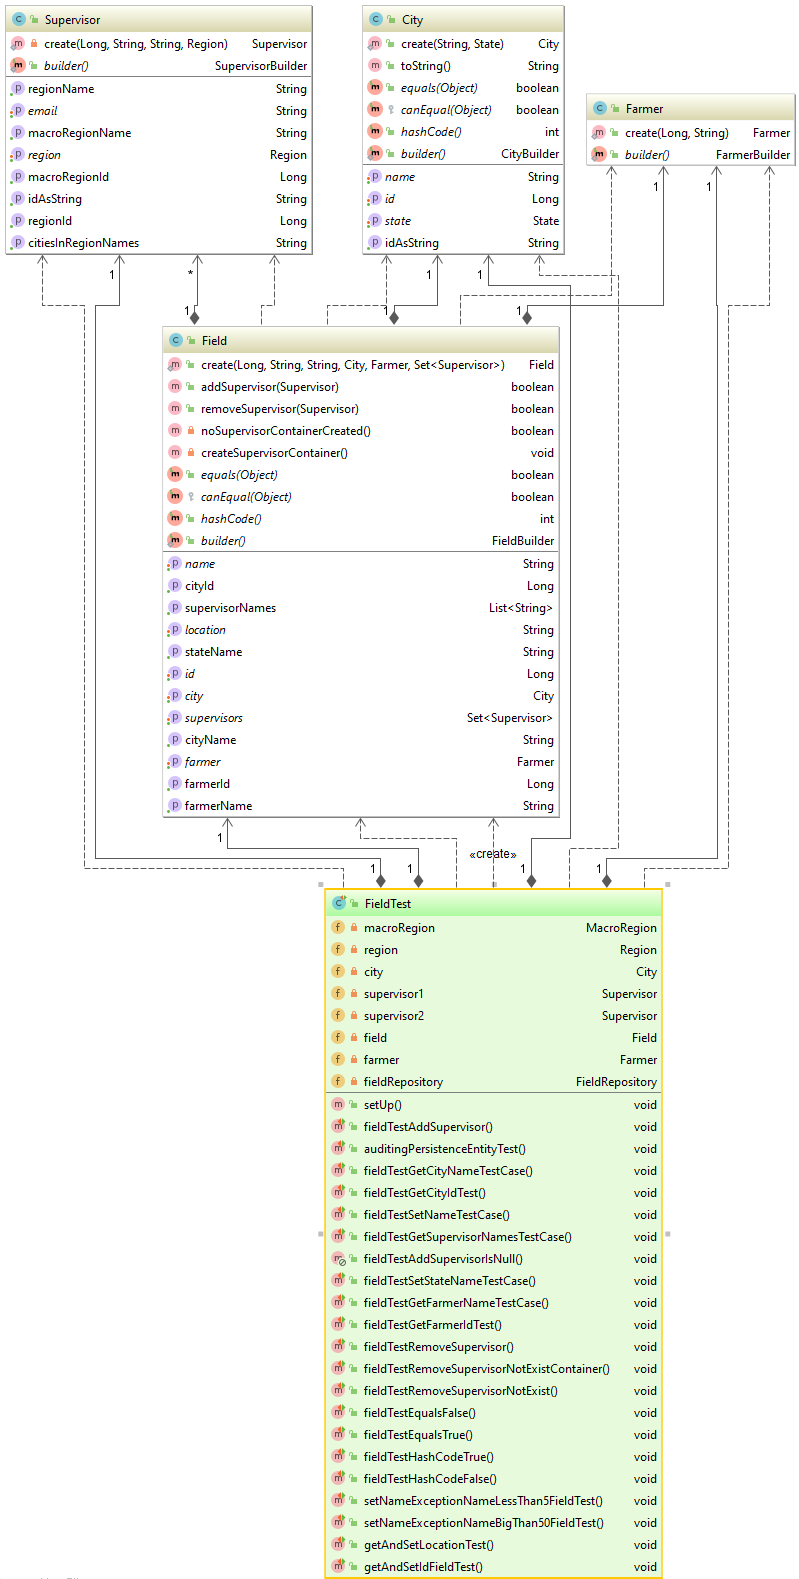
\includegraphics[scale=0.58]{dados/figuras/PackagebaseTestField.png}
	\caption{Diagram de Classes Field e FieldTest.}
	\label{diagrmaTestField}
\end{figure}

A classe de teste apresentada na FIGURA \ref{diagrmaTestField} possui vinte e um métodos de teste e um método de apoio aos testes denominado \textit{“setUp”}, o objetivo dos testes é exercitar a classe \textit{Field} até que todos as variáveis, entradas e saídas de dados sejam executados pelo menos uma vez. Como a classe \textit{Field} é composta por outras classes se faz necessário a instanciação de outras classes como \textit{Supervisor}, \textit{Farmer}, \textit{City} e outras para a execução completa dos testes. Como a classe se trata de uma entidade que será persistida em um banco de dados, ela possui certas regras de negócio que serão ativadas somente no momento de gravar os dados no banco, sendo assim foi preciso criar uma referência para a interface \textit{FieldRepository}, classe responsável por realizar a persistência dos dados no banco. Como o objetivo deste trabalho é cobrir o sistema com testes unitários e testes que integram classes entidades com o banco de dados ou comunicação com \textit{APIs} são testes de integração foi utilizado um\textit{ “Mock”} para simular o comportamento do repositório.

A FIGURA \ref{field1} apresenta a declaração da classe de testes, os atributos utilizados para desenvolver os testes e o método\textit{ “setUp”} utilizado para preparar o ambiente para os testes.


O trecho de código da FIGURA \ref{field1} apresenta as seguintes funcionalidades:





\begin{itemize}

\item Na linha 1 é utilizada a anotação \textit{@SpringBootTest} que prepara um contexto \textit{Spring} e inclui a possibilidade de iniciar um container em um porta default ou configurada pelo usuário. O que não é necessário para o tipo de teste executado nesta classe; 

 \item Na linha 2 é utilizada a anotação \textit{@FixMethodOrder} que permite definir uma ordem de execução dos testes, neste casso foi definida a ordem \textit{“NAME\_ASCENDING"} que faz a execução dos testes de acordo com o nome de maneira ascendente;

 \item Linha 3 a classe \textit{FieldTest} é aberta;

 \item Da linha 5 a 10 há a declaração dos objetos que serão utilizadas nos testes;
 
  \item Na linha 12 um objeto do tipo \textit{FieldRepositorio} e declarado e instanciado como um objeto \textit{mock}.

 \item Na linha 15 é utilizado a anotação \textit{@Before}, esta anotação determina que, sempre antes da execução de um teste o método \textit{“setUp”} deve ser executado primeiro.

 \item O método \textit{“setUp”} que tem sua declaração na linha 15 e vai até a linha 30 é responsável por realizar a construção dos objetos declarados nas linhas 5 a 10.


\end{itemize}{}



A FIGURA \ref{field1} apresenta os casos de testes criados para a classe \textit{Field}. 


A ideia geral na elaboração dos testes é a de cobrir cada atribuição de dados, as entrada e saída de dados da classe \textit{Field}, buscando a cobertura de 100\% das linhas métodos e atributo da classe. Os resultados obtidos da execução dos testes foram listados a seguir:

Método de teste \textit{“fieldTestAddSupervisor()”} linhas 32 a 36 figura \ref{field1}: Este método é responsável por testar se um objeto do tipo\textit{ “supervisor”} é adicionado ao objeto testado através do método de entrada \textit{“field.addSupervisor(Supervisor supervisor)”}.  Neste teste a entrada é um objeto do tipo \textit{“Supervisor” }e a saída do método é uma variável do tipo \textit{“boolean”}(verdadeiro ou falso).  As entradas foram criadas nas linhas 24 e 26 e fornecidas como entradas ao método testado nas linhas 34 e 35 respectivamente. A saída é um \textit{“TRUE”} já que os objetos passados são adicionados a classe\textit{ “Field”}. 



Método de teste\textit{ “auditingPersistenceEntityTest()”} linhas 38 a 47 figura \ref{field1}: Este método é responsável por testar os atributos criados na superclasse\textit{ “auditingPersistenceEntity”}, como uma superclasse não pode ser testada os métodos e atributos dela devem ser testados em uma das subclasses.  A classe é composta por dois atributos do tipo \textit{long “LastModified”} e \textit{“CreatedAt”,} O objetivo deste teste é de atribuir valor as variáveis e verificar se os valores atribuídos são recuperados corretamente. As entradas foram criadas nas linhas 40 e 41 e atribuídas ao objeto testado nas linhas 43 e 44 respectivamente. Posteriormente nas linhas 45 e 46 é feita a confirmação das saídas contendo os valores 11 e 12 do tipo \textit{“long”.}

Método de teste \textit{“fieldTestGetCityNameTestCase ()”} linhas 49 a 52 figura \ref{field1}: Este caso de teste verifica se um nome atribuído a uma cidade é recuperado pelo método \textit{“field.getCityName()”.} A entrada é uma \textit{String} de caracteres, e a saída deve ser uma \textit{String} de caracteres formatados com a primeira letra de cada palavra maiúscula.  O objeto do tipo \textit{“city” }é criado na linha 19 o atribuído nome é definido como “NOvA FAtimA” em seguida o objeto\textit{ “city”} é atribuído ao objeto\textit{ “Field” }na linha 28 /29. Já no teste o valor e recuperado é o retorno é “Nova Fatima”.


\begin{figure}[H]
	\centering  
	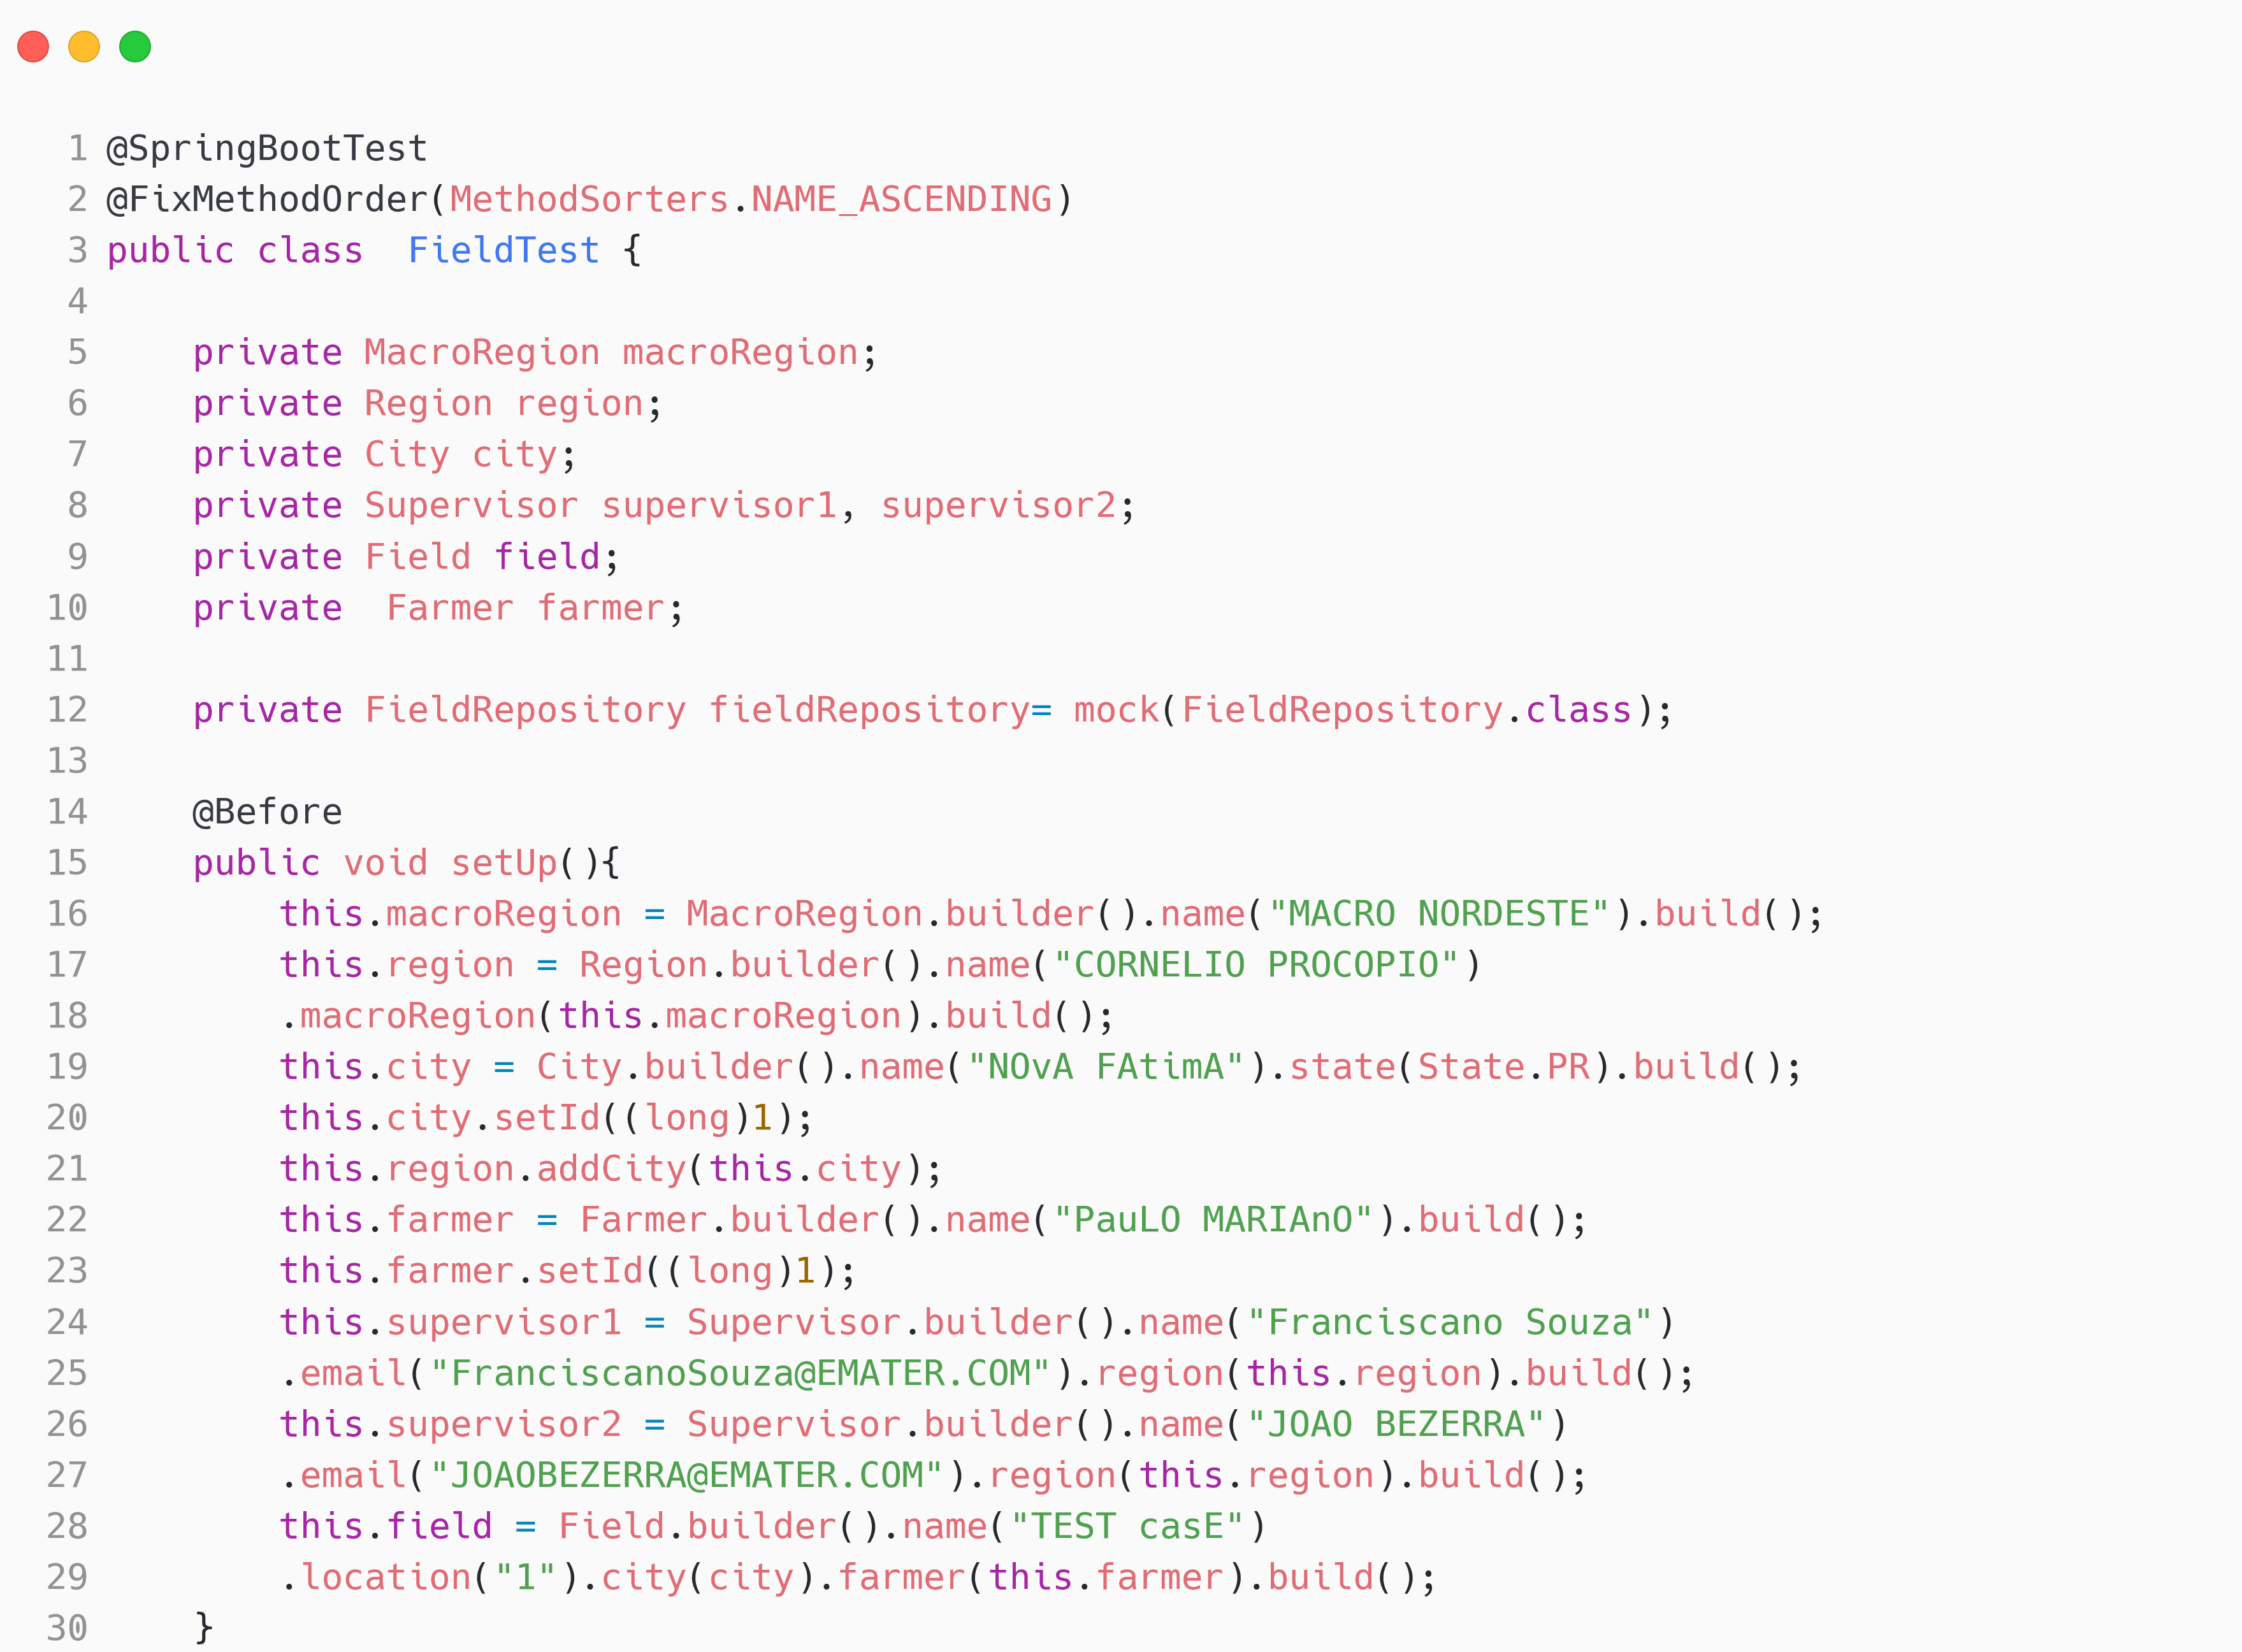
\includegraphics[scale=0.18]{dados/figuras/buildTestField.png}
\end{figure}

\begin{figure}[H]
	\centering
	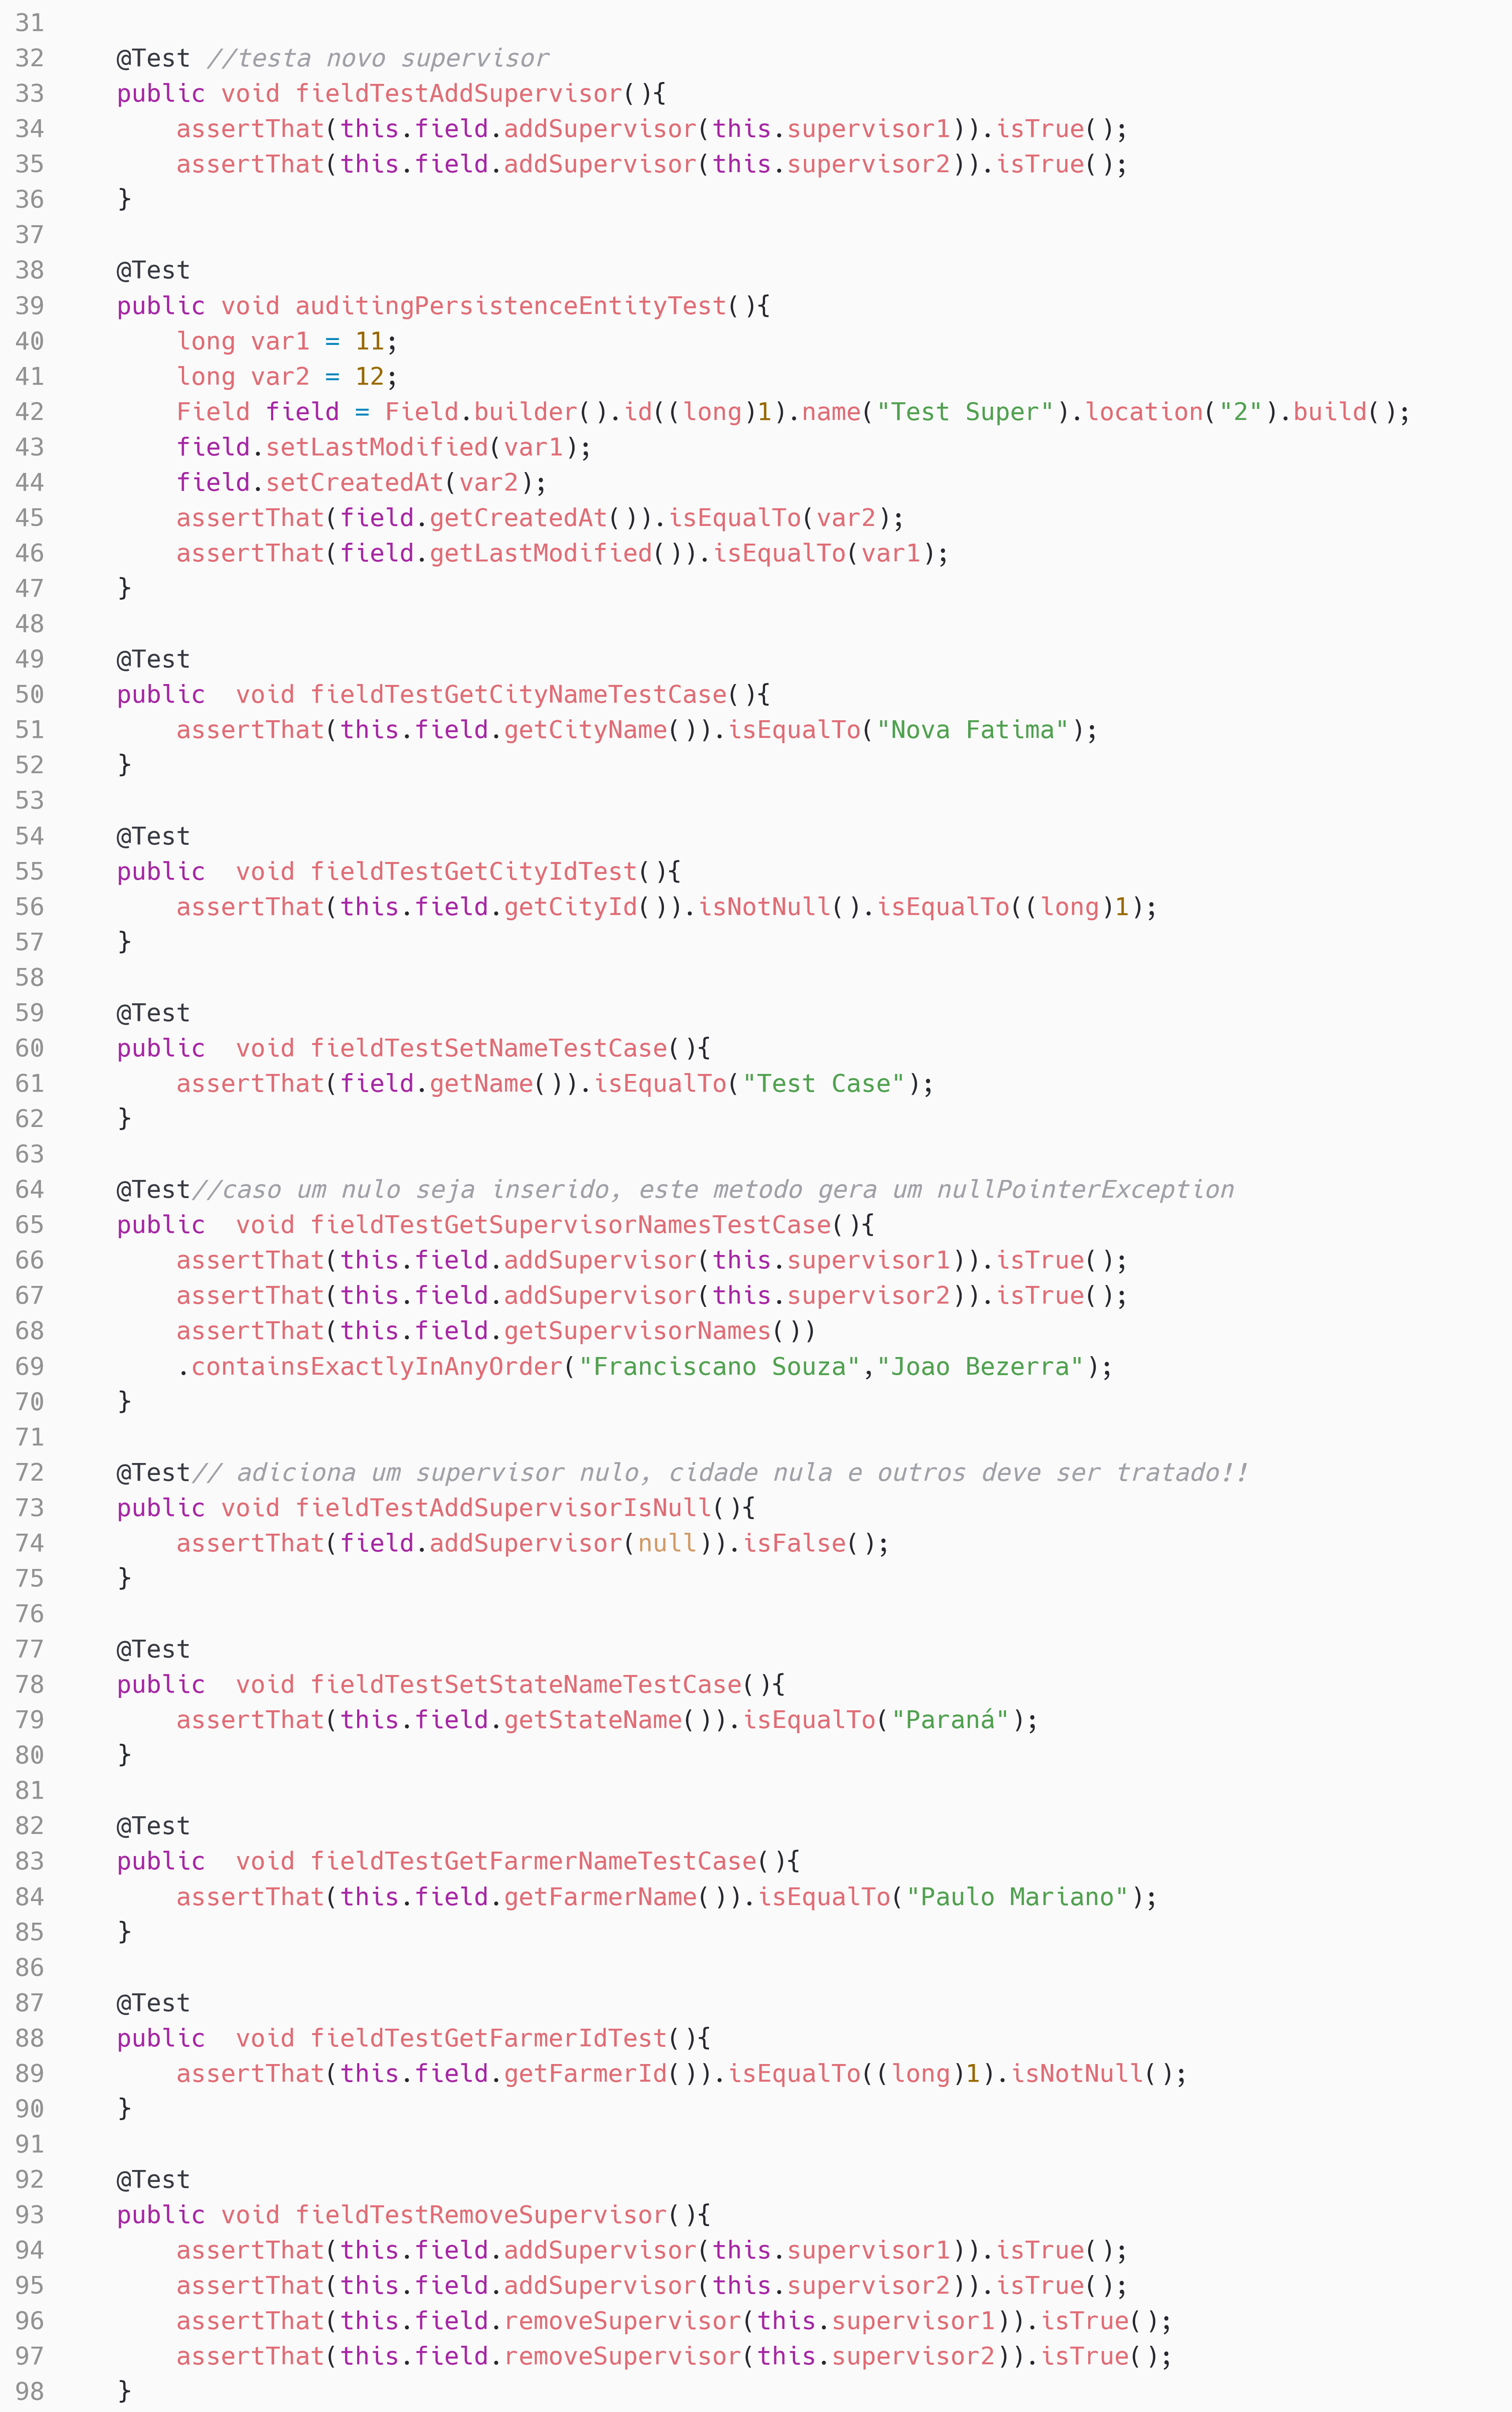
\includegraphics[scale=0.18]{dados/figuras/carbonField1.png}
\end{figure}

\begin{figure}[H]
	\centering
	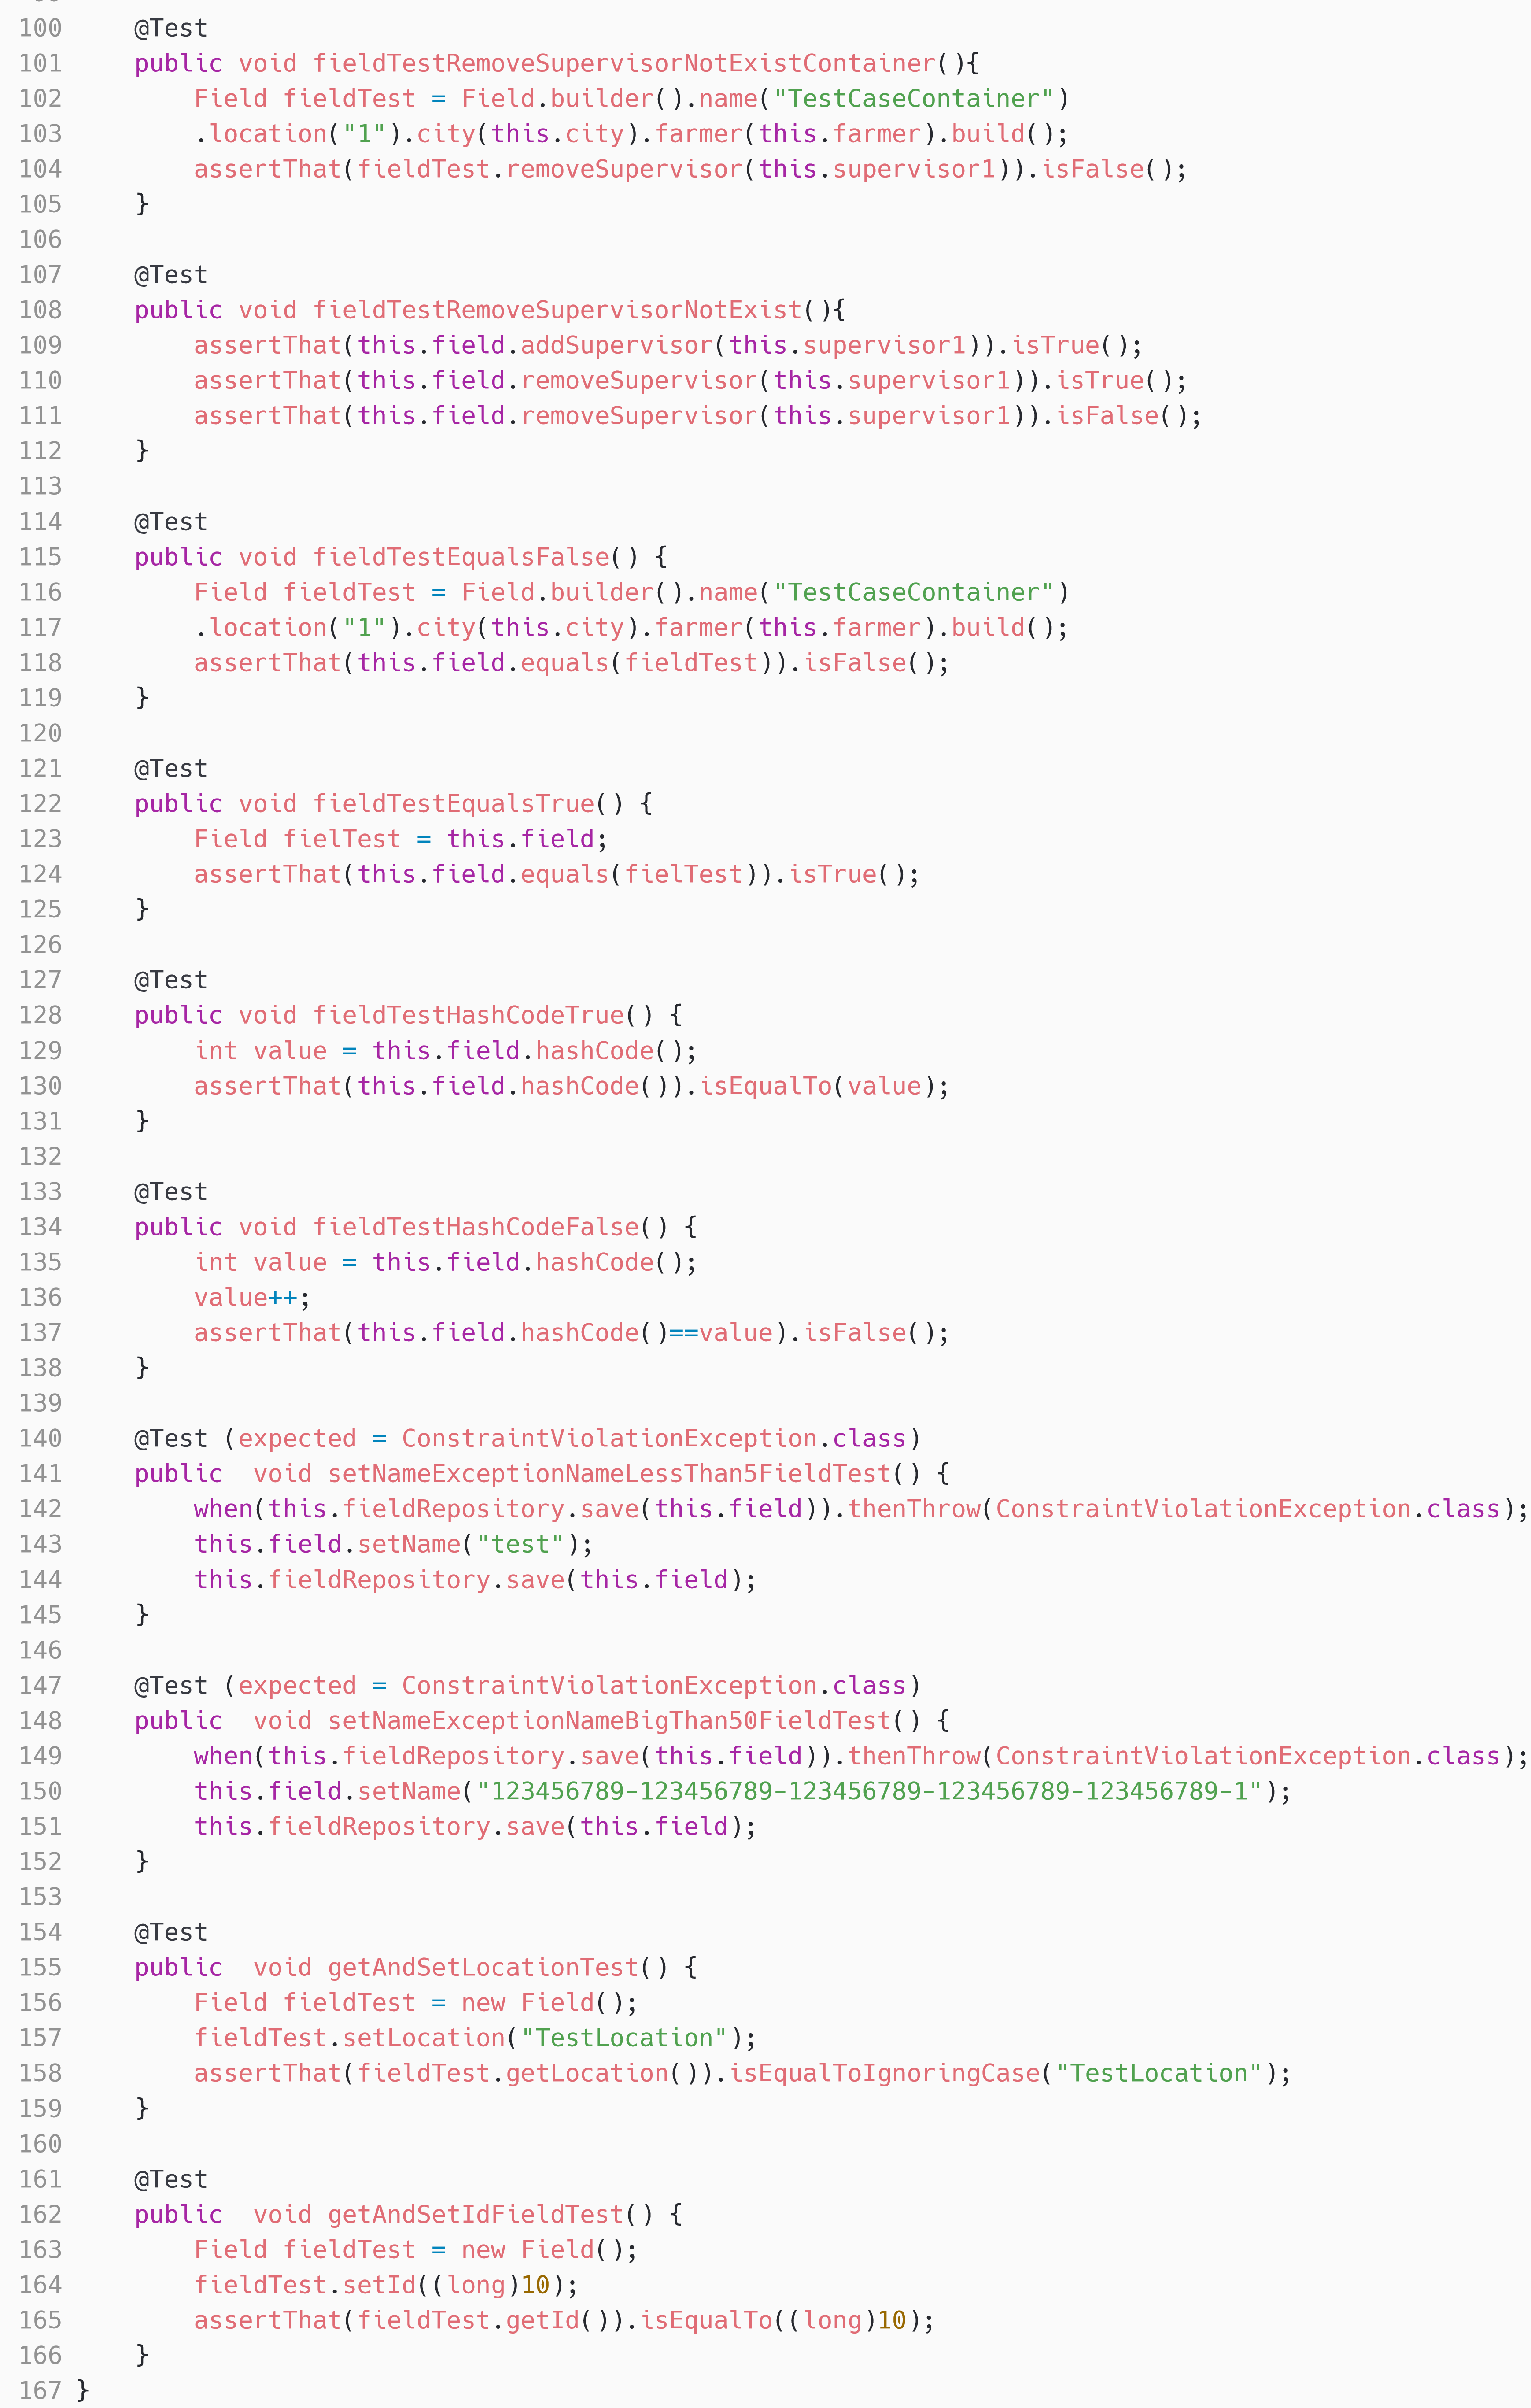
\includegraphics[scale=0.17]{dados/figuras/carbonField2.png}
	\caption{Classe de teste FieldTest.java.}
	\label{field1}
\end{figure}






Método de teste\textit{ “fieldTestGetSupervisorNamesTestCase()”} linhas 64 a 70 figura \ref{field1}: Este caso de teste verifica se o método\textit{ “Field.getSupervisorNames ()”} recupera os nomes de todos os supervisores adicionados ao objeto \textit{“Field”.} Os supervisores são criados nas linhas 24 a 27 e são adicionados a\textit{ “Field”} nas linhas 66 e 67. A entrada é composta por dois supervisores de nomes diferentes ("Franciscano Souza" e "Joao Bezerra"). O retorno do método testado consiste em uma lista do tipo \textit{“String”}, o teste verifica se a lista contem em qualquer ordem os elementos os elementos inseridos, o retorno é ("Franciscano Souza" e "Joao Bezerra");

Método de teste\textit{ “fieldTestAddSupervisorIsNull()”} linhas 72 a 75 figura \ref{field1}: Este caso de teste consiste em inserir um supervisor como\textit{ “null”}, caso o nulo seja inserido gera uma inconsistência pois outros métodos de consulta podem falhar. A entrada é um\textit{ “null”} linha 74, e o retorno esperado é um \textit{“FALSE”,} pois, a inserção não deve ser realizada, mas o retorno é um\textit{ “TRUE”} confirmando à inserção de um nulo como um supervisor. Esta inserção pode gerar uma inconsistência em consultas futuras.

Método de teste\textit{ “fieldTestSetStateNameTestCase ()”} linhas 64 a 70 figura \ref{field1}: Este teste consiste em recuperar o nome do estado a qual a cidade pertence. A Entrada consiste em um objeto do tipo \textit{“Estate.PR”} linha 19. O retorno esperado é uma \textit{string} de caracteres contendo “Paraná”. O retorno do método testado é uma \textit{string} contendo “Paraná”   

Método de teste \textit{“fieldTestGetFarmerNameTestCase ()”} linhas 82 a 85 figura \ref{field1}: Este meto busca o nome do agricultor atribuído ao objeto\textit{ “Field”}. A entrada consiste em um objeto do tipo\textit{ “Farme” }com o atributo nome definido como “PauLO MARIAnO” linha 22. O retorno do método testado deve ser uma \textit{string} contendo o nome do agricultor formatado com a primeira letra de cada palavra maiúscula. O retorno do teste linha 84 é uma \textit{string} que contem “Paulo Mariano”.


Método de teste\textit{ “fieldTestGetFarmerIdTest ()”} linhas 87 a 90 figura \ref{field1}: Este método consiste em recuperar o atribuo identificador de agricultor a entrada é feita na linha 23 sendo o valor (\textit{long} 1). O retorno do método testado deve ser um \textit{long} contendo o identificador único do agricultor. O retorno do meto é um tipo \textit{long} contendo o valor 1. 


Método de teste \textit{“fieldTestRemoveSupervisor ()”} linhas 92 a 98 figura \ref{field1}: Este teste consiste em atribuir novos supervisores a um objeto\textit{ “Field”} e em seguida remove-los. A entrada consiste em dois supervisores linhas 94 e 95. A saída consiste em um\textit{ “boolean”} para cada remoção\textit{, “TRUE”} caso o supervisor seja removido, e\textit{ “FALSE”} caso o supervisor não seja removido.  A sida nesse teste é\textit{ “TRUE”} para as duas execuções pois os dois supervisores enviados para remoção foram encontrados.

Método de teste\textit{ “fieldTestRemoveSupervisorNotExistContainer ()”} linhas 100 a 105 figura \ref{field1}: Este caso de teste consiste em tentar remover um supervisor de um objeto \textit{“Field” }sem que não haja um container do tipo supervisor criado em\textit{ “Field”}. A entrada consiste em um supervisor não pertencente ao objeto \textit{“FieldTest”} criado na linha 102. A saída nesse caso de teste é um\textit{ “FALSE”} pois ainda não foi inserido nenhum supervisor a \textit{“FieldTest”}.
 
Método de teste \textit{“fieldTestRemoveSupervisorNotExist()” }linhas 107 a 112 figura \ref{field1}: Este método consiste em testar a remoção de um supervisor que já foi removido anteriormente. A entrada consiste em um supervisor linhas 109. A saída consiste em \textit{“TRUE”} caso os objetos sejam removidos com sucesso, saída apresentada na linha 110 ou \textit{“FALSE”} caso o supervisor já não exista mais em\textit{ “Field” }saída apresentada na linha 111.

Método de teste\textit{ “fieldTestEqualsFalse()”} linhas 114 a 119 figura \ref{field1}: Este método de teste consiste em comparar dois objetos do tipo\textit{ “Field”} caso eles sejam iguais o retorno é um\textit{ “boolean” “TRUE”} caso sejam diferentes o retorno é um\textit{ “FALSE”}. A entrada consiste em dois objetos do tipo\textit{ “Field”}, o primeiro objeto é criado nas linhas 28 e 29, o segundo objeto é criado nas linhas 116 e 117. A saída é um \textit{“FALSE” }pois os objetos comparados são diferentes.

Método de teste \textit{“fieldTestEqualsTrue()” }linhas 121 a 125 figura \ref{field1}: Este método de teste consiste em comparar dois objetos do tipo\textit{ “Field”} caso eles sejam iguais o retorno é um \textit{“boolean” “TRUE”} caso sejam diferentes o retorno é um\textit{ “FALSE”}. A entrada consiste em dois objetos do tipo \textit{“Field”,} o primeiro objeto é criado nas linhas 28 e 29, o segundo objeto é criado nas linhas 116 e 117 e recebe uma cópia do objeto criado anteriormente. A saída é um \textit{“TRUE” }pois os objetos são iguais.

Método de teste \textit{“fieldTestHashCodeTrue()” }linhas 127 a 131 figura \ref{field1}: Este teste consiste em recuperar o valor de \textit{“hashcode” }de um objeto e verifica seu valor em uma segunda chamada. O método não possui entrada. A saída consiste em um valor numérico do tipo \textit{“int”.} O valor de \textit{hash} é recuperado em uma primeira chamada na  linha 129. em seguida é feita uma assertiva, esta compara o valor recuperado anteriormente com o valor de uma nova chamda do método de \textit{hash}, os valores são iguais.

Método de teste\textit{ “fieldTestHashCodeFalse()”} linhas 133 a 138 figura \ref{field1}: Este teste consiste em recuperar o valor de\textit{ “hashcode”} de um objeto e verifica seu valor em uma segunda chamada. O método não possui entrada. A saída consiste em um valor numérico do tipo \textit{“int”.} O valor de \textit{hash} é recuperado em uma primeira chamada na linha 135, em seguida é feito um incremento no valor recuperado. Uma assertiva compara o valor chamado anteriormente e incrementado com o valor de uma nova chamda do método de \textit{hash}, os valores são diferentes..

Método de teste \textit{“setNameExceptionNameLessThan5FieldTest()”} linhas 140 a 145 figura \ref{field1}: Uma das restrições que se encontra na hora de salvar um objeto do tipo \textit{“Field” }é que a variável\textit{ “name”} do tipo \textit{“String” }deve ter entre 5 e 50 caracteres. A entrada consiste em uma\textit{ “String”} contendo apenas quatro caractere. A saída esperada é uma exceção de violação das regras do banco. A saída deste teste é uma \textit{“ConstraintViolationException.class” }disparada pelo\textit{ “FieldRepository.class”} pois o valor atribuído é menor que a regra estipulado.

Método de teste \textit{“setNameExceptionNameBigThan50FieldTest()”} linhas 147 a 152 figura \ref{field1}: Uma das restrições que se encontra na hora de salvar um objeto do tipo\textit{ “Field”} é que a variável \textit{“name”} do tipo\textit{ “String”} deve ter entre 5 e 50 caracteres. A entrada consiste em uma \textit{“String” }contendo apenas cinquenta e um caractere. A saída esperada é uma exceção de violação das regras do banco. A saída deste teste é uma\textit{ “ConstraintViolationException.class”} disparada pelo\textit{ “FieldRepository.class”} pois o valor atribuído é maior que a regra estipulado.

Método de teste \textit{“getAndSetLocationTest()”} linhas 154 a 159 figura \ref{field1}: Este teste consistem em atribuir um valor de localização para o objeto \textit{“Field”} e recuperar este valor posteriormente. O valor de entrada consiste em uma string “\textit{TestLocation}”. O valor recuperado no teste é uma string “\textit{TestLocation}”.

Método de teste \textit{“getAndSetIdFieldTest()”} linhas 161 a 166 figura \ref{field1}: Este teste consiste em atribuir um valor de identificação a um objeto\textit{ “Field”} e posteriormente recuperar este valor. O valor de entrada é um “\textit{long} 10”. O valor recuperado no teste é um “\textit{long} 10”.

Após a execução dos testes a cobertura das entradas e saídas de dados da classe Field.java é de 100\%. 


\subsection{RESULTADO DOS TESTES CLASSE SURVEY.JAVA}

Outra classe que tem grande importância no sistema é a \textit{Survei.java}, várias outras classes a compõem poies é ela que registra os dados de produção de uma colheita de um agricultor. A FIGURA \ref{classesSurvey} apresenta o diagrama de classes que compõem a classe \textit{Survey} e exibe a classe \textit{SurveyTest} que testa os métodos e atributos  da classe \textit{Survey}.


\begin{figure}[H]
	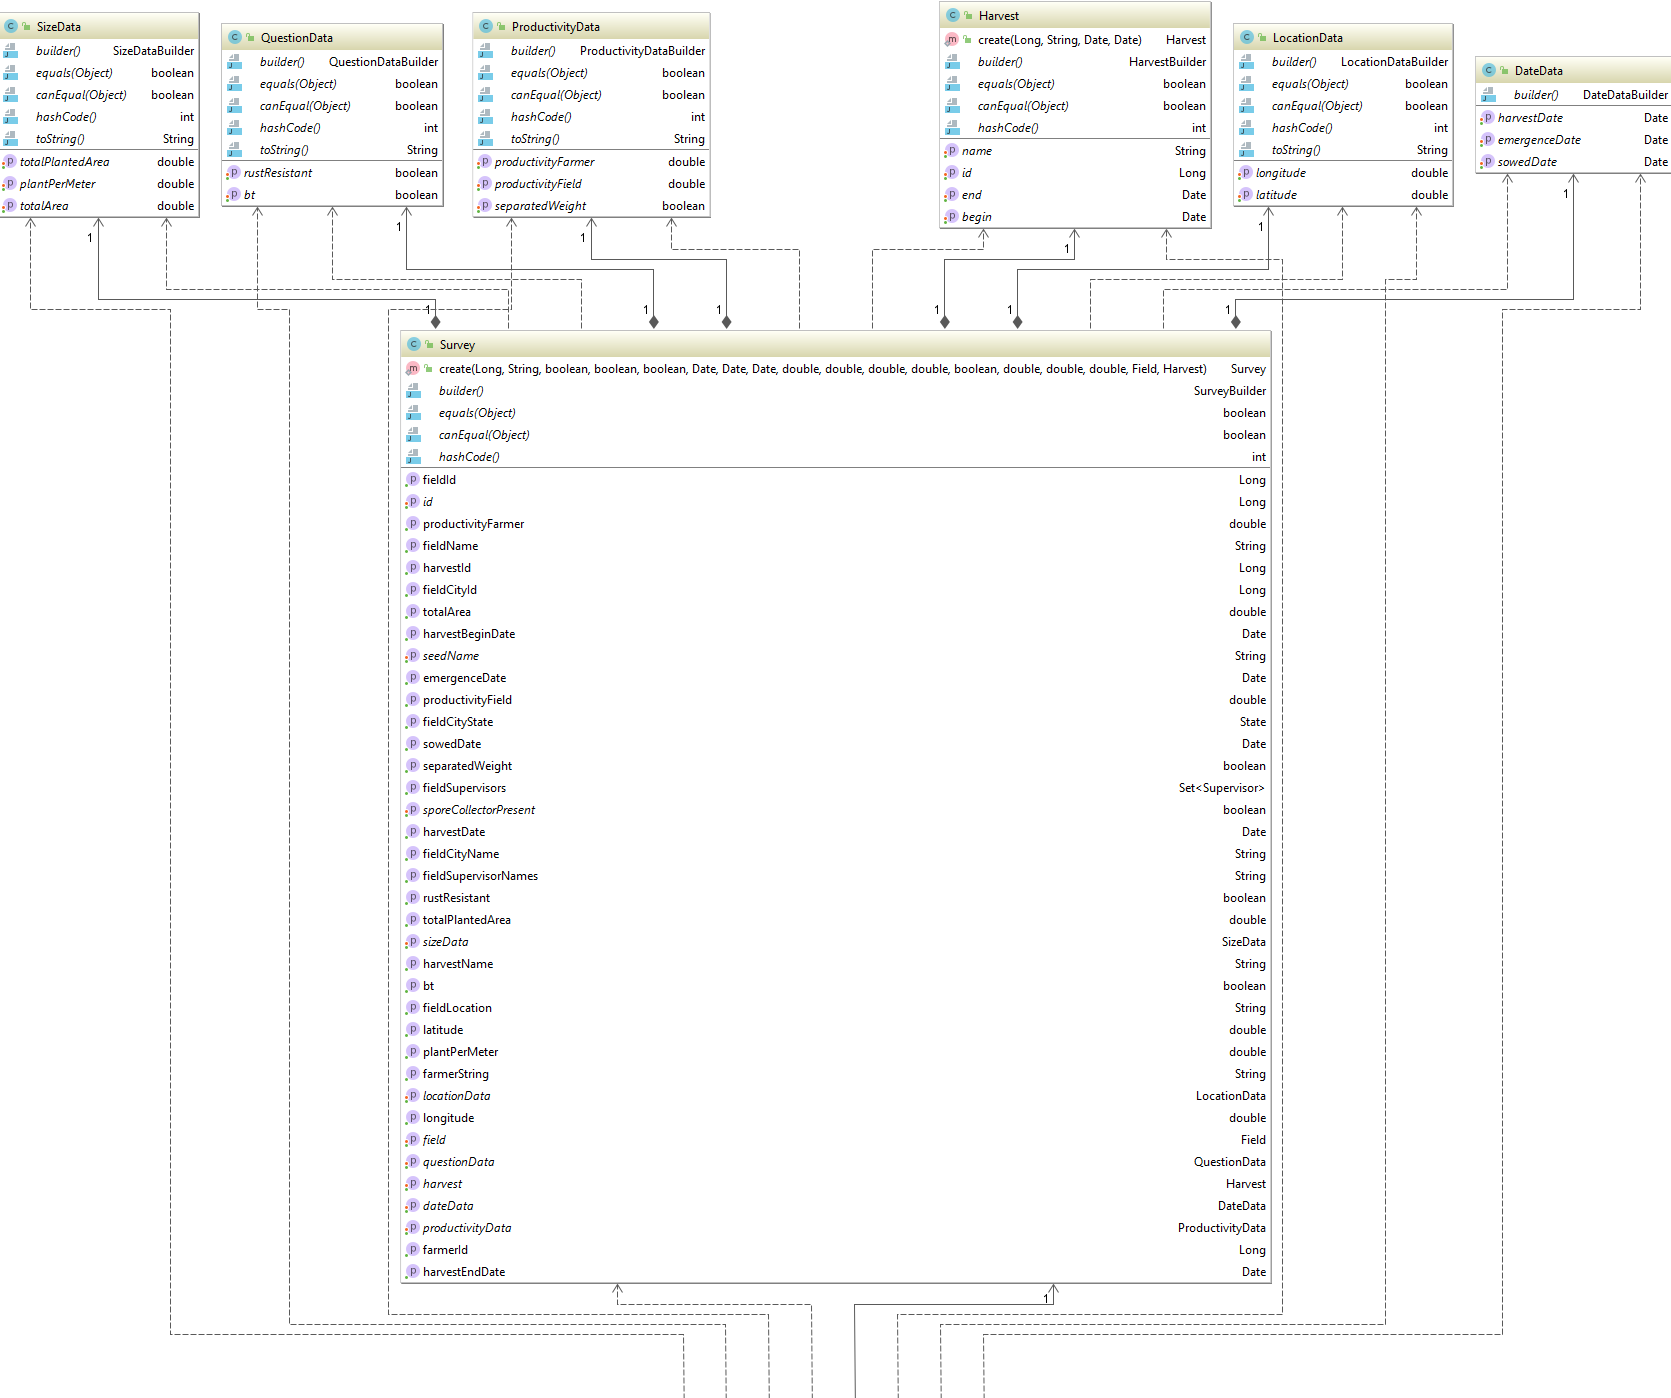
\includegraphics[scale=0.38]{dados/figuras/packSurvei.png}
\end{figure}

\begin{figure}[H]
	\centering
	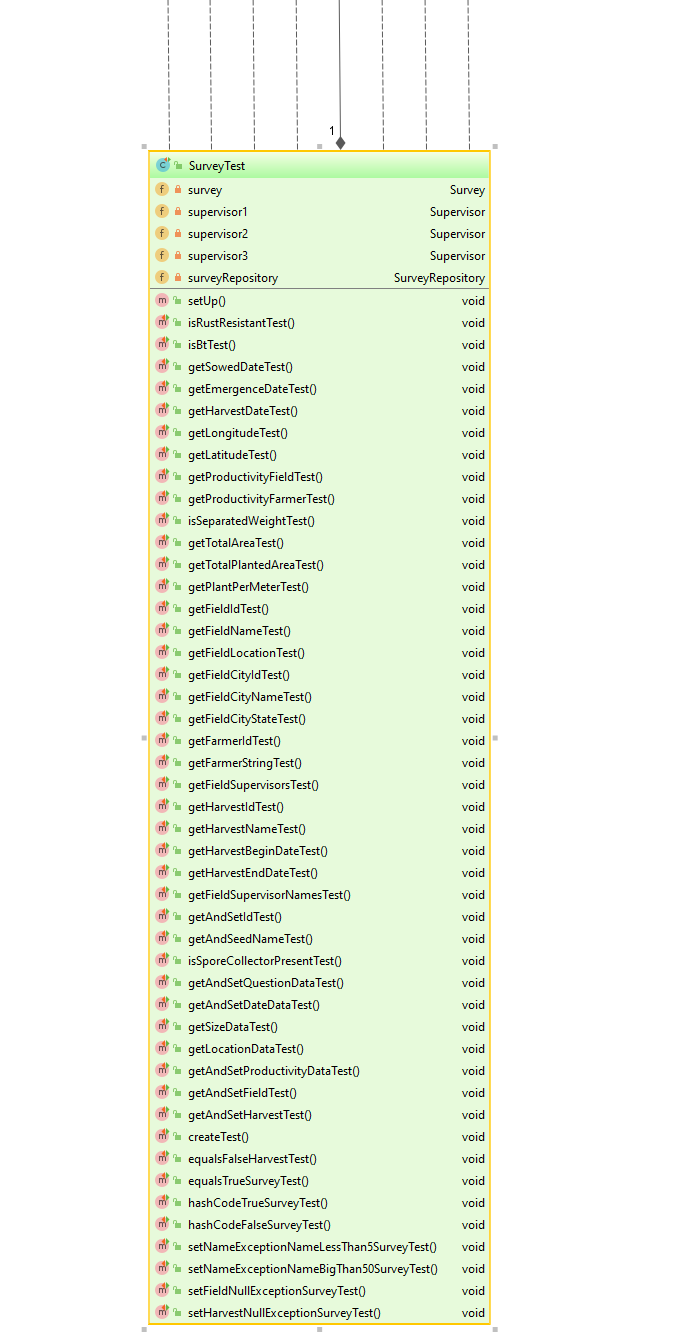
\includegraphics[scale=0.7]{dados/figuras/surveyTest.png}
	\caption{Diagrama de classes Survey e SurveyTest.java.}
	\label{classesSurvey}
\end{figure}

A classe de teste apresentada na FIGURA \ref{classesSurvey} possui 46 métodos de teste é um método de apoio aos testes denominado \textit{“setUp”}, o objetivo dos testes é exercitar a classe \textit{Survey} até que todos as variáveis, entradas e saídas de dados sejam executados pelo menos uma vez. Como a classe \textit{Survey} é composta por outras classes se faz necessário a instanciação de outras classes como \textit{Harvest}, \textit{Farmer}, \textit{City}, \textit{SizeData} e outras para a execução completa dos testes. Como a classe se trata de uma entidade que será persistida em um banco de dados, ela possui certas regras de negócio que serão ativadas somente no momento de gravar os dados no banco, sendo assim foi preciso criar uma referência para a interface \textit{SurveyRepository}, classe responsável por realizar a persistência dos dados no banco. Como o objetivo deste trabalho é cobrir o sistema com testes unitários e testes que integram classes entidades com o banco de dados ou comunicação com \textit{APIs} são testes de integração foi utilizado um \textit{“Mock”} para simular o comportamento do repositório.


A FIGURA \ref{testSurvey} apresenta a declaração da classe de teste, os atributos utilizados para desenvolver os testes e o método \textit{“setUp”} utilizado para preparar o ambiente para os testes.

O trecho de código da FIGURA \ref{testSurvey} apresenta as seguintes funcionalidades:

\begin{itemize}

    \item Na linha 1 é utilizada a anotação \textit{@FixMethodOrder} que permite definir uma ordem de execução dos testes, neste casso foi definida a ordem \textit{“NAME\_ASCENDING"} que faz a execução dos testes de acordo com o nome de maneira ascendente;
    
    \item Linha 2 a classe \textit{SurveyTest} é aberta;

    \item Na linha 4 é feita a declaração do objeto \textit{Survey}, nas linhas 5, 6 e 7  são declarados e instanciados objetos do tipo \textit{Supervisor};

    \item Na linha 8 um objeto do tipo \textit{SurveyRepositorio} é declarado e instanciado como um objeto \textit{mock};

    \item Na linha 10 é utilizado a anotação \textit{@Before}, esta anotação determina que sempre antes da execução de um teste o método \textit{“setUp”} deve ser executado primeiro.

    \item O método \textit{“setUp”} que tem sua declaração na linha 11 e vai até a linha 32, ele é responsável por realizar a construção do objeto \textit{Survey} declarado na linha 4.

\end{itemize}{}


A FIGURA \ref{testSurvey} apresenta os casos de testes criados para a classe \textit{Survey}. 


A ideia geral na elaboração dos testes é a de cobrir cada atribuição de dados, as entrada e saída de dados da classe \textit{Survey}, buscando a cobertura de 100\% das linhas métodos e atributo da classe. Os resultados obtidos da execução dos testes foram listados a seguir:



\begin{figure}[H]
	\centering
	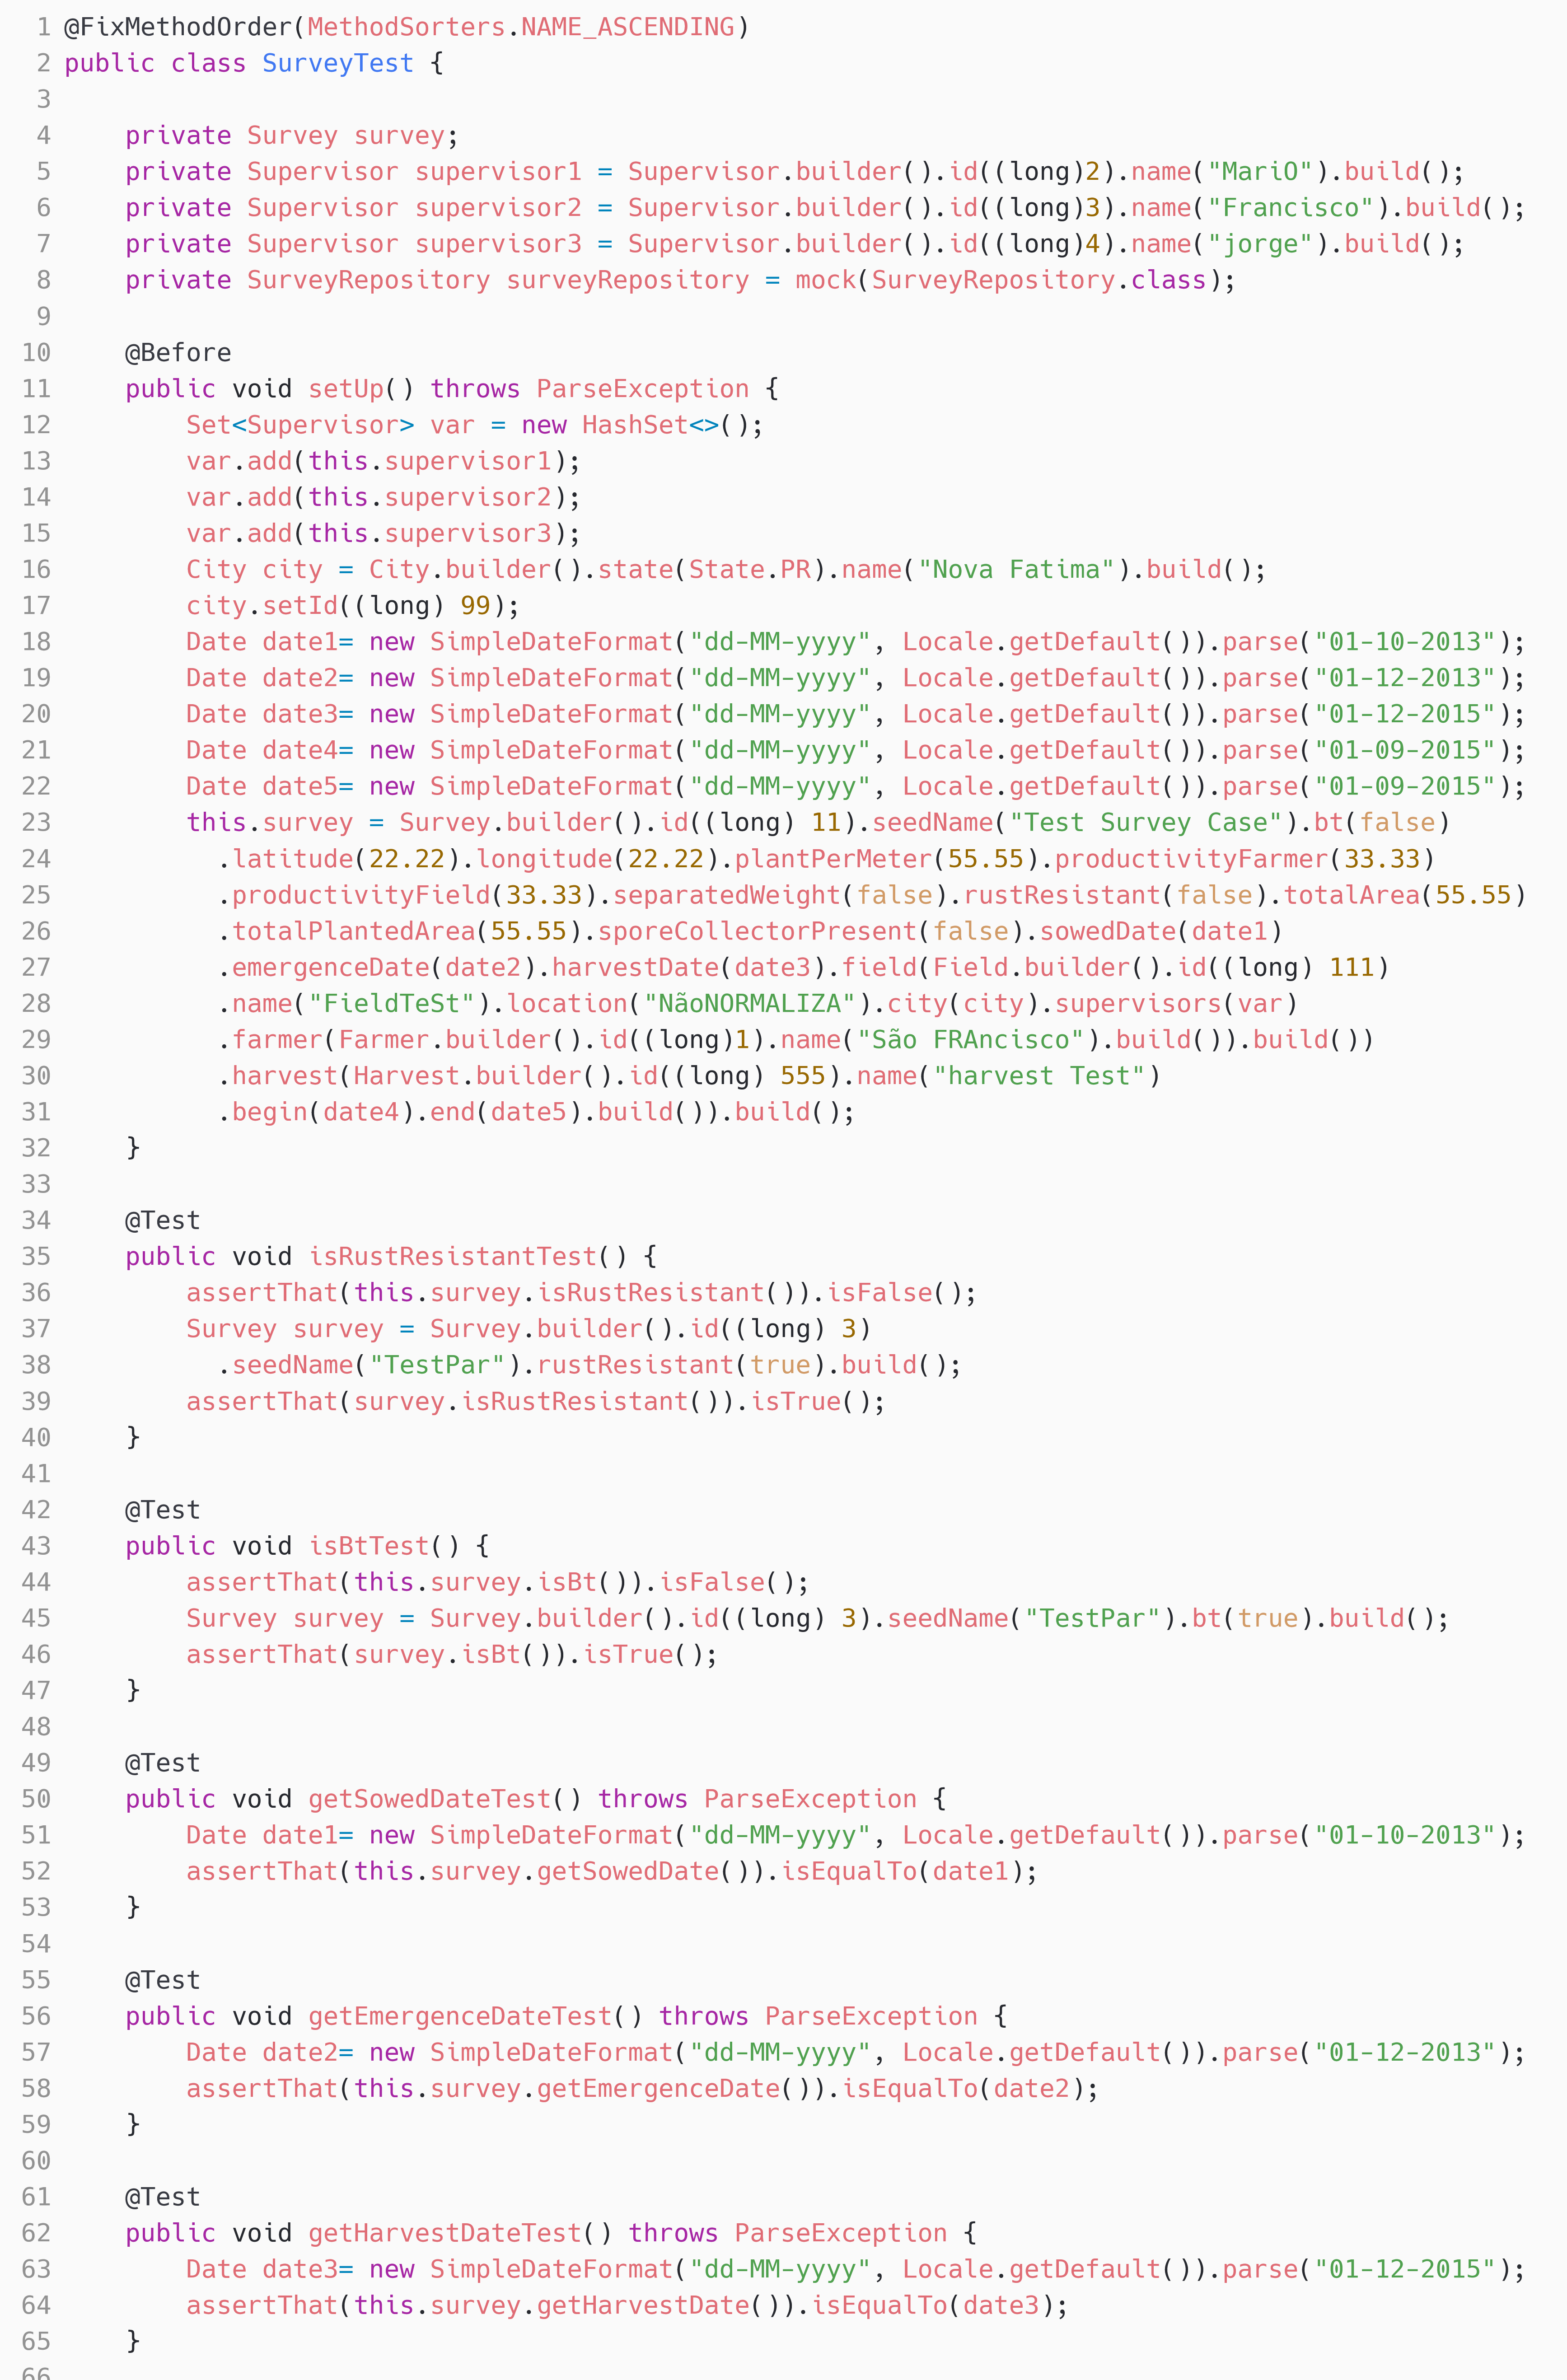
\includegraphics[scale=0.17]{dados/figuras/buildSurvey.png}
\end{figure}

\begin{figure}[H]
	\centering
	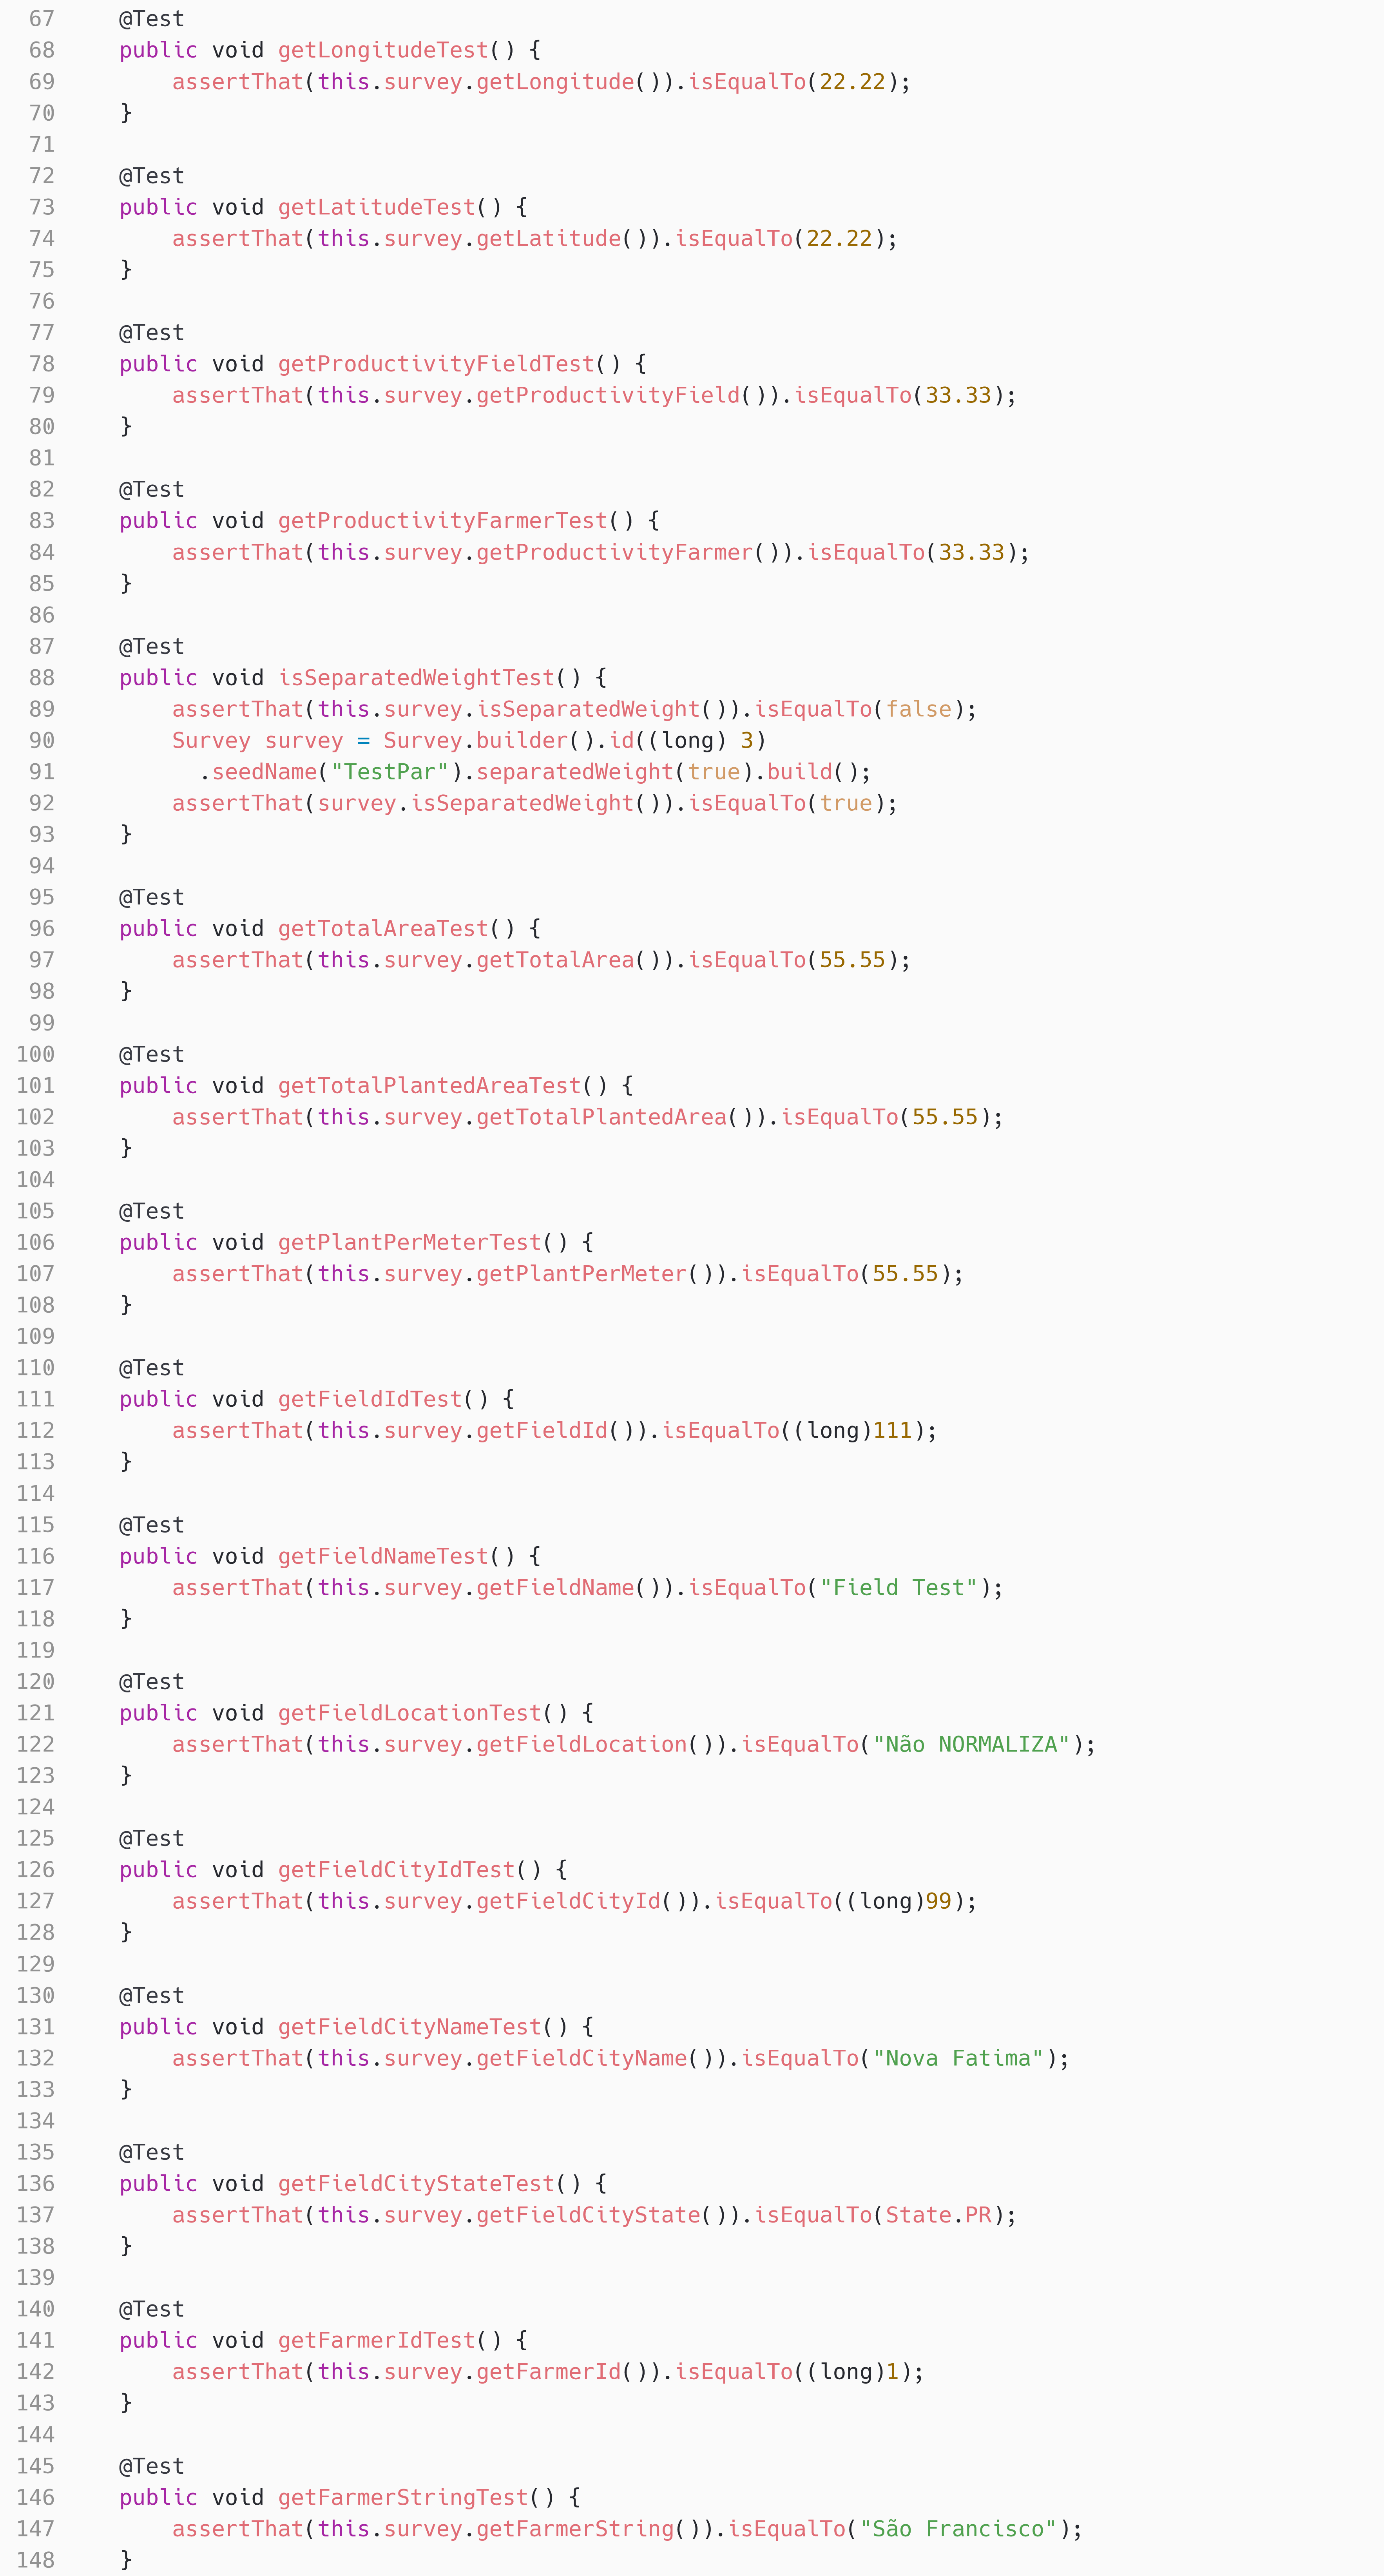
\includegraphics[scale=0.14]{dados/figuras/surveyTest1.png}
\end{figure}

\begin{figure}[H]
	\centering
	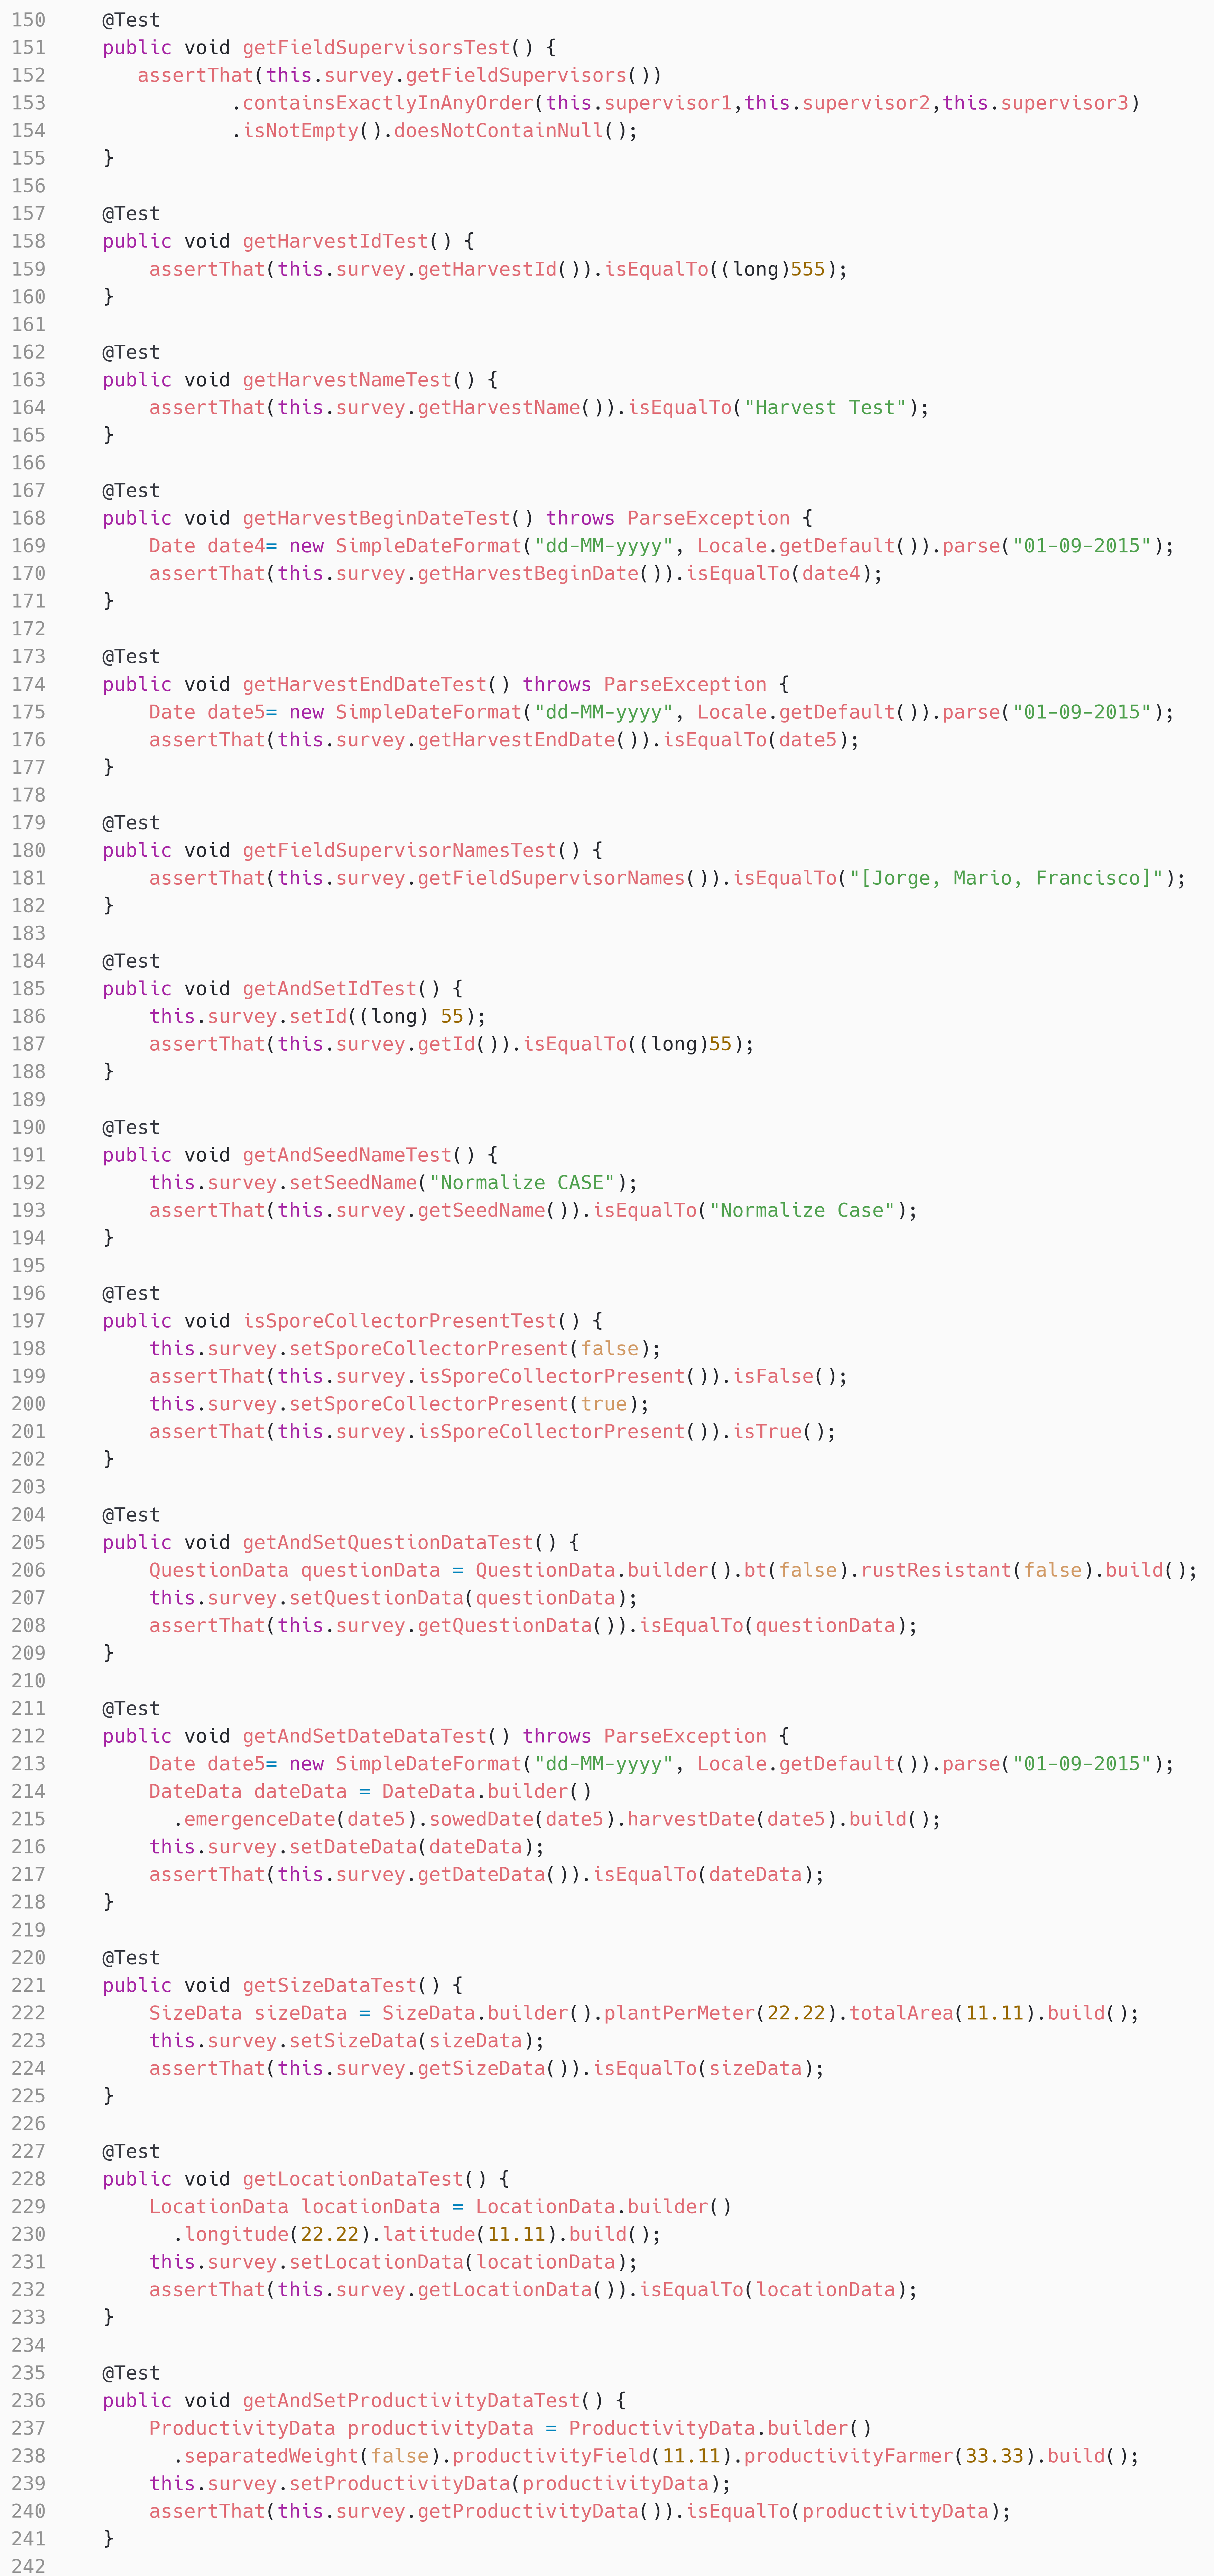
\includegraphics[scale=0.13]{dados/figuras/surveyTest2.png}
\end{figure}

\begin{figure}[H]
	\centering
	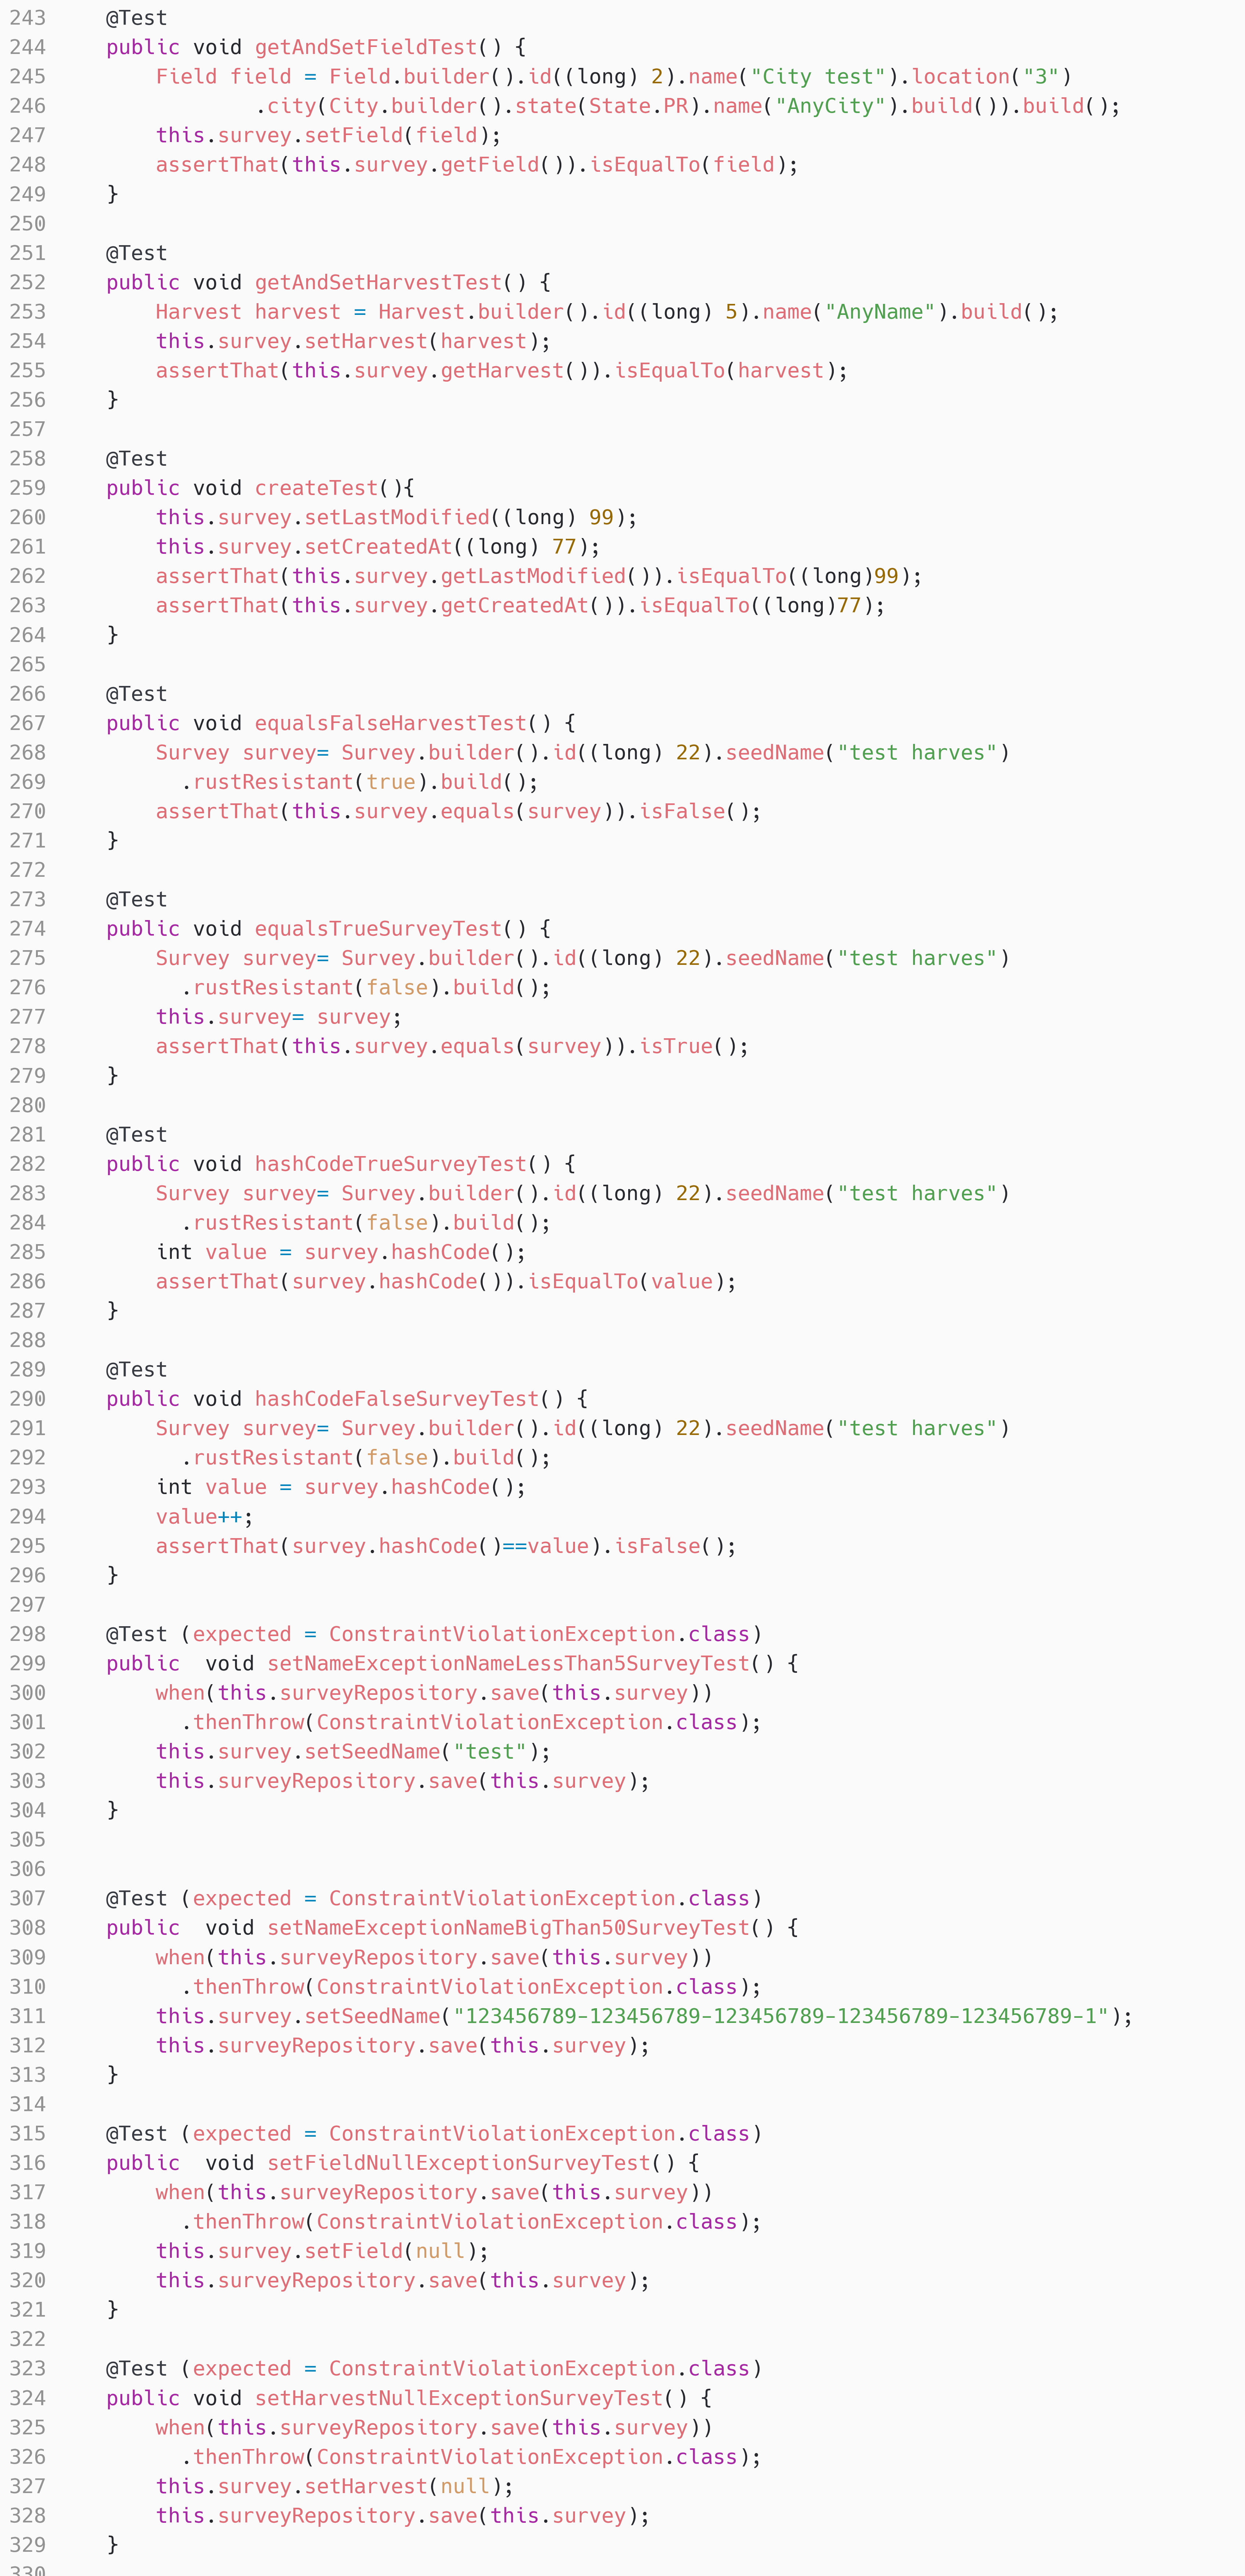
\includegraphics[scale=0.13]{dados/figuras/surveyTest3.png}
	\caption{Classe de Teste SurveyTest.java.}
	\label{testSurvey}
\end{figure}

Método de teste\textit{ “isRustResistantTest()”} linhas 34 a 40 figura \ref{testSurvey}:  Este método de teste consiste em recuperar o valor atribuído a variável\textit{ “rustResistant”} do objeto \textit{“Survey”.} A entrada é um \textit{“boolean”}(verdadeiro ou falso), a saída também se trata de um \textit{“boolean”}. A primeira assertiva recupera o valor atribuído na linha 25, \textit{“FALSE”}, e a saída do meto testado é um\textit{ “FALSE”}, linha 36, em seguida é atribuído a variável o valor \textit{“TRUE”}, linha 37 e 38, uma nova assertiva é feita e o valor recuperado é um \textit{“TRUE”}, linha 39.

Método de teste \textit{“isBtTest ()”} linhas 42 a 47 figura \ref{testSurvey}: Este método de teste consiste em recuperar o valor atribuído a variável\textit{ “bt”} do objeto \textit{“Survey”}. A entrada e um \textit{“boolean”}(verdadeiro ou falso), a saída também se trata de um \textit{“boolean”}. A primeira assertiva recupera o valor atribuído na linha 23, \textit{“FALSE”}, e a saída do meto testado é um \textit{“FALSE”}, linha 44, em seguida é atribuída a variável o valor \textit{“TRUE”}, linha 45 e 46, uma nova assertiva é feita e o valor recuperado é um \textit{“TRUE”}, linha 46.

Método de teste \textit{“getSowedDateTest()”} linhas 49 a 53 figura \ref{testSurvey}: Este teste consiste em recuperar a data atribuída a variável “\textit{“SowedDate”}” do objeto \textit{“Survey”}. A entrada é um objeto do tipo “\textit{“Date”}” que contém o valor de uma data com dia, mês e ano. A saída é um objeto do tipo “\textit{“Date”}” que contem o valor de uma data válida. A entrada é definida na linha 26, um outro objeto do tipo \textit{“Date”} é criado para comparação na linha 51. A assertiva é feita na linha 52 e compara o valor recuperado do meto testado com o valor definido na linha 51, os valores são iguais.  

Método de teste \textit{“getEmergenceDateTest()”} linhas 55 a 59 figura \ref{testSurvey}: Este teste consiste em recuperar a data atribuída a variável \textit{“EmergenceDate”} do objeto \textit{“Survey”}. A entrada é um objeto do tipo \textit{“Date”} que contém o valor de uma data com dia, mês e ano. A saída é um objeto do tipo \textit{“Date”} que contém o valor de uma data válida. A entrada é definida na linha 27, um outro objeto do tipo \textit{“Date”} é criado para comparação na linha 57. A assertiva é feita na linha 58 e compara o valor recuperado do meto testado com o valor definido na linha 57, os valores são iguais.  

Método de teste \textit{“getHarvestDateTest()”} linhas 61 a 65 figura \ref{testSurvey}: Este teste consiste em recuperar a data atribuída a variável \textit{“HarvestDate”} do objeto \textit{“Survey”}. A entrada é um objeto do tipo \textit{“Date”} que contém o valor de uma data com dia, mês e ano. A saída é um objeto do tipo \textit{“Date”} que contém o valor de uma data válida. A entrada é definida na linha 27, um outro objeto do tipo \textit{“Date”} é criado para comparação na linha 63. A assertiva é feita na linha 64 e compara o valor recuperado do meto testado com o valor definido na linha 63, os valores são iguais.  

Método de teste \textit{“getLongitudeTest()”} linhas 67 a 71 figura \ref{testSurvey}: Este teste consiste em recuperar o valor atribuído a variável \textit{“Longitude” }do objeto \textit{“LocationData”}  presente em uma pesquisa. A entrada consiste em um valor numérico de ponto flutuante \textit{“Double”} e a saída também consiste em um valor numérico do tipo \textit{“Double”}. A entrada é realizada na linha 24, o método é testado na linha 69, o retorno é o mesmo valor atribuído na linha 24.   

Método de teste \textit{“getLatitudeTest()”} linhas 72 a 75 figura \ref{testSurvey}: Este teste consiste em recuperar o valor atribuído a variável\textit{ “Latitude”} do objeto \textit{“LocationData”} presente em uma pesquisa. A entrada consiste em um valor numérico de ponto flutuante \textit{“Double”} e a saída também consiste em um valor numérico do tipo \textit{“Double”}. A entrada é realizada na linha 24, o método é testado na linha 74, o retorno é o mesmo valor atribuído na linha 24.

Método de teste \textit{“getProductivityFieldTest()”} linhas 77 a 80 figura \ref{testSurvey}: Este teste consiste em recuperar o valor atribuído a variável “productivityField” do objeto \textit{“ProductivityData”} presente em uma pesquisa. A entrada consiste em um valor numérico de ponto flutuante \textit{“Double”} e a saída também consiste em um valor numérico do tipo \textit{“Double”}. A entrada é realizada na linha 24, o método é testado na linha 74, o retorno é o mesmo valor atribuído na linha 24.

Método de teste \textit{“getProductivityFarmerTest()”} linhas 82 a 85 figura \ref{testSurvey}: Este teste consiste em recuperar o valor atribuído a variável\textit{ “productivityFarmer”} do objeto \textit{“ProductivityData”} presente em uma pesquisa. A entrada consiste em um valor numérico de ponto flutuante \textit{“Double”} e a saída também consiste em um valor numérico do tipo \textit{“Double”}. A entrada é realizada na linha 24, o método é testado na linha 79, o retorno é o mesmo valor atribuído na linha 24.

Método de teste \textit{“isSeparatedWeightTest()”} linhas 87 a 93 figura \ref{testSurvey}: Este método de teste consiste em recuperar o valor atribuído a variável\textit{ “SeparatedWeight”} do objeto \textit{“ProductivityData”} presente em uma pesquisa. A entrada e um \textit{“boolean”}(verdadeiro ou falso), a saída também se trata de um \textit{“boolean”}. A primeira assertiva recupera o valor atribuído na linha 25, \textit{“FALSE”}, e a saída do meto testado é um \textit{“FALSE”}, linha 44, em seguida é atribuída a variável o valor \textit{“TRUE”}, linha 90 e 91, uma nova assertiva é feita é o valor recuperado é um \textit{“TRUE”}, linha 92.

Método de teste \textit{“getTotalAreaTest()”} linhas 95 a 98 figura \ref{testSurvey}: Este teste consiste em recuperar o valor atribuído a variável\textit{ “TotalArea”} do objeto \textit{“SizeData”} presente em uma pesquisa. A entrada consiste em um valor numérico de ponto flutuante \textit{“Double”} e a saída também consiste em um valor numérico do tipo \textit{“Double”}. A entrada é realizada na linha 25, o método é testado na linha 97, o retorno é o mesmo valor atribuído na linha 25.

Método de teste \textit{“getTotalPlantedAreaTest()”} linhas 100 a 103 figura \ref{testSurvey}: Este teste consiste em recuperar o valor atribuído a variável \textit{“TotalPlantedArea”} do objeto \textit{“SizeData”} presente em uma pesquisa. A entrada consiste em um valor numérico de ponto flutuante \textit{“Double”} e a saída também consiste em um valor numérico do tipo \textit{“Double”}. A entrada é realizada na linha 26, o método é testado na linha 102, o retorno é o mesmo valor atribuído na linha 26.

Método de teste \textit{“getPlantPerMeterTest()”} linhas 105 a 108 figura \ref{testSurvey}: Este teste consiste em recuperar o valor atribuído a variável\textit{ “plantPerMeter”} do objeto \textit{“SizeData”} presente em uma pesquisa. A entrada consiste em um valor numérico de ponto flutuante \textit{“Double”} e a saída também consiste em um valor numérico do tipo \textit{“Double”}. A entrada é realizada na linha 24, o método é testado na linha 107, o retorno é o mesmo valor atribuído na linha 24.

Método de teste \textit{“getFieldIdTest()”} linhas 110 a 113 figura \ref{testSurvey}: Este teste consiste em recuperar o identificador único de um objeto \textit{“Field”} presente em uma pesquisa. A entrada consiste em um objeto do tipo \textit{“Field”} que possui um identificador único, a saída é o identificador único, um valor numérico do tipo \textit{“Long”}. A entrada é feita nas linhas 27 e 28, a assertiva é feia na linha 112, o valor recuperado é o mesmo atribuído na linha 27.

Método de teste\textit{ “getFieldNameTest()”} linhas 115 a 118 figura \ref{testSurvey}: Este teste consiste em recuperar o nome atribuído a um objeto \textit{“Field”} presente em uma pesquisa. A entrada consiste em um objeto do tipo \textit{“Field”} que possui um nome, a saída é o nome contido no objeto, uma \textit{String”} de caracteres normalizados com o primeiro caractere de cada conjunto de caracteres maiúsculo. A entrada é feita nas linhas 27 e 28, a assertiva é feia na linha 117, o valor recuperado é o mesmo atribuído na linha 27 mais com o primeiro caractere de cada conjunto maiúsculo.

Método de teste \textit{“getFieldLocationTest()”} linhas 120 a 123 figura \ref{testSurvey}: Este teste consiste em recuperar a localização atribuída a um objeto \textit{“Field”} presente em uma pesquisa. A entrada consiste em um objeto do tipo \textit{“Field”} que possui uma localização, a saída é a localização contida no objeto, uma \textit{“String”} de caracteres. A entrada é feita nas linhas 27 e 28, a assertiva é feia na linha 122, o valor recuperado é o mesmo atribuído na linha 27.

Método de teste\textit{ “getFieldCityIdTest()”} linhas 125 a 128 figura \ref{testSurvey}: Este teste consiste em recuperar o identificador único de um objeto \textit{“City”} presente em uma pesquisa. A entrada consiste em um objeto do tipo \textit{“Field”} que possui uma cidade com identificador único, a saída é o identificador do único da cidade, um valor numérico do tipo \textit{“Long”}. O objeto \textit{“City”} é criado nas linhas 16 e 17, a entrada é feita nas linhas 27 e 28, a assertiva é feia na linha 127, o valor recuperado é o mesmo atribuído na linha 17.


Método de teste \textit{“getFieldCityNameTest()”} linhas 130 a 133 figura \ref{testSurvey}: Este teste consiste em recuperar o nome de um objeto \textit{“City”} presente em uma pesquisa. A entrada consiste em um objeto do tipo \textit{“Field”} que possui uma cidade com um nome, a saída é uma \textit{“String”} de caracteres normalizados com o primeiro caractere de cada conjunto maiúsculo. O objeto \textit{“City”} é criado nas linhas 16, a entrada é feita nas linhas 27 e 28, a assertiva é feia na linha 132, o valor recuperado é o mesmo atribuído na linha 16 mais com o primeiro caractere de cada conjunto maiúsculo.

Método de teste \textit{“getFieldCityStateTest()”} linhas 135 a 138 figura \ref{testSurvey}: Este teste consiste em recuperar o estado de um objeto \textit{“City”} presente em uma pesquisa. A entrada consiste em um objeto do tipo \textit{“Field”} que possui uma cidade com um estado, a saída é um objeto do tipo \textit{“State.PR”}. O objeto \textit{“City”} é criado nas linhas 16, a entrada é feita nas linhas 27 e 28, a assertiva é feia na linha 137, o valor recuperado é o mesmo atribuído na linha 16.

Método de teste \textit{“getFarmerIdTest()”} linhas 140 a 143 figura \ref{testSurvey}: Este teste consiste em recuperar o identificador único de um objeto \textit{“Farmer”} presente em uma pesquisa. A entrada consiste em um objeto do tipo \textit{“Field”} que possui um agricultor com identificador único, a saída é o identificador do único do agricultor, um valor numérico do tipo \textit{“Long”}. O objeto \textit{“Farmer”} é criado na linha 29, a entrada é feita na linha 27, 28 e 29, a assertiva é feia na linha 142, o valor recuperado é o mesmo atribuído na linha 29.

Método de teste \textit{“getFarmerStringTest()”} linhas 145 a 148 figura \ref{testSurvey}: Este teste consiste em recuperar o nome de um objeto \textit{“Farmer”} presente em uma pesquisa. A entrada consiste em um objeto do tipo \textit{“Field”} que possui um agricultor com um nome, a saída é uma \textit{“String”} de caracteres normalizados com o primeiro caractere de cada conjunto maiúsculo. O objeto \textit{“Farmer”} é criado nas linhas 29, a entrada é feita nas linhas 27, 28 e 29, a assertiva é feia na linha 147, o valor recuperado é o mesmo atribuído na linha 29 mais com o primeiro caractere de cada conjunto maiúsculo.

Método de teste \textit{“getFieldSupervisorsTest()”} linhas 150 a 155 figura \ref{testSurvey}: Este teste consiste em recuperar os supervisores presentes em um objeto \textit{“Field”} presente em uma pesquisa. A entrada consiste em um objeto do tipo \textit{“Field”} que possua um ou mais supervisores, a saída é uma lista de objetos do tipo \textit{“Supervisor”} que contem os supervisores presentes no \textit{“Field”} presente na pesquisa. Uma lista de supervisores é criada nas linhas 12 a 15, a entrada é feita nas linhas 27, 28 e 29, a assertiva é feia nas linhas 152 e 153, o valor recuperado e uma lista de supervisores que contem os supervisores declarados nas linhas 5, 6 e 7.


Método de teste \textit{“getHarvestIdTest()”} linhas 157 a 160 figura \ref{testSurvey}: Este teste consiste em recuperar o identificador único de um objeto \textit{“Harvest”} presente em uma pesquisa. A entrada consiste em um objeto do tipo \textit{“Harvest”} que possui um identificador único, a saída é o identificador do único da colheita, um valor numérico do tipo \textit{“Long”}. O objeto \textit{“Harvest”} é criado na linha 30, a entrada é feita nas linhas 27, 28, 29 e 30 a assertiva é feia na linha 159, o valor recuperado é o mesmo atribuído na linha 30.

Método de teste \textit{“getHarvestNameTest()”} linhas 162 a 165 figura \ref{testSurvey}: Este teste consiste em recuperar o nome de um objeto \textit{“Harvest”} presente em uma pesquisa. A entrada consiste em um objeto do tipo \textit{“Harvest”} que possui um nome, a saída é uma \textit{“String”} de caracteres normalizados com o primeiro caractere de cada conjunto maiúsculo. O objeto \textit{“Harvest”} é criado nas linhas 30, a entrada é feita nas linhas 27, 28, 29 e 30, a assertiva é feia na linha 164, o valor recuperado é o mesmo atribuído na linha 30 mais com o primeiro caractere de cada conjunto maiúsculo.

Método de teste \textit{“getHarvestBeginDateTest()”} linhas 167 a 171 figura \ref{testSurvey}: Este teste consiste em recuperar a data da variável \textit{“BeginDate”} atribuída a um objeto \textit{“Harvest”} presente em uma pesquisa. A entrada é um objeto do tipo \textit{“Harvest”} que possui um \textit{“Date”} que contém o valor de uma data com dia, mês e ano. A saída é um objeto do tipo \textit{“Date”} que contém o valor de uma data válida. A entrada é definida na linha 30, um outro objeto do tipo \textit{“Date”} é criado para comparação na linha 169. A assertiva é feita na linha 170 e compara o valor recuperado do meto testado com o valor definido na linha 169, os valores são iguais.  

Método de teste \textit{“getHarvestEndDateTest()”} linhas 173 a 177 figura \ref{testSurvey}: Este teste consiste em recuperar a data da variável \textit{“EndDate” }atribuída a um objeto \textit{“Harvest”} presente em uma pesquisa. A entrada é um objeto do tipo \textit{“Harvest”} que possui um \textit{“Date”} que contém o valor de uma data com dia, mês e ano. A saída é um objeto do tipo \textit{“Date”} que contém o valor de uma data válida. A entrada é definida na linha 30, um outro objeto do tipo \textit{“Date”} é criado para comparação na linha 175. A assertiva é feita na linha 176 e compara o valor recuperado do meto testado com o valor definido na linha 175, os valores são iguais.  

Método de teste \textit{“getFieldSupervisorNamesTest()”} linhas 179 a 182 figura \ref{testSurvey}: Este teste consiste em recuperar os nomes dos supervisores presentes em um objeto \textit{“Field”} presente em uma pesquisa. A entrada consiste em um objeto do tipo \textit{“Field”} que possua um ou mais supervisores, a saída é uma \textit{“String”} que contém os nomes dos supervisores presentes no objeto \textit{“Field”} presente na pesquisa. Uma lista de supervisores é criada nas linhas 12 a 15, a entrada é feita nas linhas 27, 28 e 29, a assertiva é feia nas linhas 181, o valor recuperado e uma \textit{“String”} com o nome dos supervisores declarados nas linhas 5, 6 e 7.

Método de teste \textit{“getAndSetIdTest()”} linhas 184 a 188 figura \ref{testSurvey}: Este teste consiste em atribuir e recuperar o identificador único de uma pesquisa. A entrada consiste em um valor numérico do tipo \textit{“Long”}, a saída é um valor numérico do tipo \textit{“Long”}. A entrada e feita na linha 186, a saída e feita na assertiva linha 187, que compara a saída com o valor atribuído, os valores são iguais.

Método de teste \textit{“getAndSeedNameTest()”} linhas 190 a 194 figura \ref{testSurvey}: Este teste trata de atribuir um valor da variável \textit{“Seed”} do tipo \textit{“String”} do objeto \textit{“Survey”}. A entrada consiste em uma \textit{“String”} de caracteres, a saída é uma string de caracteres normalizada. A assertiva é feita na linha 193 e o valor recuperado é idêntico ao atribuído, mas com a primeira letra de cada conjunto de caracteres maiúscula.

Método de teste \textit{“isSporeCollectorPresentTest()”} linhas 196 a 202 figura \ref{testSurvey}: Este método de teste consiste em recuperar o valor atribuído a variável \textit{“SporeCollectorPresent” }do objeto \textit{“Survey”}. A entrada e um \textit{“boolean”}(verdadeiro ou falso), a saída também se trata de um \textit{“boolean”}. A primeira assertiva recupera o valor atribuído na linha 198, \textit{“FALSE”}, e a saída do meto testado é um \textit{“FALSE”}, linha 199, em seguida é atribuída a variável o valor \textit{“TRUE”}, linha 200, uma nova assertiva é feita é o valor recuperado é um \textit{“TRUE”}, linha 201.

Método de teste \textit{“getAndSetQuestionDataTest()”} linhas 204 a 209 figura \ref{testSurvey}: Este teste trata de atribuir um objeto do tipo \textit{“QuestionData” }a \textit{“Survey”} em seguida faz a recuperação do mesmo. A entrada é um objeto do tipo \textit{“QuestionData”,} a saída é um objeto do tipo\textit{ “QuestionData”}. A entrada é feita na linha 207, a saída é feita a linha 208 juntamente da assertiva que compara o objeto recuperado com o objeto inserido, os dois são iguais.

Método de teste \textit{“getAndSetDateDataTest()”} linhas 211 a 218 figura \ref{testSurvey}: Este teste trata de atribuir um objeto do tipo \textit{“DateData”} a \textit{“Survey”} em seguida faz a recuperação do mesmo. A entrada é um objeto do tipo “DateData”, a saída é um objeto do tipo \textit{“DateData”}. A entrada é feita na linha 216, a saída é feita a linha 217 juntamente da assertiva que compara o objeto recuperado com o objeto inserido, os dois são iguais.

Método de teste \textit{“getSizeDataTest()”} linhas 220 a 225 figura \ref{testSurvey}: Este teste trata de atribuir um objeto do tipo \textit{“SizeData”} a \textit{“Survey”} em seguida faz a recuperação do mesmo. A entrada é um objeto do tipo “SizeData”, a saída é um objeto do tipo \textit{“SizeData”}. A entrada é feita na linha 223, a saída é feita a linha 224 juntamente da assertiva que compara o objeto recuperado com o objeto inserido, os dois são iguais.

Método de teste \textit{“getLocationDataTest()”} linhas 227 a 233 figura \ref{testSurvey}: Este teste trata de atribuir um objeto do tipo \textit{“LocationData”} a \textit{“Survey”} em seguida faz a recuperação do mesmo. A entrada é um objeto do tipo \textit{“LocationData”}, a saída é um objeto do tipo \textit{“LocationData”}. A entrada é feita na linha 231, a saída é feita a linha 232 juntamente da assertiva que compara o objeto recuperado com o objeto inserido, os dois são iguais.

Método de teste \textit{“getAndSetProductivityDataTest()”} linhas 235 a 241 figura \ref{testSurvey}: Este teste trata de atribuir um objeto do tipo \textit{“ProductivityData” }a \textit{“Survey”} em seguida faz a recuperação do mesmo. A entrada é um objeto do tipo \textit{“ProductivityData”}, a saída é um objeto do tipo “ProductivityData”. A entrada é feita na linha 239, a saída é feita a linha 240 juntamente da assertiva que compara o objeto recuperado com o objeto inserido, os dois são iguais.

Método de teste \textit{“getAndSetFieldTest()”} linhas 243 a 249 figura \ref{testSurvey}: Este teste trata de atribuir um objeto do tipo \textit{“Field”} a \textit{“Survey”} em seguida faz a recuperação do mesmo. A entrada é um objeto do tipo \textit{“Field”}, a saída é um objeto do tipo \textit{“Field”}. A entrada é feita na linha 247, a saída é feita a linha 248 juntamente da assertiva que compara o objeto recuperado com o objeto inserido, os dois são iguais.

Método de teste \textit{“getAndSetHarvestTest()”} linhas 251 a 256 figura \ref{testSurvey}: Este teste trata de atribuir um objeto do tipo \textit{“Harvest”} a \textit{“Survey”} em seguida faz a recuperação do mesmo. A entrada é um objeto do tipo \textit{“Harvest”}, a saída é um objeto do tipo \textit{“Harvest”}. A entrada é feita na linha 254, a saída é feita a linha 255 juntamente da assertiva que compara o objeto recuperado com o objeto inserido, os dois são iguais.

Método de teste \textit{“createTest()”} linhas 258 a 264 figura \ref{testSurvey}: Este método é responsável por testar os atributos criados na superclasse \textit{“auditingPersistenceEntity”,} como uma superclasse não pode ser testada os métodos e atributos dela devem ser testados em uma das suas subclasses.  A classe e composta por dois atributos do tipo long \textit{“LastModified” }e \textit{“CreatedAt”}, O objetivo deste teste é de atribuir valor as variáveis e verificar se os valores atribuídos são recuperados corretamente. As entradas foram criadas nas linhas 260 e 261 respectivamente. Posteriormente nas linhas 262 e 263 e feita a confirmação das saídas contendo os valores 99 e 77 do tipo \textit{“Long”}.

Método de teste \textit{“equalsFalseHarvestTest()”} linhas 266 a 272 figura \ref{testSurvey}: Este método de teste consiste em comparar dois objetos do tipo \textit{“Survey”} caso eles sejam iguais o retorno é um \textit{“boolean”} \textit{“TRUE”} caso sejam diferentes o retorno é um \textit{“FALSE”}. A entrada consiste em dois objetos do tipo \textit{“Survey”}, o primeiro objeto é criado nas linhas 26, 27, 28 e 29, o segundo objeto é criado nas linhas 268 e 269. A saída é um \textit{“FALSE”} pois os objetos comparados são diferentes.

Método de teste \textit{“equalsTrueSurveyTest()”} linhas 273 a 279 figura \ref{testSurvey}: Este método de teste consiste em comparar dois objetos do tipo \textit{“Survey”} caso eles sejam iguais o retorno é um \textit{“boolean”} \textit{“TRUE”} caso sejam diferentes o retorno é um \textit{“FALSE”}. A entrada consiste em dois objetos do tipo \textit{“Survey”}, o primeiro objeto é criado nas linhas 26, 27, 28 e 29, o segundo objeto é criado nas linhas 275 e 276, o primeiro objeto recebe uma cópia do segundo objeto. A saída é um \textit{“TRUE”} pois os objetos são iguais.

Método de teste \textit{“hashCodeTrueSurveyTest()”} linhas 281 a 287 figura \ref{testSurvey}: Este teste consiste em recuperar o valor de \textit{“hashcode”} de um objeto e verifica seu valor em uma segunda chamada. O método não possui entrada. A saída consiste em um valor numérico do tipo \textit{“int”.} O valor de hash é recuperado em uma primeira chamada na linha 285, em seguida é feita uma assertiva, esta compara o valor recuperado anteriormente com o valor de uma nova chamda do método de hash, os valores são iguais.

Método de teste\textit{ “hashCodeFalseSurveyTest()”} linhas 289 a 296 figura \ref{testSurvey}: Este teste consiste em recuperar o valor de \textit{“hashcode”} de um objeto e verifica seu valor em uma segunda chamada. O método não possui entrada. A saída consiste em um valor numérico do tipo\textit{ “int”}. O valor é de hash é recuperado em uma primeira chamada na linha 293, em seguida é feito um incremento no valor recuperado. Uma assertiva compara o valor chamado incrementado com o valor de uma nova chamda do método de hash, os valores são diferentes.


Método de teste \textit{“setNameExceptionNameLessThan5SurveyTest()”} linhas 298 a 304 figura \ref{testSurvey}: Uma das restrições que se encontra na hora de salvar um objeto do tipo \textit{“Survey”} é que a variável “Seed” do tipo \textit{“String”} deve ter entre 5 e 50 caracteres. A entrada consiste em uma \textit{“String”} contendo apenas quatro caractere. A saída esperada é uma exceção de violação das regras do banco. A saída deste teste é uma \textit{“ConstraintViolationException.class”} disparada pelo \textit{“SurveyRepository.class”} pois o valor atribuído é menor que a regra estipulado.

Método de teste “setNameExceptionNameBigThan50SurveyTest()” linhas 307 a 313 figura \ref{testSurvey}: Uma das restrições que se encontra na hora de salvar um objeto do tipo \textit{“Survey”} é que a variável “Seed” do tipo \textit{“String”} deve ter entre 5 e 50 caracteres. A entrada consiste em uma \textit{“String”} contendo apenas cinquenta e um caractere. A saída esperada é uma exceção de violação das regras do banco. A saída deste teste é uma \textit{“ConstraintViolationException.class”} disparada pelo \textit{“SurveyRepository.class” }pois o valor atribuído é maior que a regra estipulado.

Método de teste \textit{“setFieldNullExceptionSurveyTest()”} linhas 315 a 321 figura \ref{testSurvey}: Uma das restrições que se encontra na hora de salvar um objeto do tipo \textit{“Survey”} é que a pesquisa deve possuir um objeto do tipo \textit{“Field”}. A entrada consiste em uma \textit{“null”.} A saída esperada é uma exceção de violação das regras do banco. A saída deste teste é uma \textit{“ConstraintViolationException.class”} disparada pelo \textit{“SurveyRepository.class”} pois o objeto atribuído é nulo.

Método de teste \textit{“setHarvestNullExceptionSurveyTest()”} linhas 323 a 329 figura \ref{testSurvey}: Uma das restrições que se encontra na hora de salvar um objeto do tipo \textit{“Survey”} é que a pesquisa deve possuir um objeto do tipo \textit{“Field”}. A entrada consiste em uma \textit{“null”}. A saída esperada é uma exceção de violação das regras do banco. A saída deste teste é uma\textit{ “ConstraintViolationException.class” }disparada pelo \textit{“SurveyRepository.class” }pois o objeto atribuído é nulo.



Após a execução dos testes a cobertura das entradas e saídas de dados da classe \textit{Survey.java} é de 100\%. 


\section{RESULTADO GERAL DOS TESTES PACOTE ENTITY}

Para alcançar a cobertura de 100\%  de todos os métodos linhas e classes do pacote\textit{Entity}foram criados no total 358 testes de unidade, onde 357 foram aprovados e 1 rejeitado. Cada classe possui o seguinte número de casos de teste: 

\begin{itemize}
        \item Pacote Base:
\begin{itemize}
    \item Classe \textit{FieldTest}: 20 casos de teste aprovados, 1 reprovado;
    \item Classe \textit{RegionTest}: 18 casos de teste aprovados;
    \item Classe \textit{FarmerTest}: 5 casos de teste aprovados;
    \item Classe \textit{StateTest}: 1 casos de teste aprovados;
    \item Classe \textit{MacroRegionTest}: 8 casos de teste aprovados;
    \item Classe \textit{CityTest}: 5 casos de teste aprovados;
    \item Classe \textit{SupervisorTest}: 13 casos de teste aprovados;
\end{itemize}
  \item Pacote MIP:
  \begin{itemize} 
    \item Classe \textit{GrowthPhaseTest}: 1 casos de teste aprovados;
    \item Classe \textit{PestDiseaseTest}: 9 casos de teste aprovados;
    \item Classe \textit{PestNaturalPredatorTest}: 9 casos de teste aprovados;
    \item Classe \textit{PestSizeTest}: 1 casos de teste aprovados;
    \item Classe \textit{PestTest}: 12 casos de teste aprovados;
    \item Classe \textit{MIPSampleNaturalPredatorOccurrenceTest}: 8 casos de teste aprovados;
    \item Classe \textit{MIPSamplePestDiseaseOccurrenceTest}: 8 casos de teste aprovados;
    \item Classe \textit{MIPSamplePestOccurrenceTest}: 10 casos de teste aprovados;
    \item Classe \textit{MIPSampleTest}: 23 casos de teste aprovados;
\end{itemize}
  \item Pacote \textit{Survey}:
  \begin{itemize}   
    \item Classe \textit{SurveyTest}: 8 casos de teste aprovados;46
    \item Classe \textit{HarvestTest}: 11 casos de teste aprovados;
    \item Classe \textit{DateDataTest}: 3 casos de teste aprovados;
    \item Classe \textit{LocationDataTest}: 7 casos de teste aprovados;
    \item Classe \textit{ProductivityDataTest}: 8 casos de teste aprovados;
    \item Classe \textit{QuestionDataTest}: 7 casos de teste aprovados;
    \item Classe \textit{SizeDataTest}: 4 casos de teste aprovados;
\end{itemize}
  \item Pacote MID:
  \begin{itemize}
    \item Classe \textit{BladeReadingResponsibleEntityTest}: 7 casos de teste aprovados;
    \item Classe \textit{AsiaticRustTypesLeafInspectionTest}: 1 casos de teste aprovados;
    \item Classe \textit{AsiaticRustTypesSporeCollectorTest}: 1 casos de teste aprovados;
    \item Classe \textit{MIDSampleFungicideApplicationOccurrenceTest}: 9 casos de teste aprovados;
    \item Classe \textit{MIDSampleLeafInspectionOccurrenceTest}: 7 casos de teste aprovados;
    \item Classe \textit{MIDSampleSporeCollectorOccurrenceTest}: 9 casos de teste aprovados;
    \item Classe \textit{MIDRustSampleTest}: 12 casos de teste aprovados;
    \item Classe \textit{BladeReadingResponsiblePersonTest}: 8 casos de teste aprovados;
    \end{itemize}
    \item Pacote \textit{Pulverisation}:
  \begin{itemize}
    \item Classe \textit{ProductTest}: 16 casos de teste aprovados;
    \item Classe \textit{ProductUnitTest}: 1 casos de teste aprovados;
    \item Classe \textit{PulverisationOperationOccurrenceTest}: 13 casos de teste aprovados;
    \item Classe \textit{PulverisationOperationTest}: 23 casos de teste aprovados;
    \item Classe \textit{TargetCategoryTest}: 1 casos de teste aprovados;
    \item Classe \textit{TargetTest}: 11 casos de teste aprovados;
    \end{itemize}
    \end{itemize}



Como já dito anterior mente os testes não podem garantir que o software é livre de defeitos mas, seu objetivo principal é revelar a presença de defeitos. Após a execução dos testes a taxa de cobertura foi de: 100\% das classes, 100\% dos métodos e 100\% das linhas.


\section{APURAÇÃO DOS TESTES PACOTE SERVICE}



O pacote \textit{service} é responsável por armazenar as classes que realizam o fluxo de dados entre  os repositórios e entidades com as demais camadas superiores da arquitetura (camada de apresentação, \textit{web}, \textit{controle}), além de implementar regras de negócios especificas que não cabem as camadas inferiores, o que possibilita o consumo dos dados a diferentes tipos de serviços sem que este serviços que consumirão os dados necessitem implementar novamente as regras de negócio evitando a duplicação de código. O pacote é composto por 5 sub pacotes sendo eles: 


\begin{itemize}

\item[1] Pacote base: Armazenas as classes que realiza a comunicação com as entidades e repositórios do pacote \textit{Entity}/base. Operações como leitura de dados, escrita de dados, atualização de dados e exclusão de dados são responsabilidades destas classes. As classes contidas neste pacote são: \textit{CityService.java, FarmerService.java, SupervisorService.java, RegionService.java, MacroRegionService.java, LocalDateTimeConverter e FieldService.java};  

\item[2] Pacote mid: Armazenas as classes que realiza a comunicação com as entidades e repositórios do pacote \textit{Entity}/mid. Operações como leitura de dados, escrita de dados, atualização de dados e exclusão de dados são responsabilidades destas classes. As classes contidas neste pacote são: \textit{BladeReadingResponsibleEntityService.java, BladeReadingResponsiblePersonService.java e MIDRustSampleService.java};

\item[3] Pacote mip: Armazenas as classes que realiza a comunicação com as entidades e repositórios do pacote\textit{Entity}/mip. Operações como leitura de dados, escrita de dados, atualização de dados e exclusão de dados são responsabilidades destas classes. As classes contidas neste pacote são: \textit{MIPSampleService.java, PestDiseaseService.java, PestNaturalPredatorService.java e PestService.java;}

\item[4] Pacote \textit{pulverisation}: Armazenas as classes que realiza a comunicação com as entidades e repositórios do pacote\textit{Entity}/pulverisation. Operações como leitura de dados, escrita de dados, atualização de dados e exclusão de dados são responsabilidades destas classes. As classes contidas neste pacote são: \textit{ProductService.java, PulverisationOperationService.java e TargetService.java;}

\item[5] Pacote \textit{survey}: Armazenas as classes que realiza a comunicação com as entidades e repositórios do pacote\textit{Entity}/survey. Operações como leitura de dados, escrita de dados, atualização de dados e exclusão de dados são responsabilidades destas classes. As classes contidas neste pacote são: \textit{HarvestService.java e SurveyService.java};

\end{itemize}

\subsection{RESULTADO DOS TESTES CLASSE FIELDSERVICE.JAVA}


\begin{figure}[H]
	\centering
	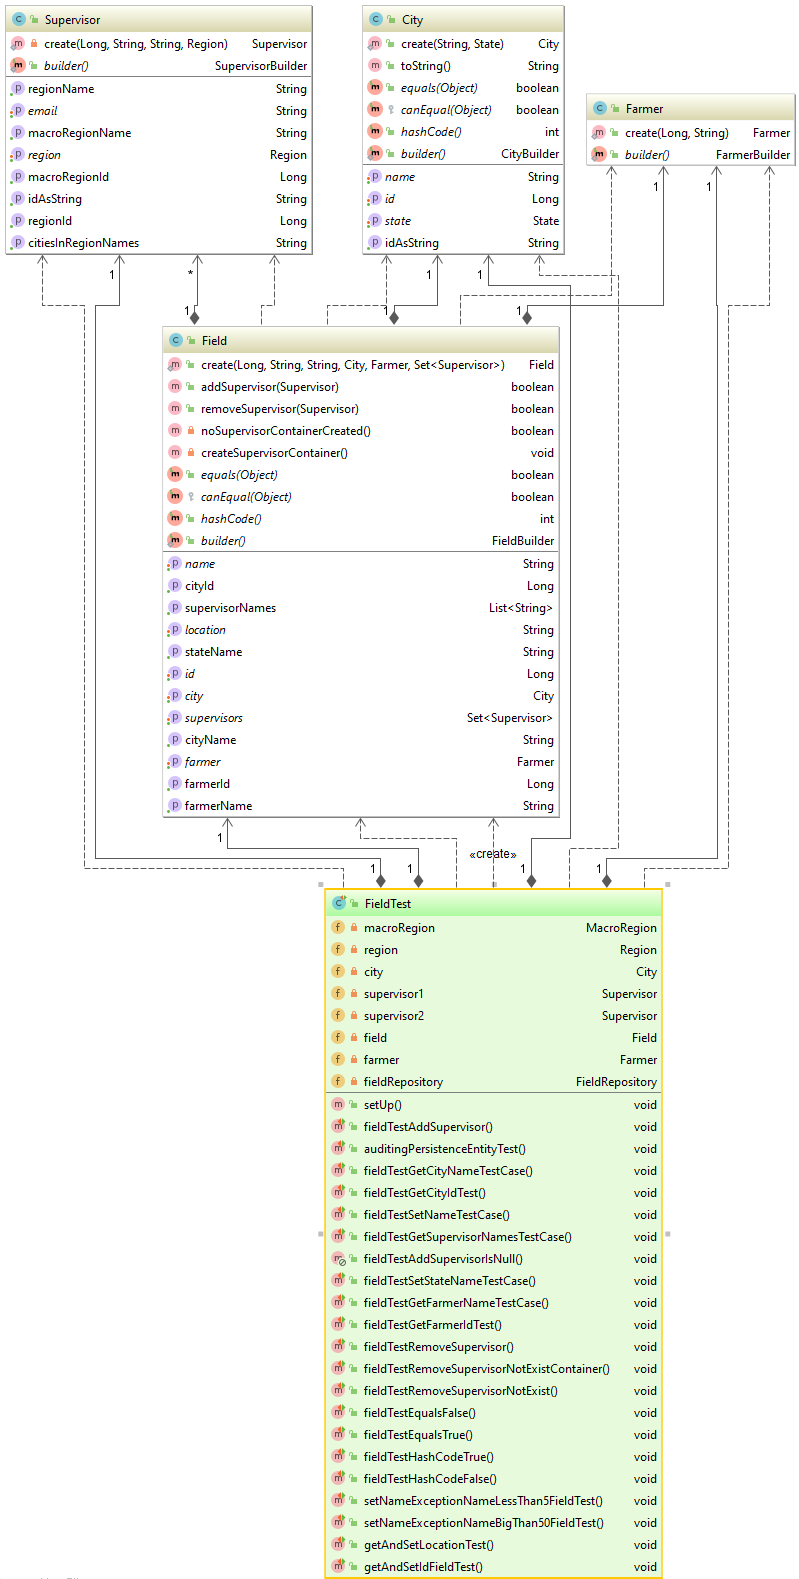
\includegraphics[scale=0.5]{dados/figuras/PackagebaseTestField.png}
	\caption{Diagrama de classes FieldServiceTest.java.}
	\label{packFieldService}
\end{figure}

A classe \textit{FieldService}é responsável por realizar a comunicação com a classe \textit{Field}, e com as demais classes que a compõem. A FIGURA \ref{packFieldService} apresenta o diagrama de classes da classe \textit{FieldService}e as demais classes que a compõem assim como a classe responsável por realizar os testes de seus métodos e variáveis. Também é possível analisar no diagrama os atributos e métodos que pertence à classe \textit{ FieldService }, assim como os métodos e atributos da classe de \textit{ FieldServiceTest}.  


A classe de teste apresentada na FIGURA \ref{packFieldService} possui vinte e três métodos de teste é um método de apoio aos testes denominado \textit{“setUp”}, o objetivo dos testes é exercitar a classe \textit{FieldService} até que todos as variáveis, entradas e saídas de dados sejam executados pelo menos uma vez. Como a classe \textit{FieldService} trabalha com outras classes além da \textit{Field} se faz necessário a instanciação destas como: \textit{Supervisor}, \textit{Farmer}, \textit{City} e outras para a execução completa dos testes. Como a classe trabalha com entidades que serão persistidas em um banco de dados, foi preciso criar uma referência para a interface \textit{FieldRepository} e outros repositórios que são chamados durante a execução dos testes. Como o objetivo deste trabalho é cobrir o sistema com testes unitários e testes que integram classes entidades com o banco de dados ou comunicação com APIs são testes de integração foi utilizado\textit{ “Mocks”} para simular o comportamento dos repositórios.



A FIGURA \ref{testeFieldService} apresenta a declaração da classe de teste, os atributos utilizados para desenvolver os testes e o método\textit{ “setUp”} utilizado para preparar o ambiente para os teste.

O trecho de código da FIGURA \ref{testeFieldService} apresenta as seguintes funcionalidades:

\begin{itemize}
\item Linha 1 A anotação \textit{@RunWith} permite a execução dos testes dentro de um contexto do \textit{Spring}. O comando \textit{SpringRunner}.class fornece suporte para carregar um \textit{Spring} \textit{ApplicationContext} e ter \textit{beans }\textit{@Autowired} na instância de teste.
\item Na linha 2 é utilizada a anotação \textit{@SpringBootTest} que prepara um contexto \textit{Spring} e inclui a possibilidade de iniciar um container em um porta default ou configurada pelo usuário. Neste caso a porta foi definida de forma randômica através do comando \textit{“SpringBootTest.WebEnvironment.RANDOM\_PORT”}; 

 \item Na linha 3 é utilizada a anotação \textit{@FixMethodOrder} que permite definir uma ordem de execução dos testes, neste casso foi definida a ordem \textit{“NAME\_ASCENDING"} que faz a execução dos testes de acordo com o nome de maneira ascendente;

 \item Linha 4 a classe \textit{FieldServiceTest} é aberta;

 \item Da linha 6 a 15 há a declaração dos objetos \textit{MOCKs} que serão utilizadas para a comunicação com o banco de dados. A anotação \textit{@MockBean} foi utilizada na declaração destas variáveis, ela permite que caso exista um \textit{bean }compatível com a classe declarada no contexto da aplicação \textit{Spring} este \textit{bean }será substituído por um \textit{Mock};

\item Linhas 14 e 15 uma instancia da classe \textit{FieldService}é declarada, a anotação \textit{@Autowired} é utilizada para a injeção automática de um \textit{bean }correspondente ao declarado na variável.
 
\item Da linha 17 a 21 há a declaração dos objetos que serão utilizados nos testes;

 



\item Na linha 24 é utilizado a anotação \textit{@Before}, esta anotação determina que sempre antes da execução de um teste o método \textit{“setUp”} deve ser executado primeiro.


\begin{figure}[H]
	\centering
	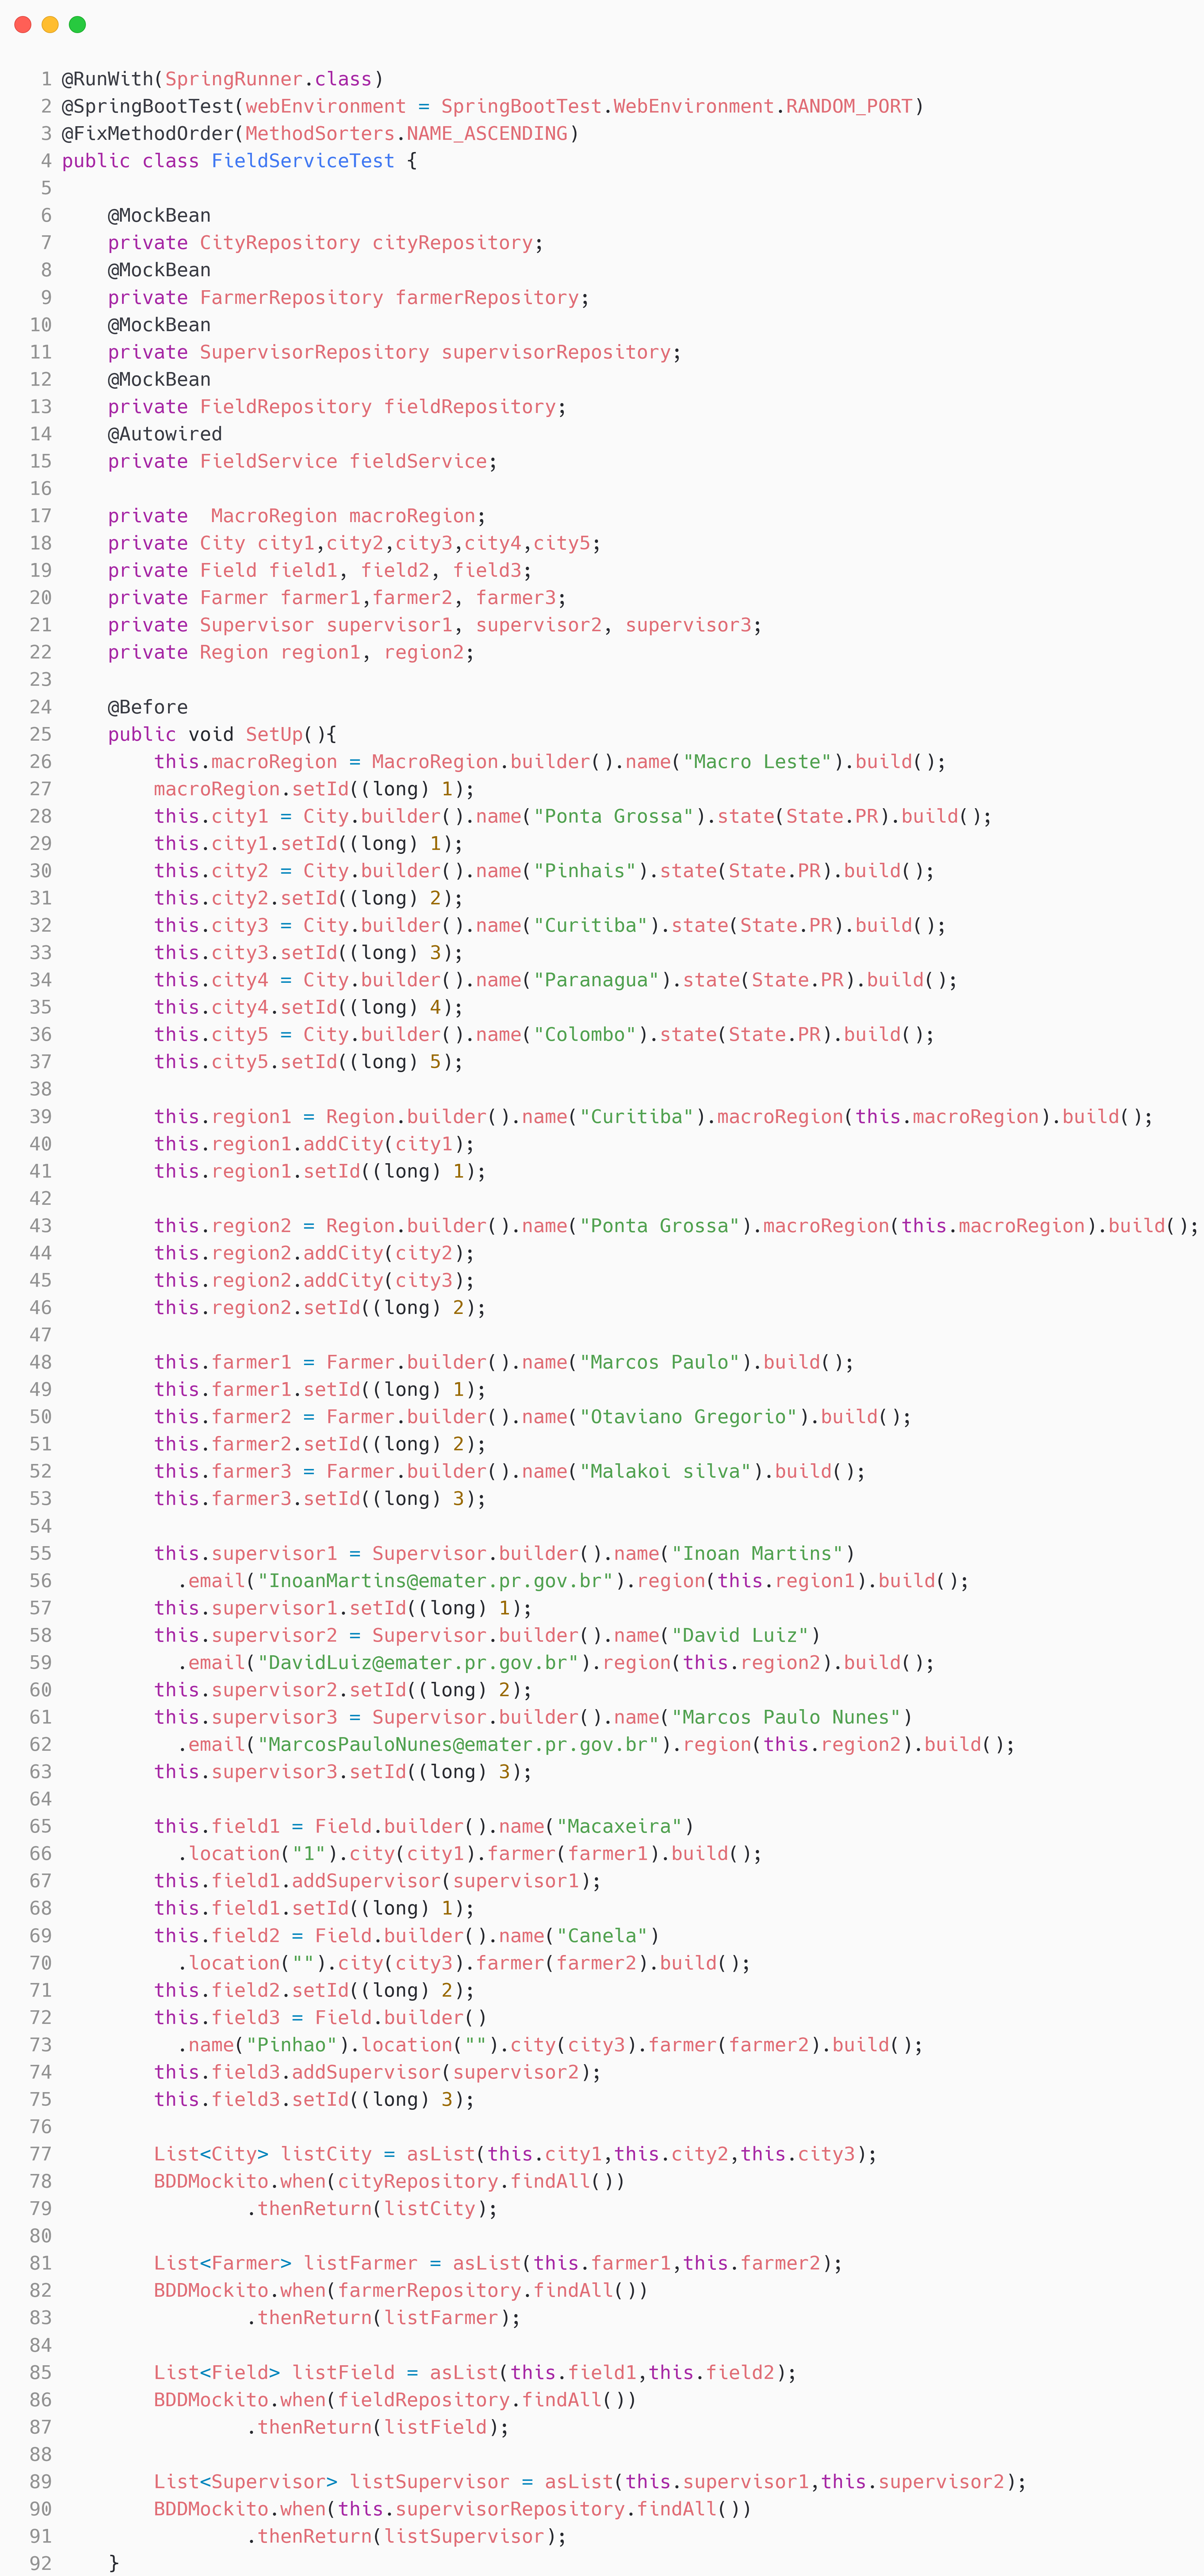
\includegraphics[scale=0.13]{dados/figuras/carbonFieldServicebuild.png}
\end{figure}

\begin{figure}[H]
	\centering
	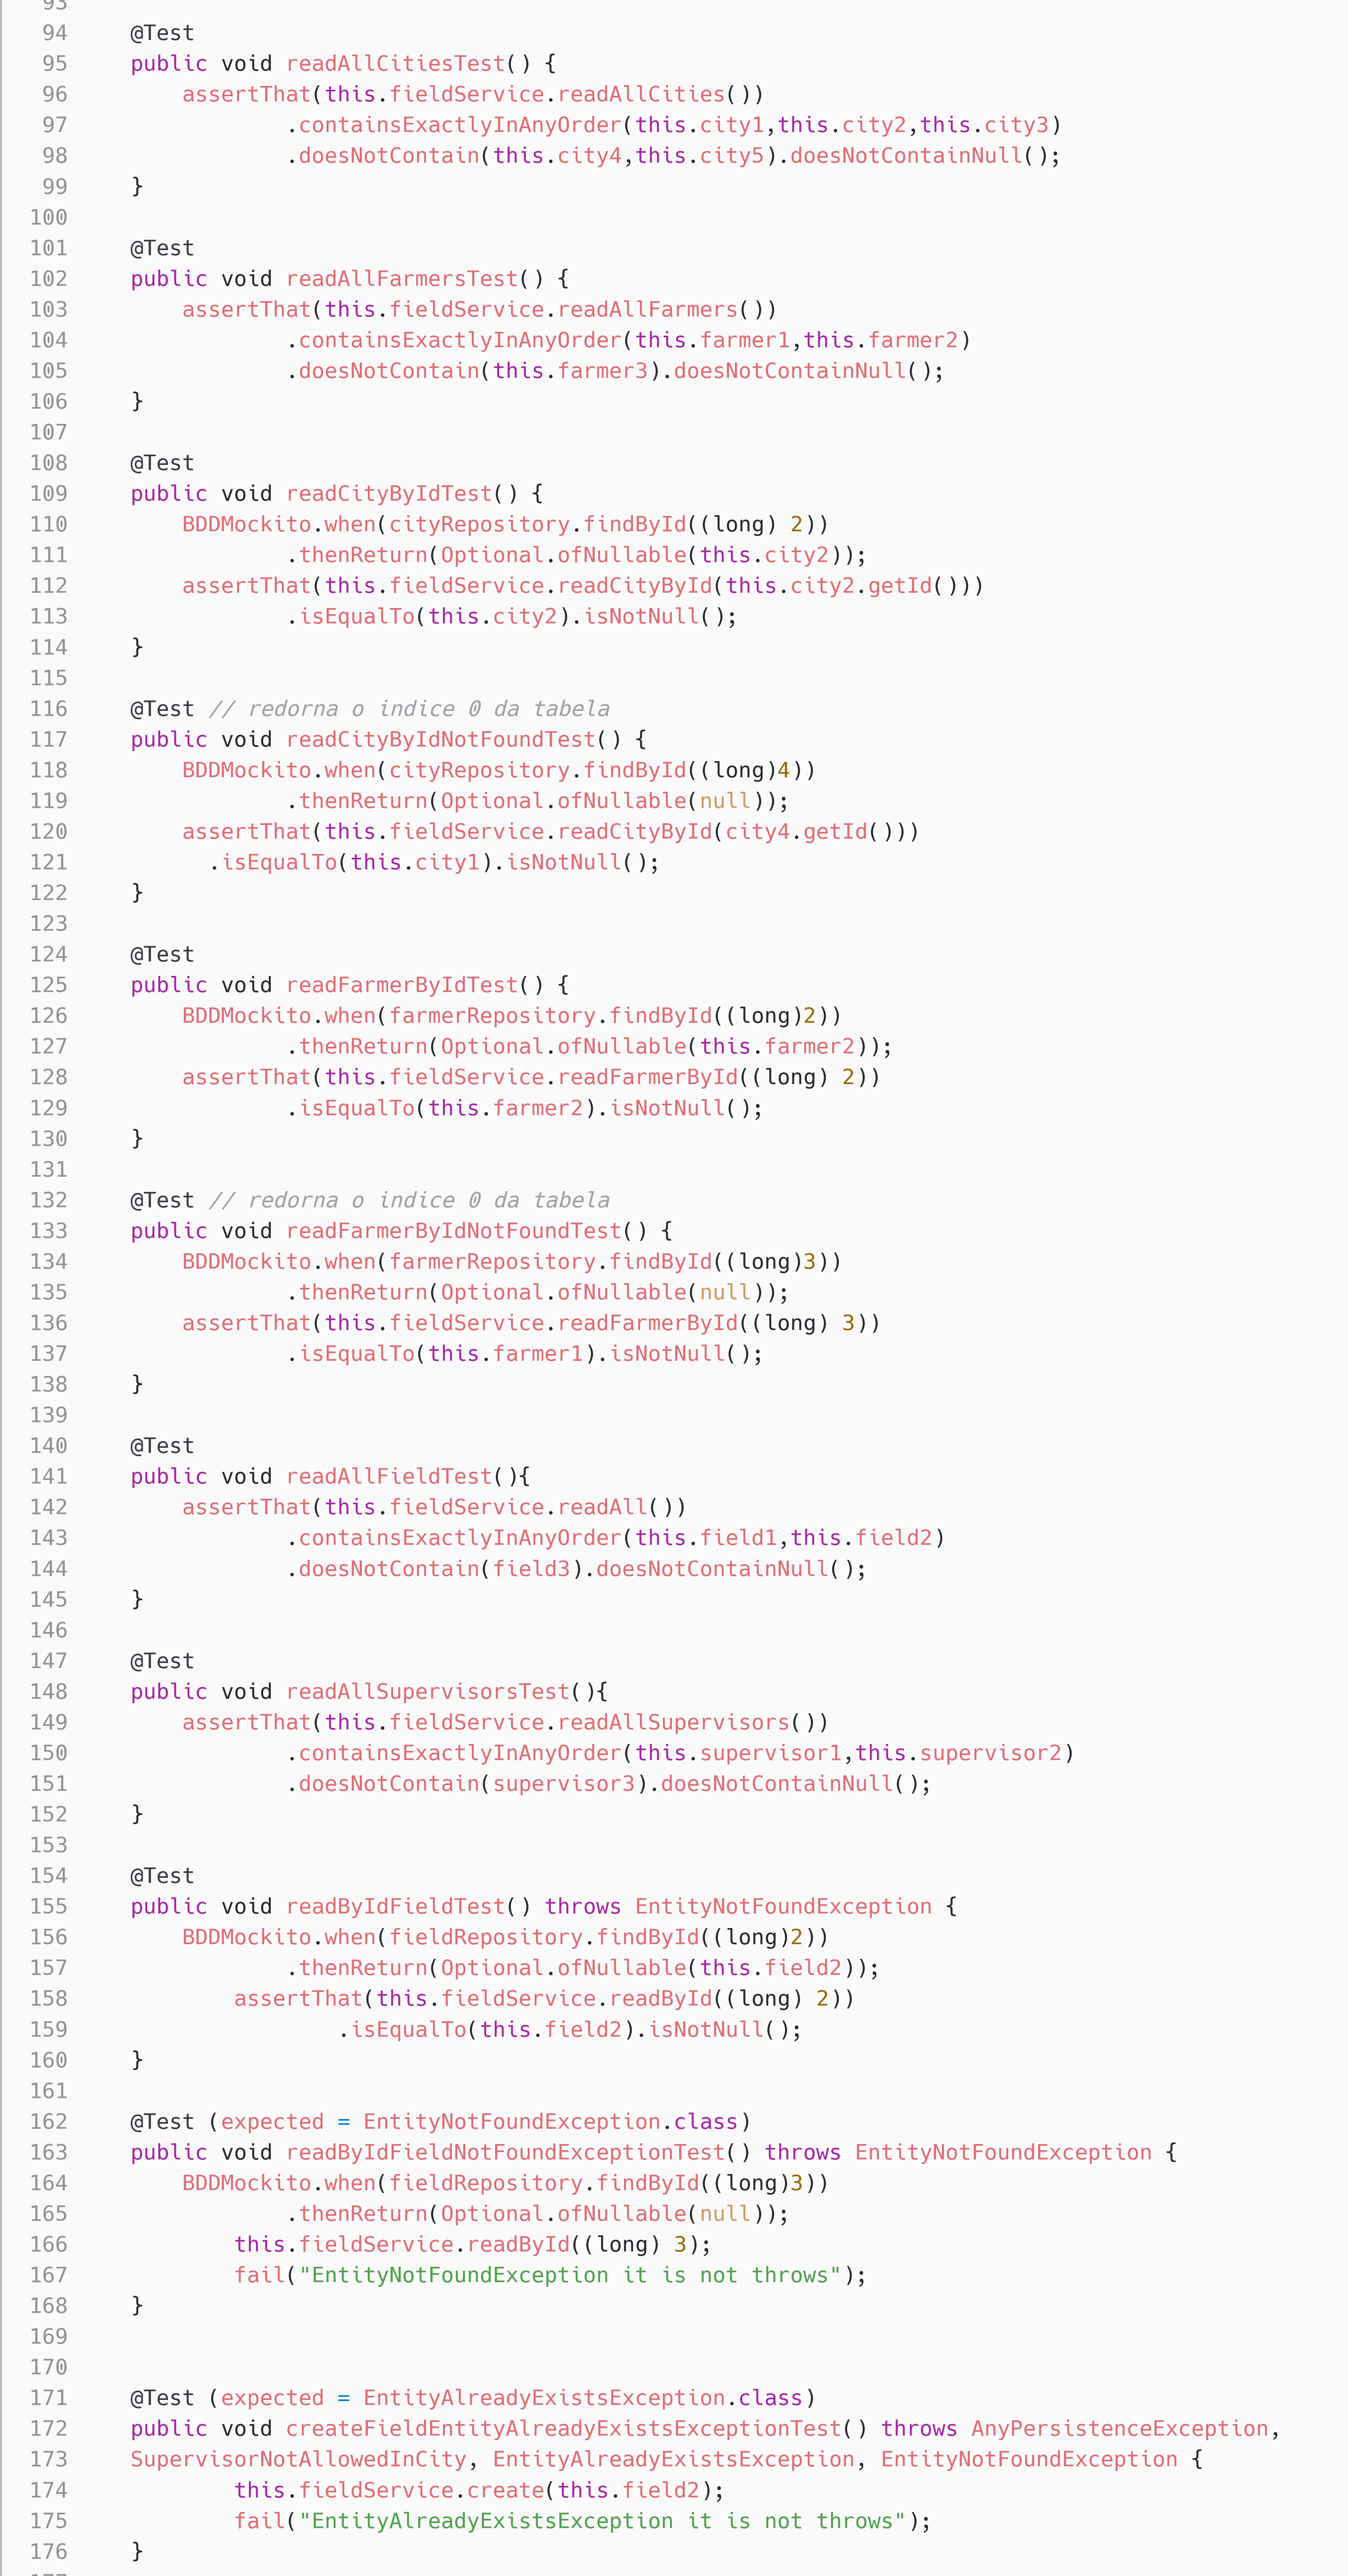
\includegraphics[scale=0.14]{dados/figuras/carbonFieldService1.png}
\end{figure}

\begin{figure}[H]
	\centering
	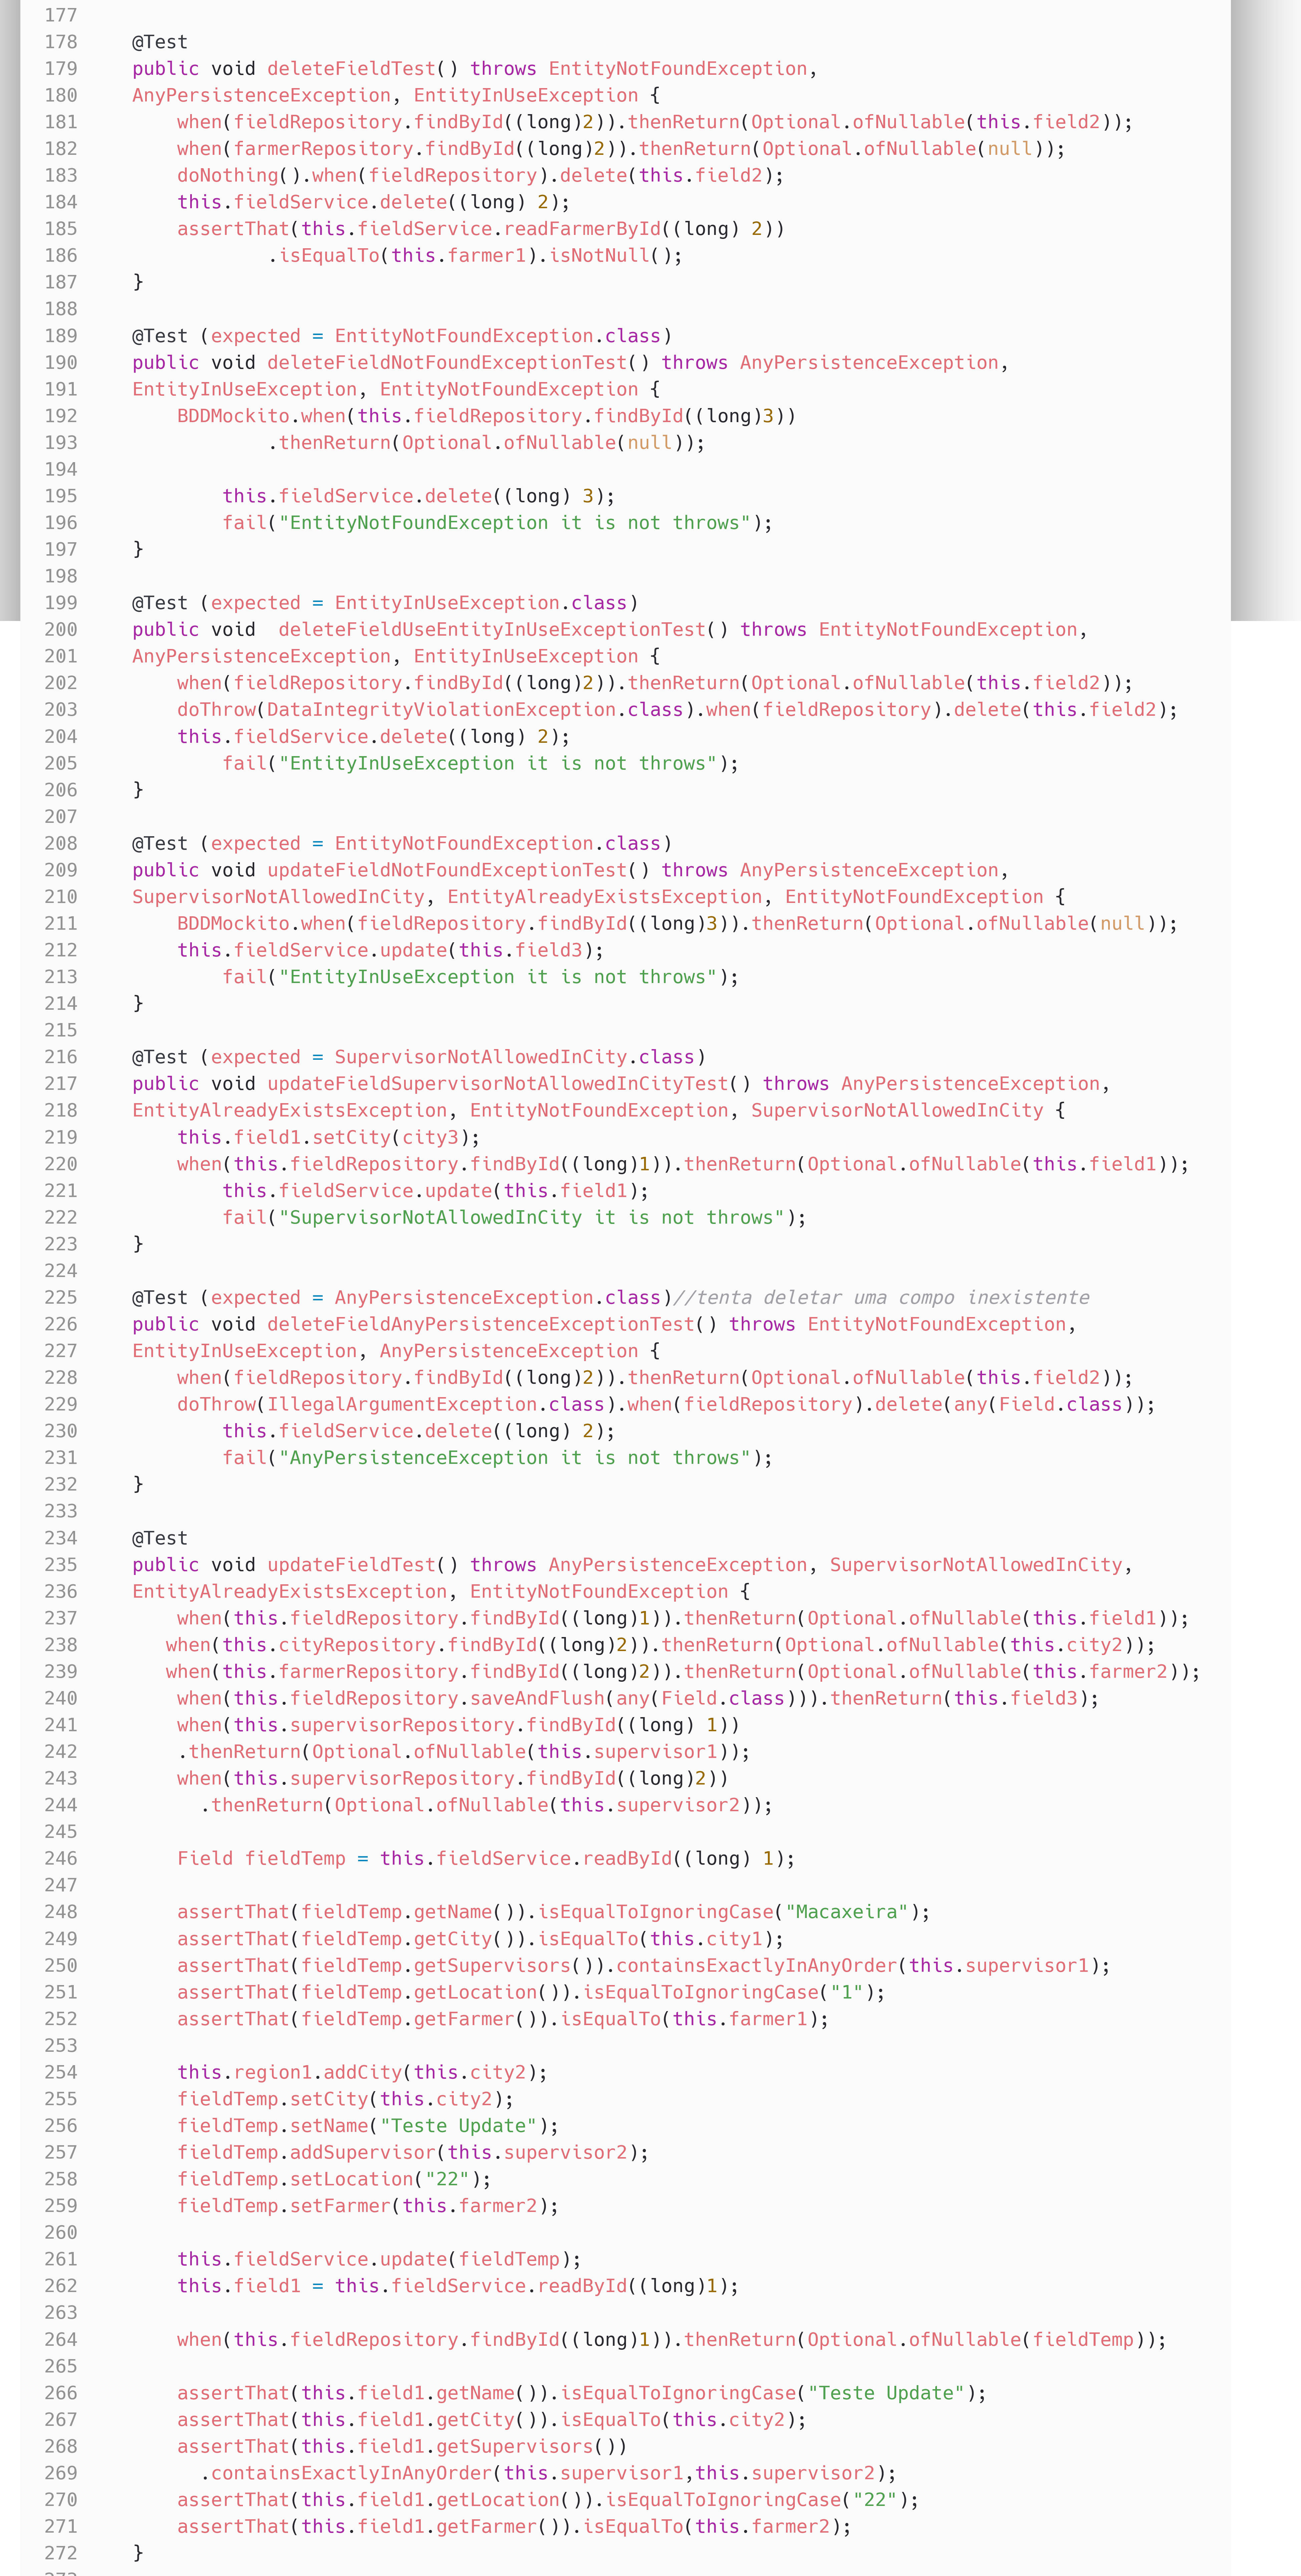
\includegraphics[scale=0.13]{dados/figuras/carbonFieldService2.png}
\end{figure}

\begin{figure}[H]
	\centering
	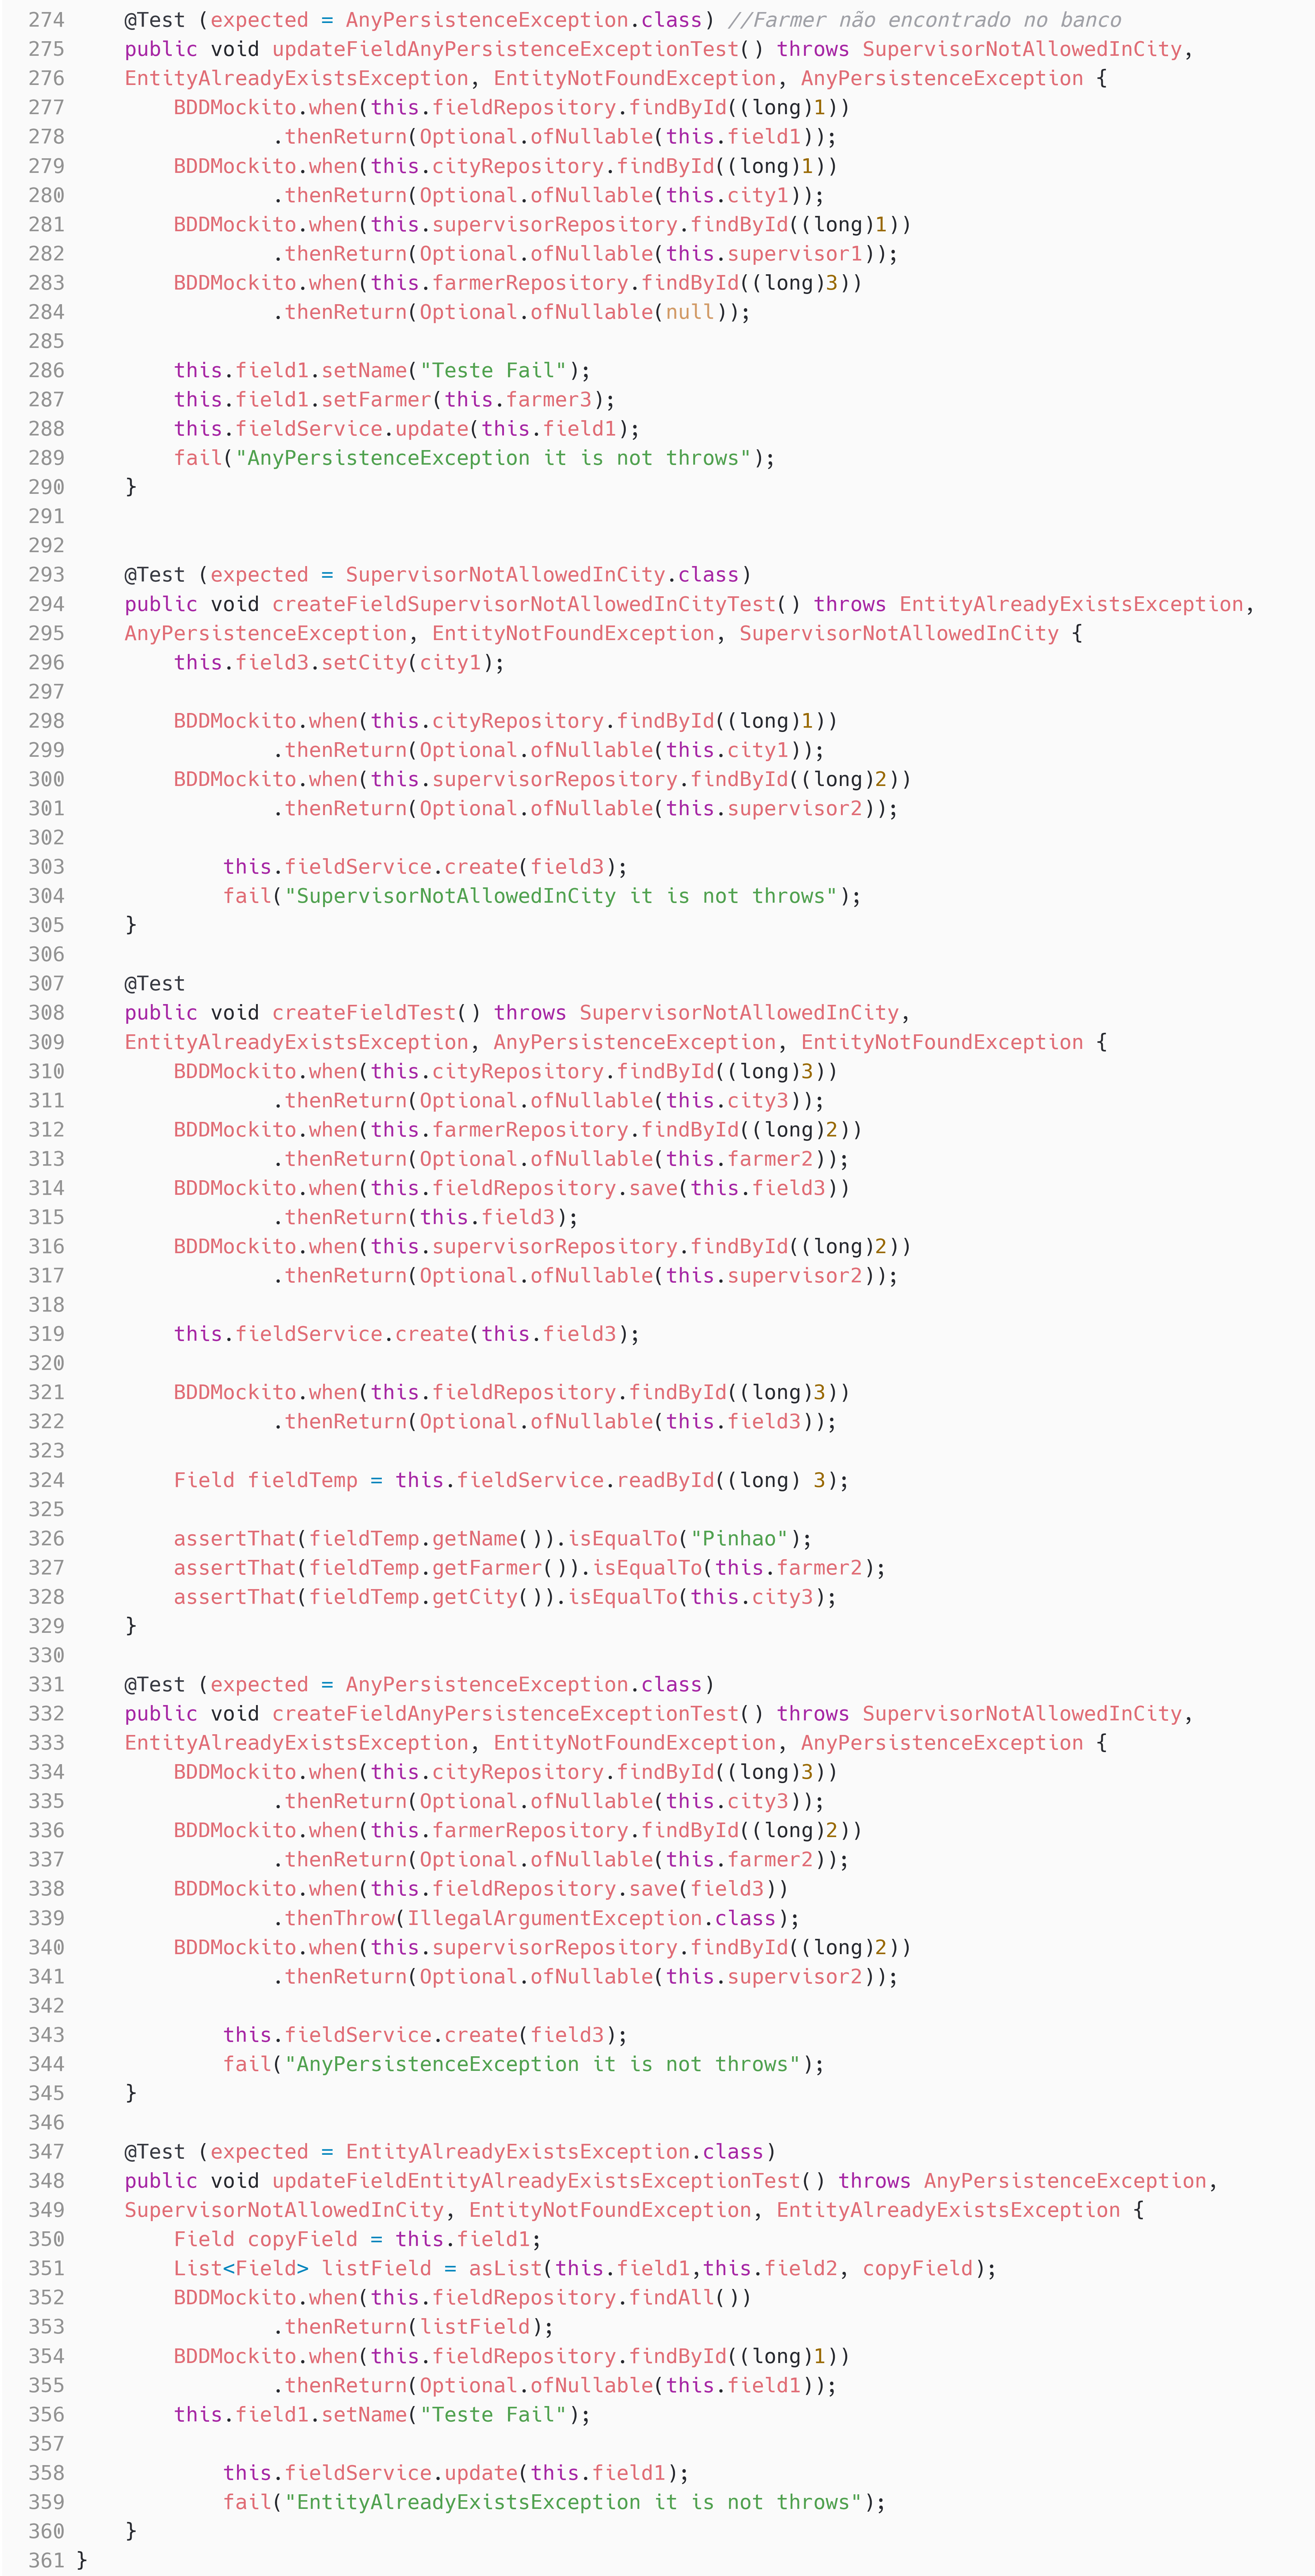
\includegraphics[scale=0.13]{dados/figuras/carbonFieldService3.png}
	\caption{Classe de Teste  FieldService.java.}
	\label{testeFieldService}
\end{figure}

 \item O método \textit{“setUp”} que tem sua declaração na linha 25 e vai até a linha 92 é responsável por realizar a construção dos objetos declarados nas linhas 17 a 21.

\item O método  \textit{“setUp”} também é responsável por construir algumas funcionalidades para os objetos do tipo Mock:

\begin{itemize}

 \item Linha  78 é definido que toda vez que o comando \textit{“cityRepository.findAll()”} for chamado o retorno será uma lista do tipo “\textit{City}” definida na linha 77;
\item Linha  82 é definido que toda vez que o comando \textit{“farmerRepository.findAll()”} for chamado o retorno será uma lista do tipo “\textit{Farmer}” definida na linha 81;
\item Linha  86 é definido que toda vez que o comando \textit{“fieldRepository.findAll()”} for chamado o retorno será uma lista do tipo \textit{Field} definida na linha 85;
\item Linha  90 é definido que toda vez que o comando\textit{ “supervisorRepository.findAll()”} for chamado o retorno será uma lista do tipo “\textit{City}” definida na linha 89;
\end{itemize}{}
\end{itemize}{}


A FIGURA \ref{testeFieldService} tambem apresenta os casos de testes criados para a classe \textit{FieldTest}. 


A ideia geral na elaboração dos testes é a de cobrir cada atribuição de dados, as entrada e saída de dados da classe \textit{FieldService}, buscando a cobertura de 100\% das linhas métodos e atributo da classe. Os resultados obtidos da execução dos testes foram listados a seguir:


Método de teste \textit{readAllCitiesTest ()} linhas 94 a 99 figura \ref{testeFieldService}: Este teste lista todas as cidades do banco de dados. Não há entrada de dados. A Saída é uma lista do tipo \textit{“City”} contendo as cidades salvas na base de dados. Nesta assertiva o método testado deve retornar a lista criada na linha 77, que contem 3 objetos do tipo cidade correspondentes a comparação.

Método de teste \textit{ readAllFarmersTest ()} linhas 101 a 106 figura \ref{testeFieldService}: Este teste lista todos os agricultores do banco de dados. Não há entrada de dados. A Saída é uma lista do tipo \textit{“Farmer”} contendo agricultores salvos na base de dados. Nesta assertiva o método testado deve retornar a lista criada na linha 81, que contem 2 objetos do tipo agricultor correspondentes a comparação.

Método de teste \textit{ readCityByIdTest ()} linhas 108 a 114 figura \ref{testeFieldService}: Este teste busca uma cidade na base de dados pelo seu identificador único. A entrada consiste em um numeral do tipo \textit{“Long”}. A saída é um objeto do tipo \textit{“City”}. Nesta assertiva o método testado deve retornar o registro \textit{mocado} nas linhas 110 e 111, o qual corresponde ao objeto comparado. 

Método de teste \textit{ readCityByIdNotFoundTest ()} linhas 116 a 122 figura \ref{testeFieldService}: Este teste busca uma cidade na base de dados pelo seu identificador único. A entrada consiste em um numeral do tipo \textit{“Long”}. A saída é um objeto do tipo \textit{“City”}. Nesta assertiva o método testado deve retornar o índice zero da lista criada na linha 77, o qual corresponde ao objeto comparado.

Método de teste \textit{ readFarmerByIdTest ()} linhas 124 a 130 figura \ref{testeFieldService}: Este teste busca um agricultor na base de dados pelo seu identificador único. A entrada consiste em um numeral do tipo \textit{“Long”}. A saída é um objeto do tipo \textit{“Farmer”}. Nesta assertiva o método testado deve retornar o registro \textit{mocado} nas linhas 126 e 127, o qual corresponde ao objeto comparado.

Método de teste \textit{ readFarmerByIdNotFoundTest ()} linhas 132 a 138 figura \ref{testeFieldService}: Este teste busca um agricultor na base de dados pelo seu identificador único. A entrada consiste em um numeral do tipo \textit{“Long”}. A saída é um objeto do tipo \textit{“Farmer”}. Nesta assertiva o método testado deve retornar o índice zero da lista criada na linha 81, o qual corresponde ao objeto comparado.


Método de teste \textit{ readAllFieldTest ()} linhas 140 a 145 figura \ref{testeFieldService}: Este teste busca os registros do tipo \textit{Field} na base de dados. Não há entrada de dados.  A saída é uma lista do tipo \textit{Field}. Nesta assertiva o método testado deve retornar a lista criada na linha 85, que contem dois registros correspondentes a comparação.

Método de teste \textit{readAllSupervisorsTest ()} linhas 147 a 152 figura \ref{testeFieldService}: Este teste busca os registros do tipo \textit{“Supervisor”} na base de dados. Não há entrada de dados.  A saída é uma lista do tipo \textit{“Supervisor”}. Nesta assertiva o método testado deve retornar a lista criada na linha 89, que contém dois registros correspondentes a comparação.

Método de teste \textit{ readByIdFieldTest ()} linhas 154 a 160 figura \ref{testeFieldService}: Este teste busca um registro do tipo \textit{Field} na base de dados pelo seu identificador único. A entrada consiste em um numeral do tipo \textit{“Long”}. A saída é um objeto do tipo \textit{Field}. Nesta assertiva o método testado deve retornar o objeto \textit{mocado} nas linhas 156 e 157, o qual corresponde ao objeto comparado.

Método de teste \textit{ readByIdFieldNotFoundExceptionTest ()} linhas 162 a 168 figura \ref{testeFieldService}: Este teste busca um registro do tipo \textit{Field} na base de dados pelo seu identificador único, quando não encontrado é gerada uma exceção. A entrada consiste em um numeral do tipo \textit{“Long”}. A saída é uma exceção do tipo \textit{“EntityNotFoundException”}. Nesta assertiva o método testado deve retornar uma exceção, ao buscar um objeto pelo índice passado como parâmetro, ao realizar a consulta no banco um registro vazio é retornado, o que é simulado nas linhas 164 e 165, o que garante o lançamento da exceção \textit{“EntityNotFoundException”}.


Método de teste \textit{ createFieldEntityAlreadyExistsExceptionTest ()} linhas 171 a 176 figura \ref{testeFieldService}:  Este teste consiste em tentar criar um novo registro do tipo \textit{Field}, mas o item a ser criado é identificado como já existente na base de dados. A Entrada consiste em um objeto do tipo \textit{Field}. A Saída é o lançamento da exceção \textit{“EntityAlreadyExistsException”}. A assertiva tenta inserir um registro que já se encontra na base de dados simulada pela linha 85, o que proporciona o lançamento da exceção.  

Método de teste \textit{ deleteFieldTest ()} linhas 178 a 187 figura \ref{testeFieldService}: Este teste consiste em deletar um registro do tipo \textit{Field}. A Entrada consiste em um objeto do tipo \textit{Field}. Não há saída de dados.  A assertiva deleta um registro do banco linha 183, a validação é feita ao tentar consultar por este registro no banco simulado, o retorno é o índice zero do banco e não o procurado.  

Método de teste \textit{ deleteFieldNotFoundExceptionTest ()} linhas 189 a 197 figura \ref{testeFieldService}: Este teste consiste em deletar um registro do tipo \textit{Field}, mas o item a ser deletado não existe na base de dados. A Entrada consiste em um objeto do tipo \textit{Field}. A Saída é o lançamento da exceção \textit{“EntityNotFoundException”}. A assertiva tenta deletar um registro, mas ao consultar o registro na base de dados simulada pela linha 192 o retorno é um nulo pois ele não existe na base, há o lançamento da exceção.  

Método de teste \textit{ deleteFieldUseEntityInUseExceptionTest ()} linhas 199 a 206 figura \ref{testeFieldService}: Este teste consiste em deletar um registro do tipo \textit{Field}, mas o item a ser deletado está sendo utilizado na base de dados. A Entrada consiste em um objeto do tipo \textit{Field}. A Saída é o lançamento da exceção \textit{“UseEntityInUseException”}. A assertiva tenta deletar um registro, mas este está sendo utilizado na base de dados simulada pela linha 203, há o lançamento da exceção.  

Método de teste \textit{ updateFieldNotFoundExceptionTest ()} linhas 208 a 214 figura \ref{testeFieldService}: Este teste consiste em atualizar um registro do tipo \textit{Field}, mas o item a ser atualizado não existe na base de dados. A Entrada consiste em um objeto do tipo \textit{Field}. A Saída é o lançamento da exceção \textit{“EntityNotFoundException”}. A assertiva tenta atualizar um registro, mas ao consultar o registro na base de dados simulada pela linha 211 o retorno é um nulo pois ele não existe na base, há o lançamento da exceção.  

Método de teste \textit{ updateFieldSupervisorNotAllowedInCityTest ()} linhas 216 a 223 figura \ref{testeFieldService}: Este teste consiste em tentar atualizar um registro do tipo \textit{Field}, mas é identificado que os supervisores presentes no registro não pertencem a cidade que compõe o registro. A Entrada consiste em um objeto do tipo \textit{Field}. A Saída é o lançamento da exceção \textit{“SupervisorNotAllowedInCity”}. A assertiva tenta atualizar um registro que possui supervisores que não se localizam na cidade do registro linha 219, o que proporciona o lançamento da exceção.  


Método de teste \textit{ deleteFieldAnyPersistenceExceptionTest ()} linhas 225 a 232 figura \ref{testeFieldService}: Este teste consiste em deletar um registro do tipo \textit{Field}, mas o item a ser deletado gera um erro na base de dados. A Entrada consiste em um objeto do tipo \textit{Field}. A Saída é o lançamento da exceção \textit{“AnyPersistenceException”}. A assertiva tenta deletar um registro, mas um erro é gerado, há o lançamento da exceção.  

Método de teste \textit{ updateFieldTest ()} linhas 234 a 272 figura \ref{testeFieldService}: Este teste consiste em atualizar um registro do tipo \textit{Field}. A Entrada consiste em um objeto do tipo \textit{Field}. Não há saída de dados. As assertivas consistem em recuperar um objeto da base de dados simulada linha 237, atualizar os campos deste objeto linhas 254 a 259, e em seguida atualizar esse registro na base linha 240. Caso não haja o lançamento de uma exceção o objeto atualizado é recuperado da base simulada, linha 264, e em seguida é feita as assertivas dos dados atualizados.

Método de teste \textit{ updateFieldAnyPersistenceExceptionTest ()} linhas 274 a 290 figura \ref{testeFieldService}: Este teste consiste em atualizar um registro do tipo \textit{Field}, mas o item a ser atualizado possui um agricultor nulo. A Entrada consiste em um objeto do tipo \textit{Field}. A Saída é o lançamento da exceção \textit{“AnyPersistenceException”}. A assertiva tenta atualizar um registro, mas ao consultar o agricultor na base de dados simulada pela linha 283 o retorno é um nulo, há o lançamento da exceção.  

Método de teste \textit{ createFieldSupervisorNotAllowedInCityTest ()} linhas 293 a 305 figura \ref{testeFieldService}: Este teste consiste em tentar criar um novo registro do tipo \textit{Field}, mas é identificado que os supervisores presentes no registro não pertencem a cidade que compõe o registro. A Entrada consiste em um objeto do tipo \textit{Field}. A Saída é o lançamento da exceção \textit{“SupervisorNotAllowedInCity”}. A assertiva tenta inserir um registro que possui supervisores que não se localizam na cidade do registro linha 296, o que proporciona o lançamento da exceção.  

Método de teste \textit{ createFieldTest ()} linhas 307 a 329 figura \ref{testeFieldService}: Este teste consiste em criar um novo registro do tipo \textit{Field} na base de dados. A Entrada consiste em um objeto do tipo \textit{Field}. O método não gera uma saída. A validação é feita através de um \textit{try cath}, que captura qualquer exceção que ocorra ao salvar o objeto. Como o método não lança uma exceção ele é aceito. A assertiva, no entanto, é feita através do repositório \textit{mocado} linhas 321 e 322, depois de inserido é simulada uma consulta pelo identificador único do objeto inserido anteriormente o qual deve retornar o objeto que acaba de ser inserido. 

Método de teste \textit{ createFieldAnyPersistenceExceptionTest ()} linhas 331 a 345 figura \ref{testeFieldService}: Este teste consiste em tentar criar um novo registro do tipo \textit{Field}, mas o item a ser criado gera algum erro na base de dados. A Entrada consiste em um objeto do tipo \textit{Field}. A Saída é o lançamento da exceção \textit{“AnyPersistenceException”}. A assertiva tenta inserir um registro na base de dados simulada pela linha 338, o que proporciona o lançamento da exceção.  

Método de teste \textit{ updateFieldEntityAlreadyExistsExceptionTest ()} linhas 347 a 360 figura \ref{testeFieldService}: Este teste consiste em tentar atualizar um registro do tipo \textit{Field}, mas o item a ser atualizado é identificado como já existente na base de dados. A Entrada consiste em um objeto do tipo \textit{Field}. A Saída é o lançamento da exceção \textit{“EntityAlreadyExistsException”}. A assertiva tenta inserir um registro que já se encontra na base de dados simulada pela linha 351, neste caso foi necessário duplicar o registro a ser atualizado para que o lançamento da exceção fosse forçado.  

Após a execução dos testes a cobertura das entradas e saídas de dados da classe FieldService.java é de 100\%.


 \subsection{RESULTADO DOS TESTES CLASSE SURVEYSERVICE.JAVA}

A classe \textit{SurveyService} é responsável por realizar a comunicação com a classe \textit{Survey}, e com as demais classes que a compõem. A FIGURA \ref{packFieldService} apresenta o diagrama de classes da classe \textit{SurveyService} e as demais classes que a compõem assim como a classe responsável por realizar os testes de seus métodos e variáveis. Também é possível analisar no diagrama os atributos e métodos que pertence à classe \textit{SurveyService}, assim como os métodos e atributos da classe de \textit{SurveyServiceTest}.  


A classe de teste apresentada na FIGURA \ref{packFieldService} possui vinte e quatro métodos de teste é um método de apoio aos testes denominado \textit{“setUp”}, o objetivo dos testes é exercitar a classe \textit{SurveyService} até que todos as variáveis, entradas e saídas de dados sejam executados pelo menos uma vez. Como a classe \textit{SurveyService} trabalha com outras classes além da \textit{Survey} se faz necessário a instanciação destas como: \textit{Supervisor}, \textit{Farmer}, \textit{City} e outras para a execução completa dos testes. Como a classe trabalha com entidades que serão persistidas em um banco de dados, foi preciso criar uma referência para a interface \textit{SurveyRepository} e outros repositórios que são chamados durante a execução dos testes. Como o objetivo deste trabalho é cobrir o sistema com testes unitários e testes que integram classes entidades com o banco de dados ou comunicação com APIs são testes de integração foi utilizado “\textit{MOCKs}” para simular o comportamento dos repositórios.

 \begin{figure}[H]
	\centering
	\includegraphics[scale=0.4]{dados/figuras/PackagesurveyService.png}
	\caption{Diagrama de classes SurveyServiceTest.java.}
	\label{packFieldService}
\end{figure}


A FIGURA \ref{testeSurveyService} apresenta a declaração da classe de teste, os atributos utilizados para desenvolver os testes e o método\textit{ “setUp”} utilizado para preparar o ambiente para os testes.

O trecho de código da FIGURA \ref{testeSurveyService} apresenta as seguintes funcionalidades:


\begin{itemize}

\item Linha 1 A anotação \textit{@RunWith} permite a execução dos testes dentro de um contexto do \textit{Spring}. O comando \textit{SpringRunner}.class fornece suporte para carregar um \textit{Spring}\textit{ApplicationContext} e ter \textit{beans }\textit{@Autowired} na instância de teste.

\item Na linha 2 é utilizada a anotação \textit{@SpringBootTest} que prepara um contexto \textit{Spring} e inclui a possibilidade de iniciar um container em um porta default ou configurada pelo usuário. Neste caso a porta foi definida de forma randômica através do comando \textit{“SpringBootTest.WebEnvironment.RANDOM\_PORT”}; 

 \item Na linha 3 é utilizada a anotação \textit{@FixMethodOrder} que permite definir uma ordem de execução dos testes, neste casso foi definida a ordem \textit{“NAME\_ASCENDING"} que faz a execução dos testes de acordo com o nome de maneira ascendente;

 \item Linha 4 a classe \textit{SurveyServiceTest} é aberta;

 \item Da linha 6 a 11 há a declaração dos objetos \textit{MOCKs} que serão utilizadas para a comunicação com o banco de dados. A anotação \textit{@MockBean} foi utilizada na declaração destas variáveis, ela permite que caso exista um \textit{bean }compatível com a classe declarada no contexto da aplicação \textit{Spring} este \textit{bean }será substituído por um \textit{Mock};

\item Linhas 13 e 14 uma instancia da classe SurveyService é declarada, a anotação \textit{@Autowired} é utilizada para a injeção automática de um \textit{bean }correspondente ao declarado na variável. 
 
\item Da linha 16 a 21 há a declaração dos objetos que serão utilizados nos testes;

 \item Na linha 23 é utilizado a anotação \textit{@Before}, esta anotação determina que sempre antes da execução de um teste o método \textit{“setUp”} deve ser executado primeiro.

 \item O método \textit{“setUp”} que tem sua declaração na linha 24 e vai até a linha 108 é responsável por realizar a construção dos objetos declarados nas linhas 16 a 21.

\item O método  \textit{“setUp”} também é responsável por construir algumas funcionalidades para os objetos do tipo \textit{Mock}:

\begin{itemize}

 \item Linha  107 é definido que toda vez que o comando \textit{“surveyRepository.findAll()”} for chamado o retorno será uma lista do tipo “\textit{Survey}” definida na linha 106;
\end{itemize}{}
\end{itemize}{}


A FIGURA \ref{testeSurveyService} também apresenta os casos de testes criados para a classe \textit{SurveyService}. 


A ideia geral na elaboração dos testes é a de cobrir cada atribuição de dados, as entradas e saída de dados da classe \textit{ SurveyService}, buscando a cobertura de 100\% das linhas métodos e atributo da classe. Os resultados obtidos da execução dos testes foram listados a seguir:


Método de teste \textit{ readAllSurveyTest()} linhas 110 a 115 figura \ref{testeSurveyService}: Este teste lista todas as pesquisas do banco de dados. Não há entrada de dados. A Saída é uma lista do tipo \textit{“Survey”} contendo as pesquisas salvas na base de dados. Nesta assertiva o método testado deve retornar a lista criada na linha 106, que contem 2 objetos do tipo survey correspondentes a comparação.


\begin{figure}[H]
	\centering
	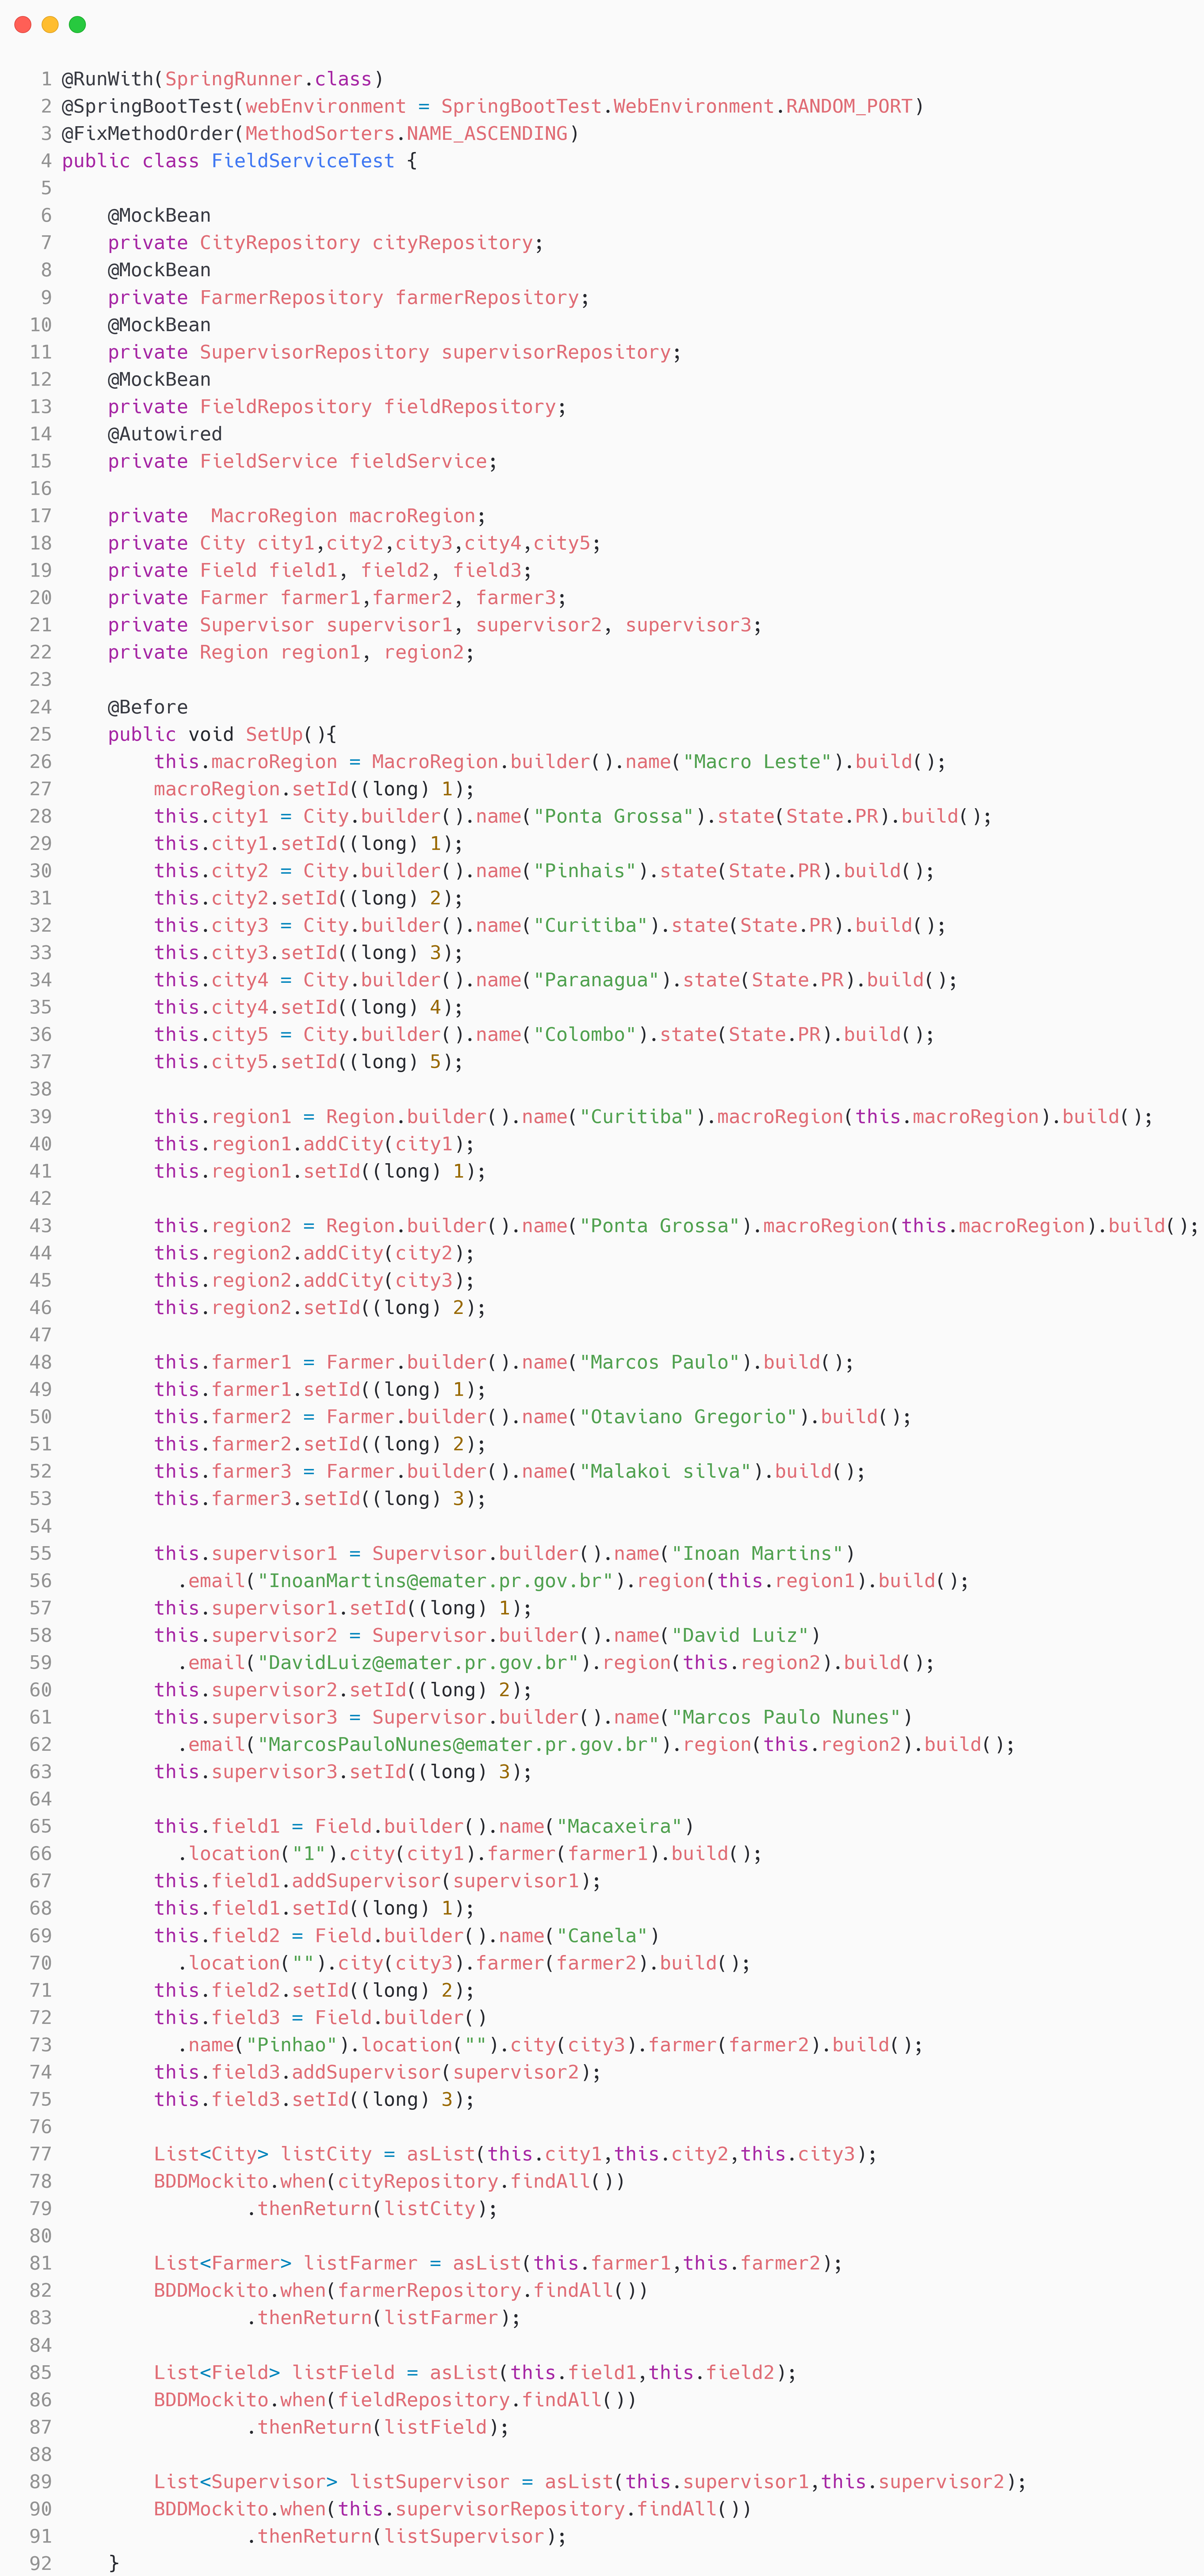
\includegraphics[scale=0.13]{dados/figuras/carbonFieldServicebuild.png}
\end{figure}

\begin{figure}[H]
	\centering
	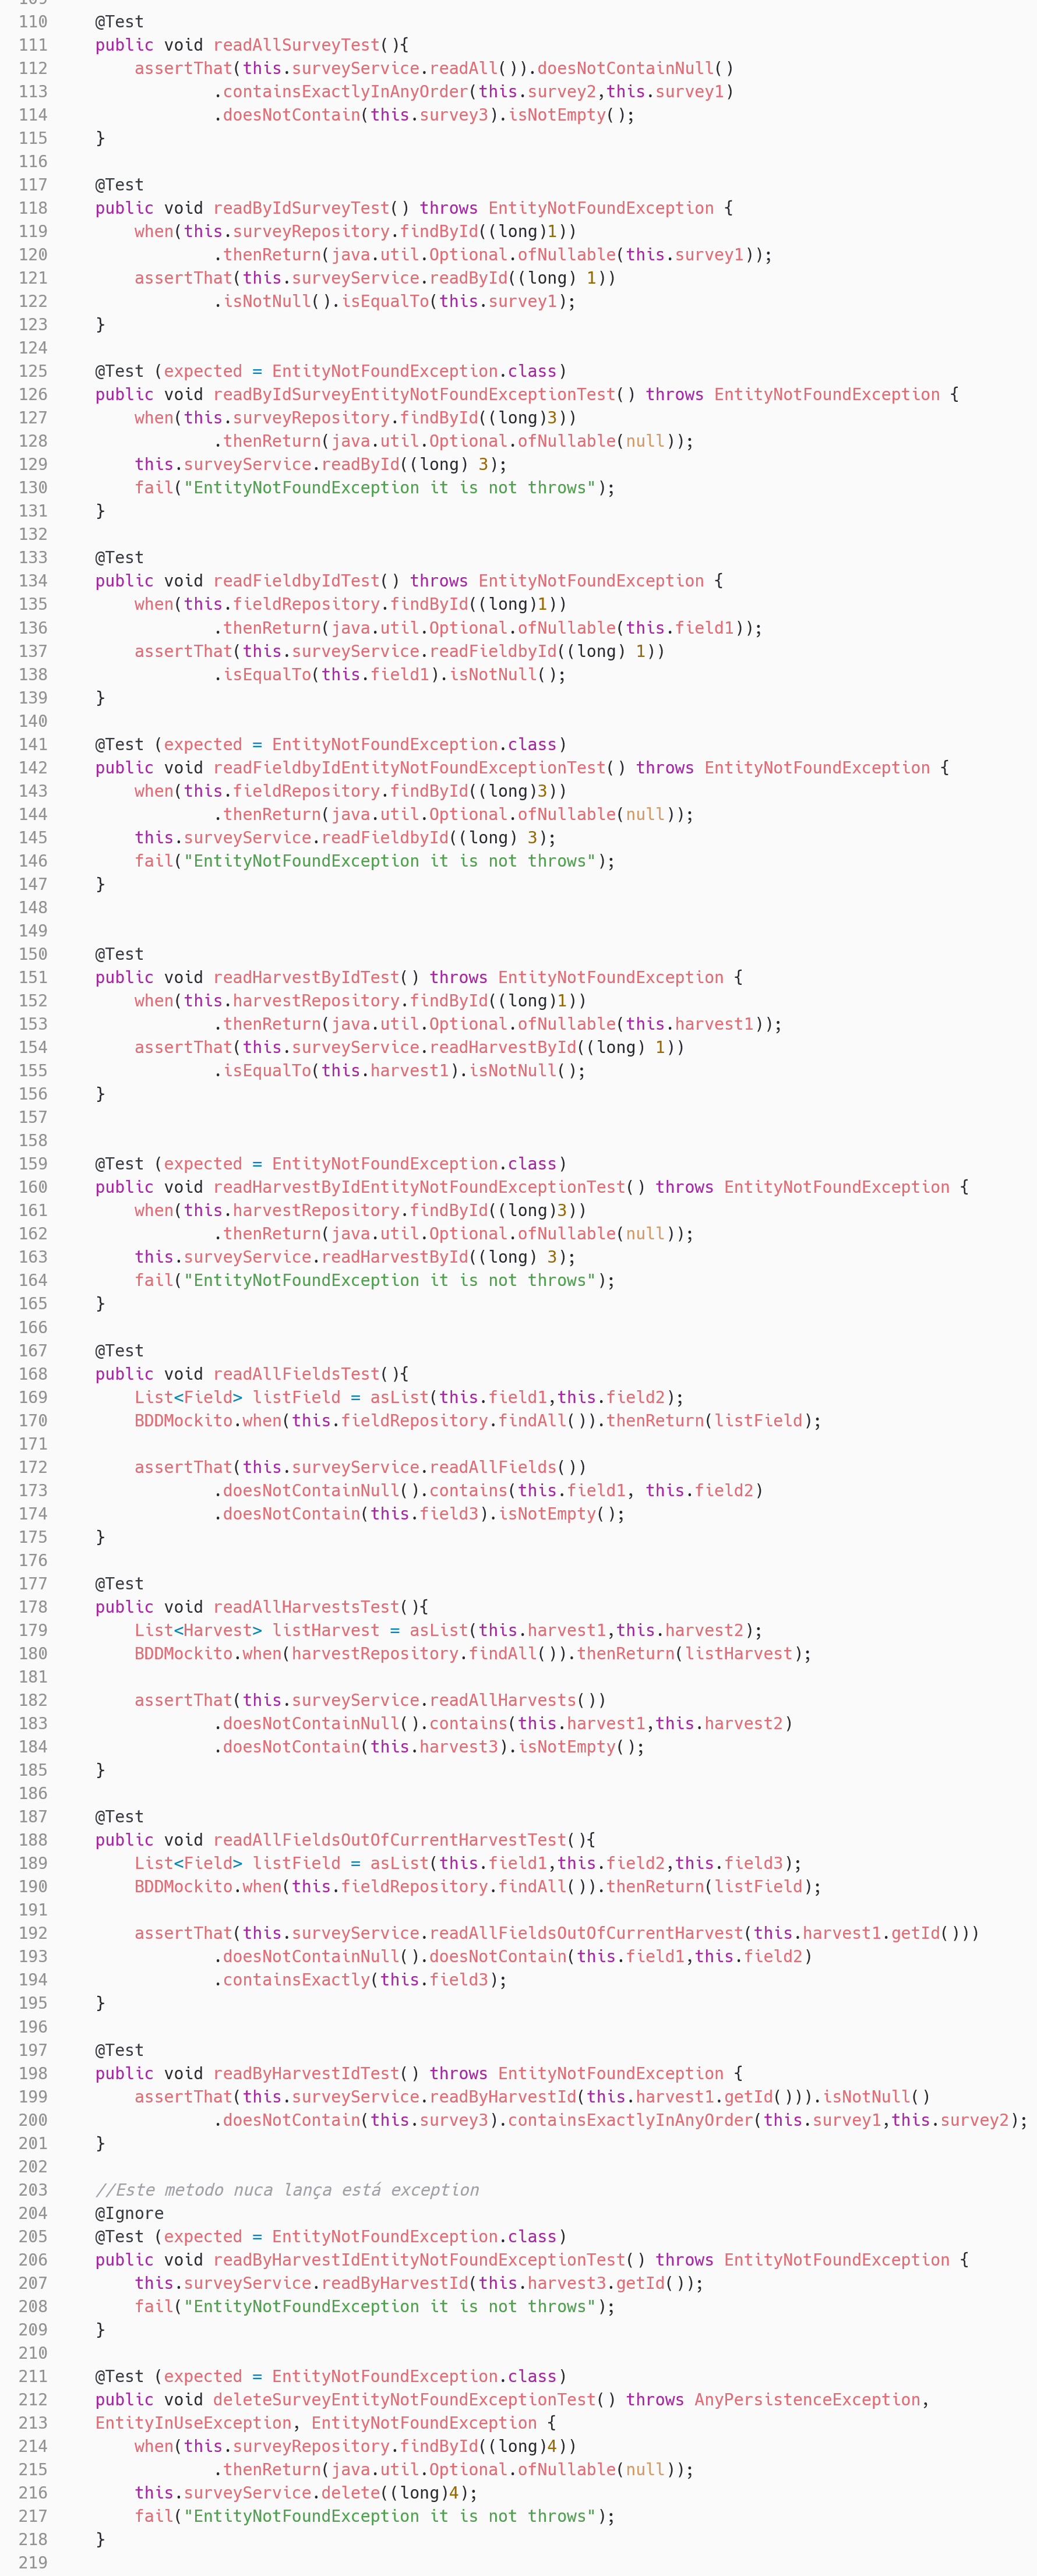
\includegraphics[scale=0.25]{dados/figuras/carbonSurveyService1.png}
\end{figure}

\begin{figure}[H]
	\centering
	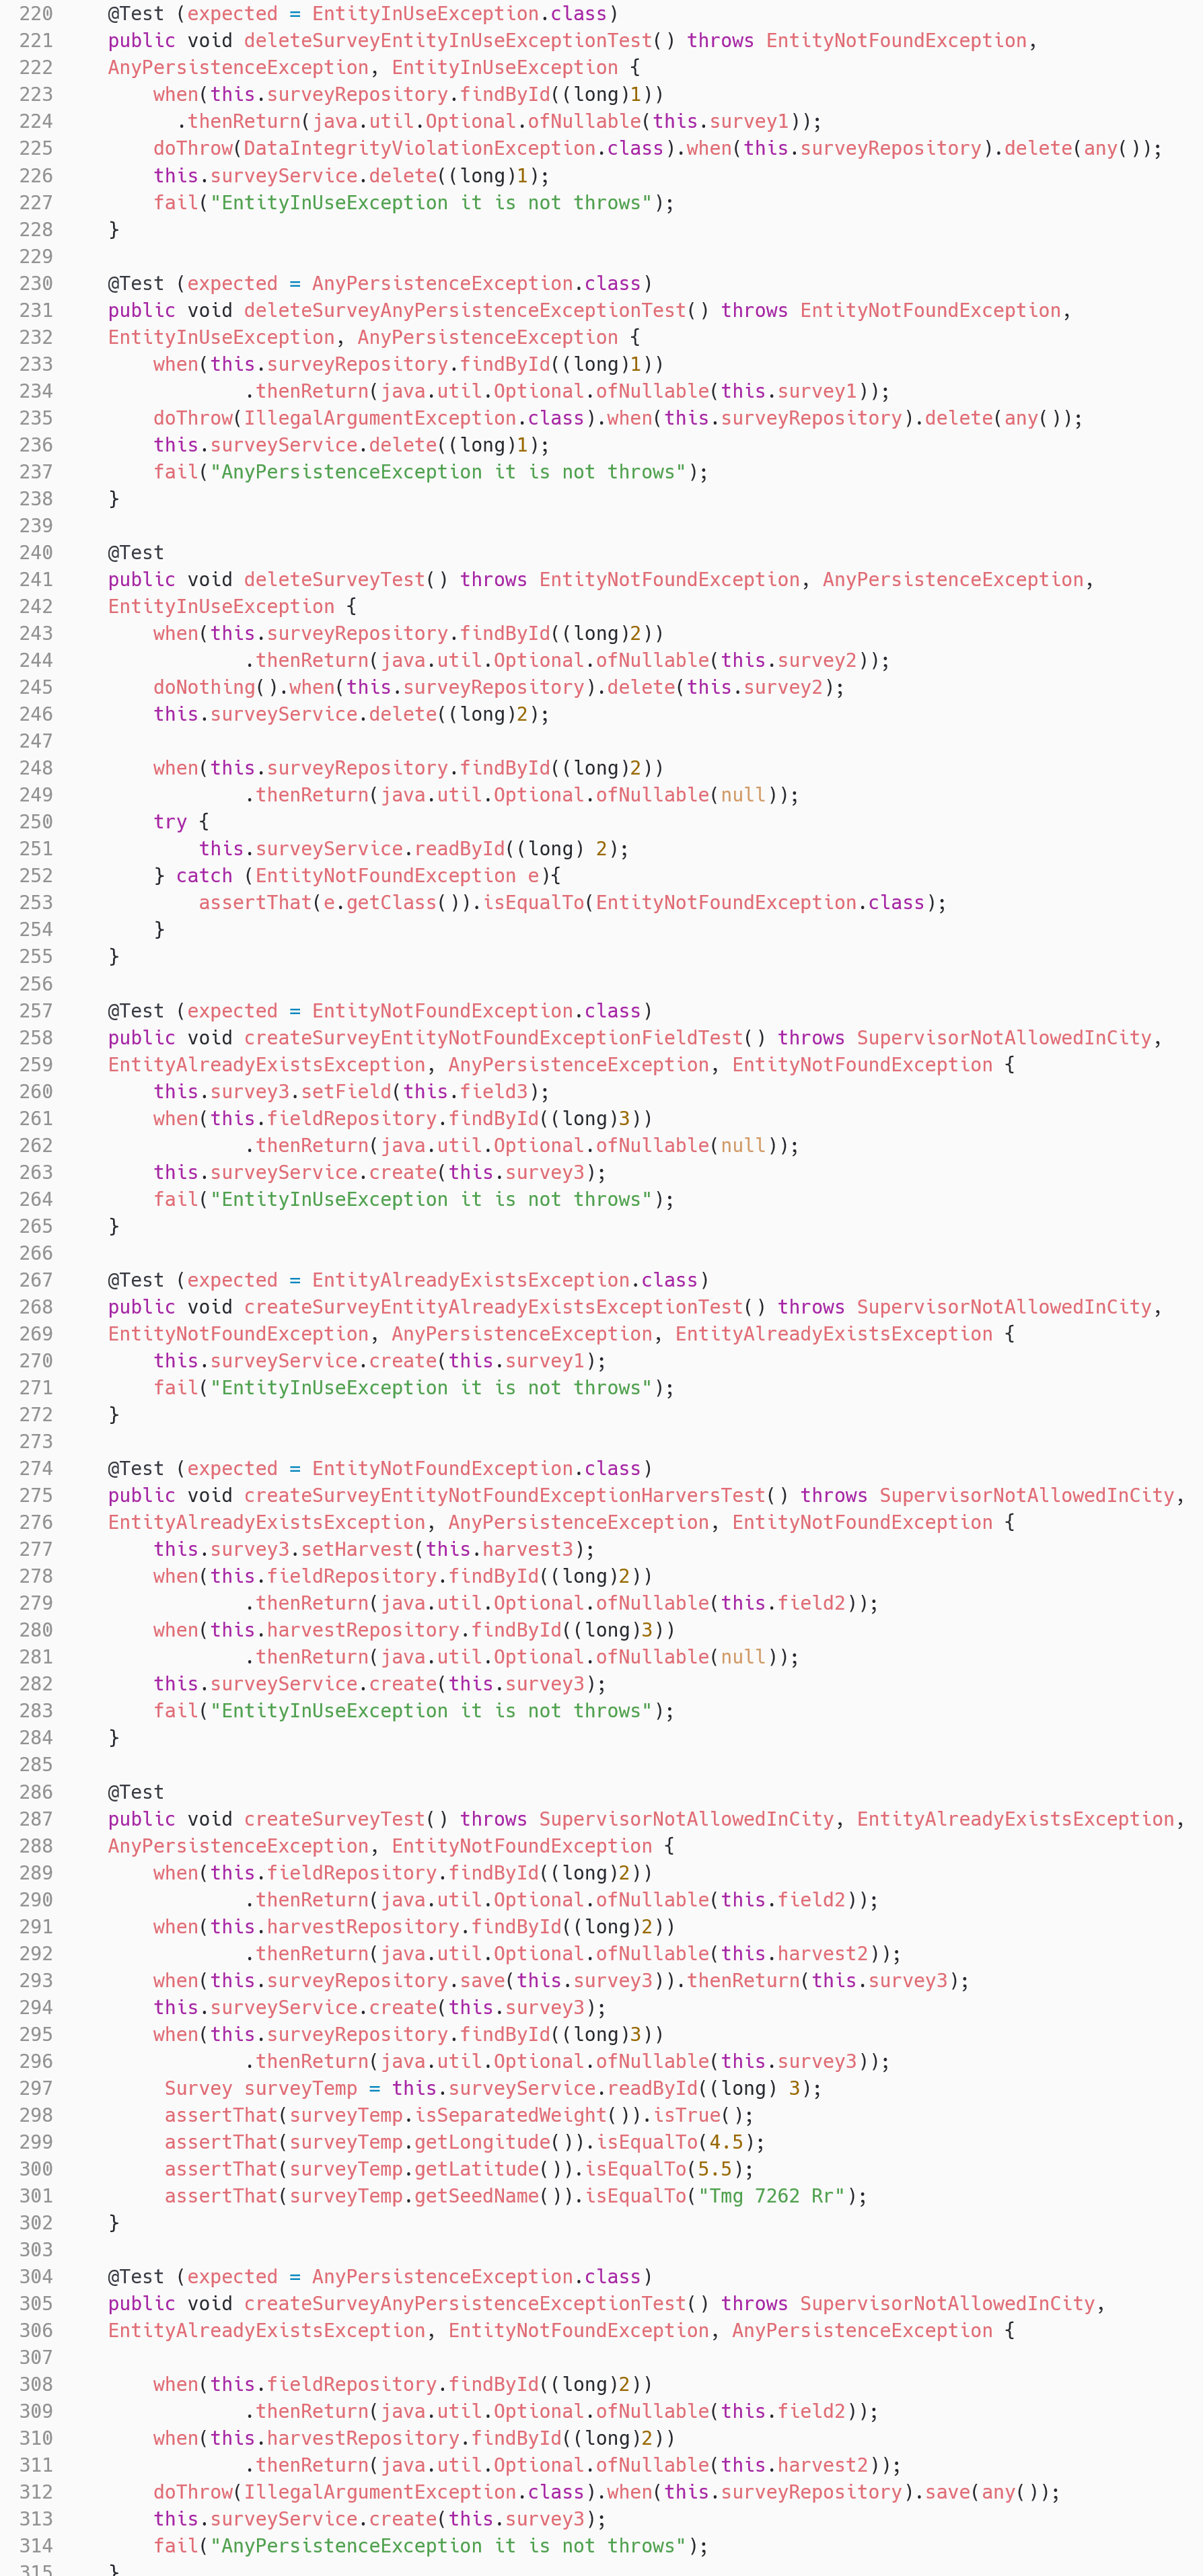
\includegraphics[scale=0.26]{dados/figuras/carbonSurveyService2.png}
\end{figure}

\begin{figure}[H]
	\centering
	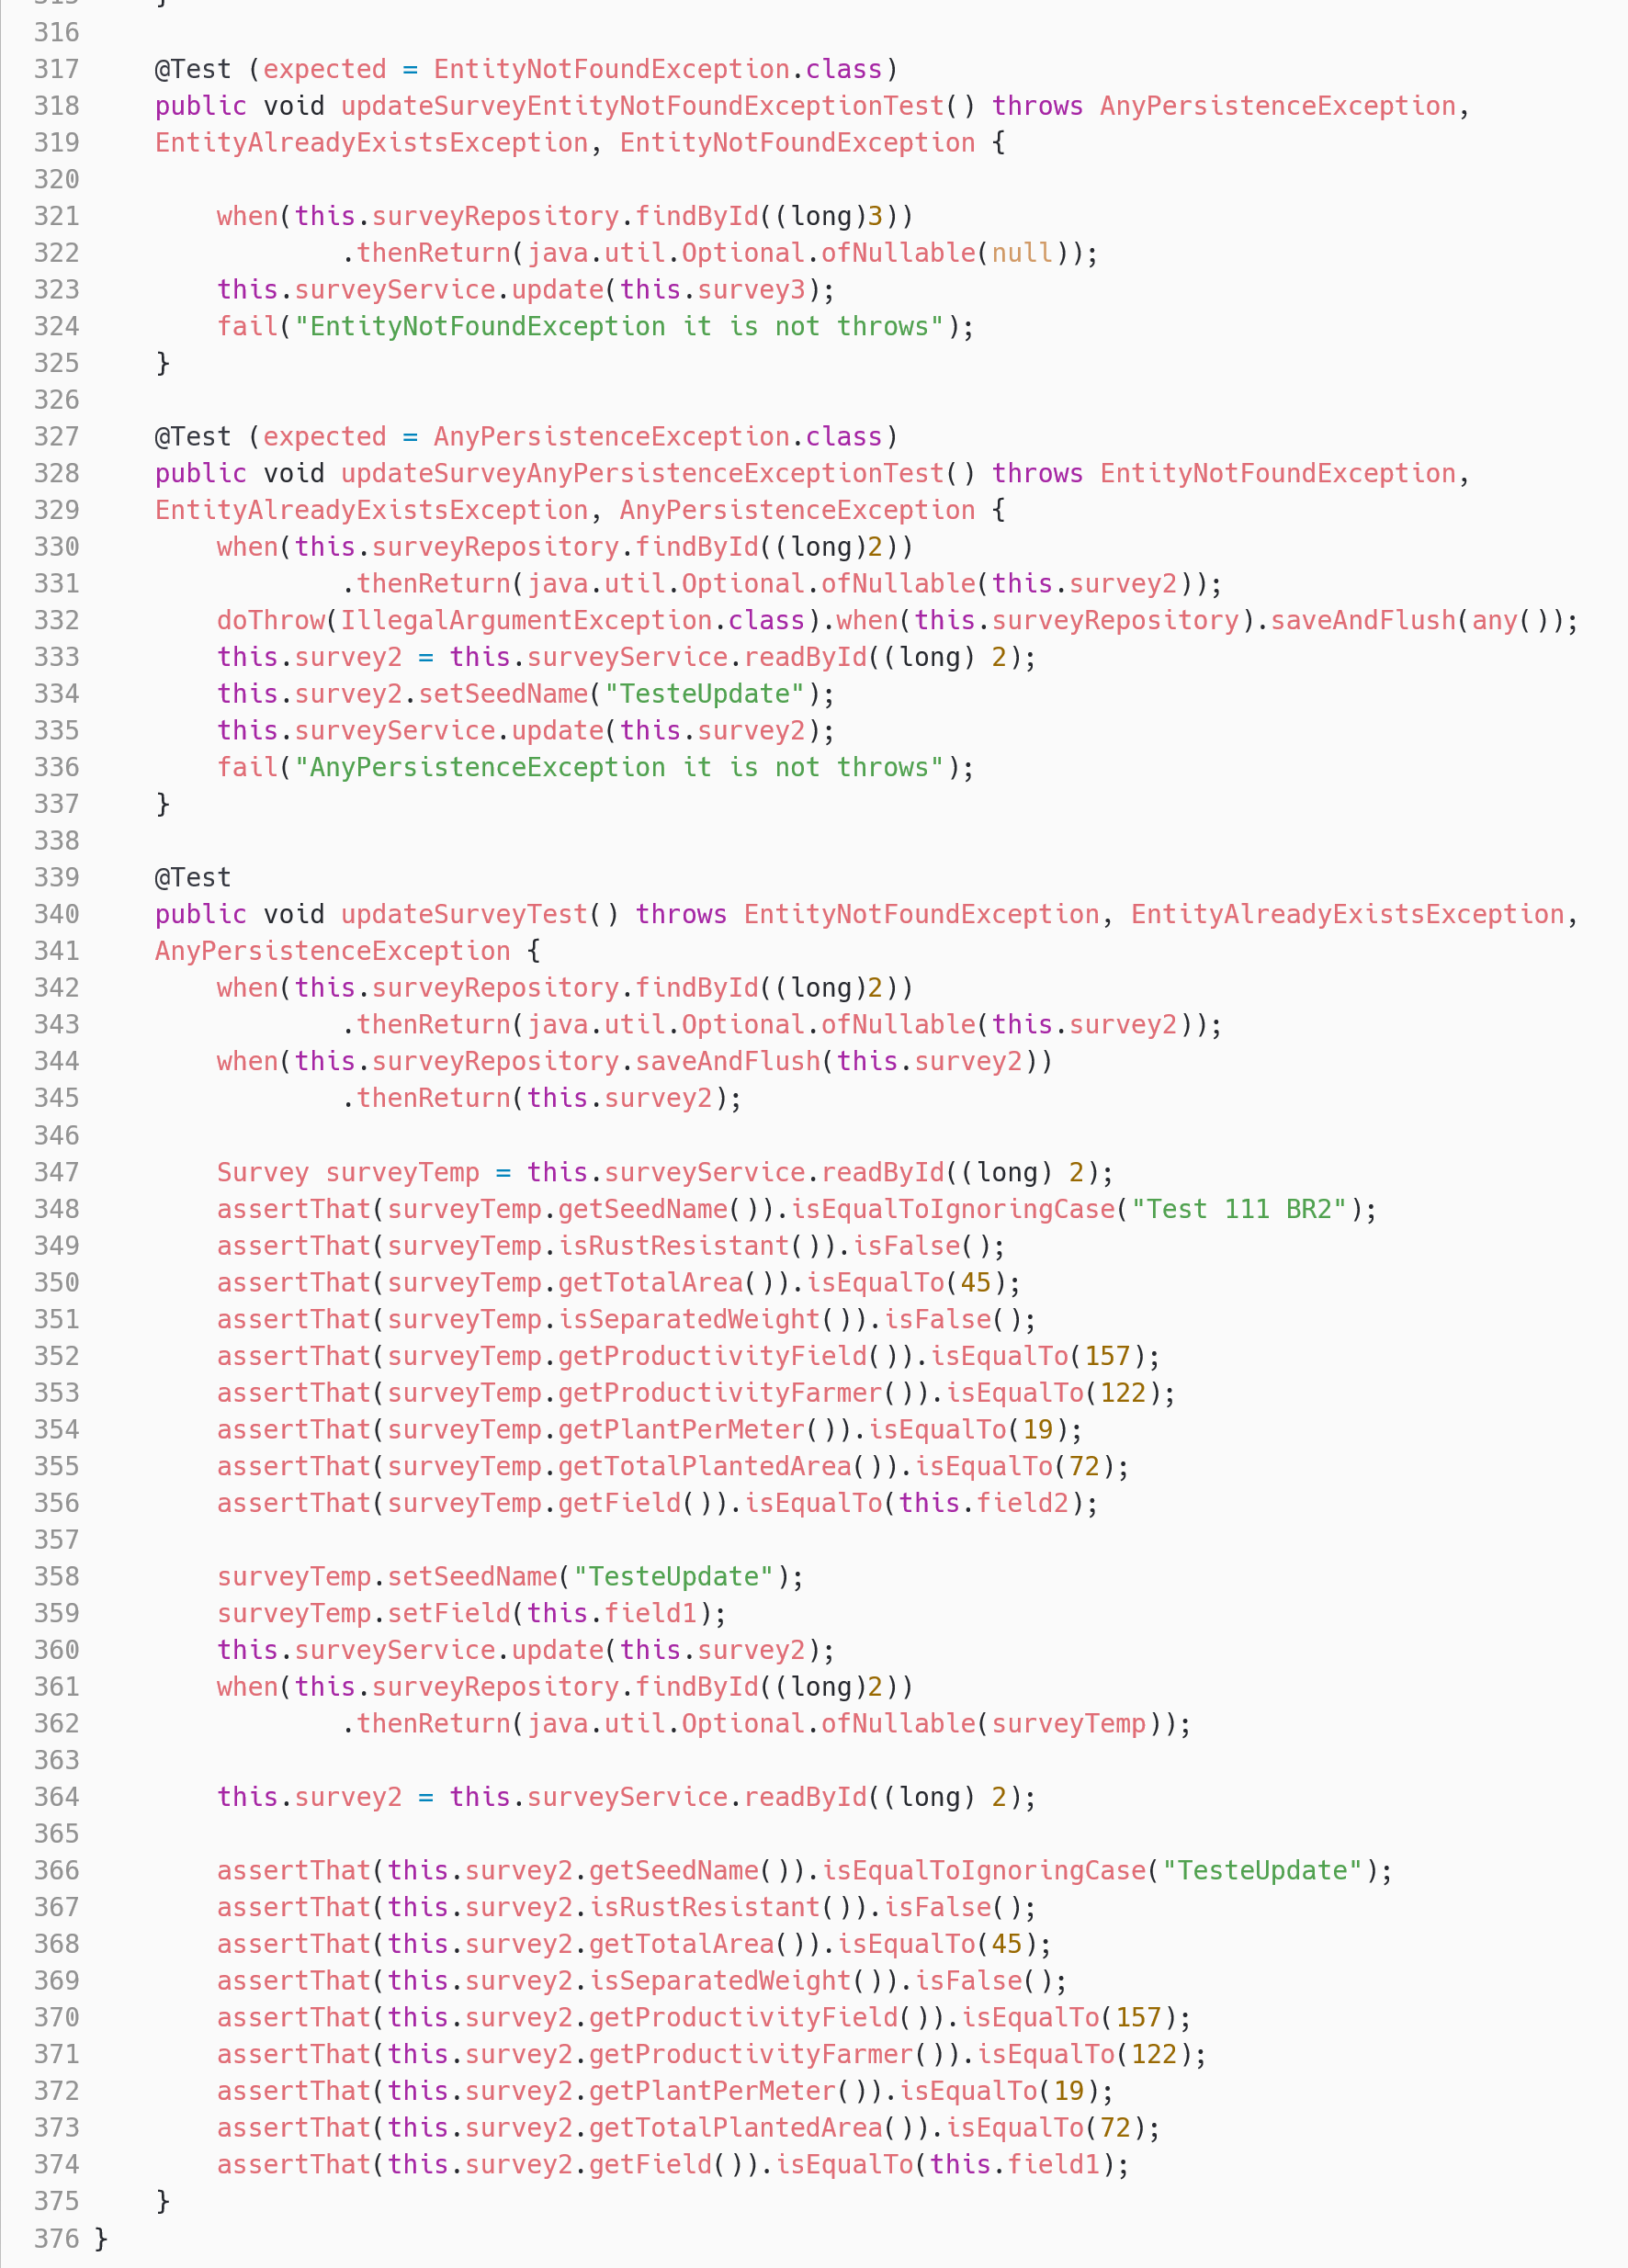
\includegraphics[scale=0.27]{dados/figuras/carbonSurveyService3.png}
	\caption{Classe de Teste  SurveyServiceTest.java.}
	\label{testeSurveyService}
\end{figure}

Método de teste \textit{ readByIdSurveyTest ()} linhas 117 a 123 figura \ref{testeSurveyService}: Este teste busca uma pesquisa na base de dados pelo seu identificador único. A entrada consiste em um numeral do tipo \textit{“Long”}. A saída é um objeto do tipo \textit{“Survey”}. Nesta assertiva o método testado deve retornar o registro \textit{mocado} nas linhas 119 e 120, o qual corresponde ao objeto comparado.

Método de teste \textit{ readByIdSurveyEntityNotFoundExceptionTest ()} linhas 125 a 131 figura \ref{testeSurveyService}: Este teste busca um registro do tipo \textit{“Survey”} na base de dados pelo seu identificador único, quando não encontrado é gerada uma exceção. A entrada consiste em um numeral do tipo \textit{“Long”}. A saída é uma exceção do tipo \textit{“EntityNotFoundException”}. Nesta assertiva o método testado deve retornar uma exceção, ao buscar um objeto pelo índice passado como parâmetro, ao realizar a consulta no banco um registro vazio é retornado, o que é simulado nas linhas 127 e 128, o que garante o lançamento da exceção \textit{“EntityNotFoundException”}.

Método de teste \textit{ readFieldbyIdTest ()} linhas 133 a 139 figura \ref{testeSurveyService}: Este teste busca um registro do tipo \textit{Field} na base de dados pelo seu identificador único. A entrada consiste em um numeral do tipo \textit{“Long”}. A saída é um objeto do tipo \textit{Field}. Nesta assertiva o método testado deve retornar o objeto \textit{mocado} nas linhas 135 e 136, o qual corresponde ao objeto comparado.

Método de teste \textit{ readFieldbyIdEntityNotFoundExceptionTest ()} linhas 141 a 147 figura \ref{testeSurveyService}: Este teste busca um registro do tipo \textit{Field} na base de dados pelo seu identificador único, quando não encontrado é gerada uma exceção. A entrada consiste em um numeral do tipo \textit{“Long”}. A saída é uma exceção do tipo \textit{“EntityNotFoundException”}. Nesta assertiva o método testado deve retornar uma exceção, ao buscar um objeto pelo índice passado como parâmetro, ao realizar a consulta no banco um registro vazio é retornado, o que é simulado nas linhas 143 e 144, o que garante o lançamento da exceção \textit{“EntityNotFoundException”}.

Método de teste \textit{ readHarvestByIdTest ()} linhas 150 a 157 figura \ref{testeSurveyService}: Este teste busca um registro do tipo \textit{“Harvest”} na base de dados pelo seu identificador único. A entrada consiste em um numeral do tipo \textit{“Long”}. A saída é um objeto do tipo \textit{“Harvest”}. Nesta assertiva o método testado deve retornar o objeto \textit{mocado} nas linhas 152 e 153, o qual corresponde ao objeto comparado.

Método de teste \textit{ readHarvestByIdEntityNotFoundExceptionTest ()} linhas 159 a 165 figura \ref{testeSurveyService}: Este teste busca um registro do tipo \textit{“Harvest”} na base de dados pelo seu identificador único, quando não encontrado é gerada uma exceção. A entrada consiste em um numeral do tipo \textit{“Long”}. A saída é uma exceção do tipo \textit{“EntityNotFoundException”}. Nesta assertiva o método testado deve retornar uma exceção, ao buscar um objeto pelo índice passado como parâmetro, ao realizar a consulta no banco um registro vazio é retornado, o que é simulado nas linhas 161 e 161, o que garante o lançamento da exceção \textit{“EntityNotFoundException”}.

Método de teste \textit{ readAllFieldsTest ()} linhas 167 a 175 figura \ref{testeSurveyService}: Este teste busca os registros do tipo \textit{Field} na base de dados. Não há entrada de dados.  A saída é uma lista do tipo \textit{Field}. Nesta assertiva o método testado deve retornar a lista criada na linha 169, que contém dois registros correspondentes a comparação.

Método de teste \textit{ readAllHarvestsTest ()} linhas 177 a 185 figura \ref{testeSurveyService}:  Este teste busca os registros do tipo \textit{“Harvest”} na base de dados. Não há entrada de dados.  A saída é uma lista do tipo \textit{“Harvest”}. Nesta assertiva o método testado deve retornar a lista criada na linha 179, que contém dois registros correspondentes a comparação.

Método de teste \textit{ readAllFieldsOutOfCurrentHarvestTest ()} linhas 187 a 195 figura \ref{testeSurveyService}: Este teste busca os registros do tipo \textit{Field} na base de dados que pertencem a colheita. A entrada é um numeral do tipo \textit{“Long”} identificador único de uma colheita.  A saída é uma lista do tipo \textit{Field} contendo os registros que pertencem a colheita. Nesta assertiva o método testado deve retornar a lista criada na linha 189, que contém um registro correspondente a comparação.

Método de teste \textit{ readByHarvestIdTest ()} linhas 197 a 201 figura \ref{testeSurveyService}: Este teste lista todas as pesquisas do banco de dados que contém uma determinada colheita. A entrada é um numeral do tipo \textit{“Long”} identificador único de uma colheita. A Saída é uma lista do tipo \textit{“Survey”} contendo as pesquisas salvas na base de dados que contem a colheita. Nesta assertiva o método testado deve retornar a lista criada na linha 106, que contem 2 objetos do tipo \textit{survey} correspondentes a comparação.

Método de teste \textit{ readByHarvestIdEntityNotFoundExceptionTest ()} linhas 205 a 209 figura \ref{testeSurveyService}: Este teste lança uma exceção do tipo \textit{“EntityNotFoundException”} quando não encontra uma pesquisa que contenha a colheita. A entrada é um numeral do tipo \textit{“Long”} identificador único de uma colheita. A Saída é uma exceção do tipo \textit{“EntityNotFoundException”}. Nesta assertiva o método testado deve lançar uma exceção do tipo \textit{“EntityNotFoundException”}.

Método de teste \textit{ deleteSurveyEntityNotFoundExceptionTest ()} linhas 211 a 218 figura \ref{testeSurveyService}: Este teste consiste em deletar um registro do tipo \textit{“Survey”}, mas o item a ser deletado não existe na base de dados. A Entrada consiste em um objeto do tipo \textit{“Survey”}. A Saída é o lançamento da exceção \textit{“EntityNotFoundException”}. A assertiva tenta deletar um registro, mas ao consultar o registro na base de dados simulada pelas linhas 214 e 215 o retorno é um nulo pois ele não existe na base, há o lançamento da exceção.  

Método de teste \textit{ deleteSurveyEntityInUseExceptionTest ()} linhas 220 a 228 figura \ref{testeSurveyService}: Este teste consiste em deletar um registro do tipo \textit{“Survey”}, mas o item a ser deletado está sendo utilizado na base de dados. A Entrada consiste em um objeto do tipo \textit{“Survey”}. A Saída é o lançamento da exceção \textit{“UseEntityInUseException”}. A assertiva tenta deletar um registro, mas este está sendo utilizado na base de dados simulada pela linha 225, há o lançamento da exceção.  

Método de teste \textit{ deleteSurveyAnyPersistenceExceptionTest ()} linhas 230 a 238 figura \ref{testeSurveyService}: Este teste consiste em deletar um registro do tipo \textit{“Survey”}, mas o item a ser deletado gera um erro na base de dados. A Entrada consiste em um objeto do tipo \textit{“Survey”}. A Saída é o lançamento da exceção \textit{“AnyPersistenceException”}. A assertiva tenta deletar um registro, mas um erro é gerado, há o lançamento da exceção.

Método de teste \textit{ deleteSurveyTest ()} linhas 240 a 255 figura \ref{testeSurveyService}: Este teste consiste em deletar um registro do tipo \textit{“Survey”}. A Entrada consiste em um objeto do tipo \textit{“Survey”}. Não há saída de dados.  A assertiva deleta um registro do banco linha 245, a validação é feita ao tentar consultar este registro no banco simulado e o retorno é uma exceção do tipo \textit{“EntityNotFoundException”}.  

Método de teste \textit{ createSurveyEntityNotFoundExceptionFieldTest ()} linhas 257 a 265 figura \ref{testeSurveyService}: Este teste consiste em criar um registro do tipo \textit{“Survey”}, mas o item a ser atualizado não possui um \textit{Field}. A Entrada consiste em um objeto do tipo \textit{“Survey”}. A Saída é o lançamento da exceção \textit{“EntityNotFoundException”}. A assertiva tenta criar um registro, mas ao buscar um registro do tipo \textit{Field} na base de dados simulada pela linha 261 o retorno é um nulo pois ele não existe na base, há o lançamento da exceção.  

Método de teste \textit{ createSurveyEntityAlreadyExistsExceptionTest ()} linhas 267 a 272 figura \ref{testeSurveyService}: Este teste consiste em tentar criar um novo registro do tipo \textit{“Survey”}, mas o item a ser criado é identificado como já existente na base de dados. A Entrada consiste em um objeto do tipo \textit{“Survey”}. A Saída é o lançamento da exceção \textit{“EntityAlreadyExistsException”}. A assertiva tenta inserir um registro que já se encontra na base de dados simulada pela linha 106, o que proporciona o lançamento da exceção.  

Método de teste \textit{ createSurveyEntityNotFoundExceptionHarversTest ()} linhas 274 a 284 figura \ref{testeSurveyService}: Este teste consiste em criar um registro do tipo \textit{“Survey”}, mas o item a ser atualizado não possui uma colheita. A Entrada consiste em um objeto do tipo \textit{“Survey”}. A Saída é o lançamento da exceção \textit{“EntityNotFoundException”}. A assertiva tenta atualizar um registro, mas ao buscar um registro do tipo \textit{“Harvest”} na base de dados simulada pela linha 280 o retorno é um nulo pois ele não existe na base, há o lançamento da exceção.  

Método de teste \textit{ createSurveyTest ()} linhas 286 a 302 figura \ref{testeSurveyService}: Este teste consiste em criar um novo registro do tipo \textit{“Survey”} na base de dados. A Entrada consiste em um objeto do tipo \textit{“Survey”}. O método não gera uma saída. A validação é feita através de um \textit{try cath}, que captura qualquer exceção que ocorra ao salvar o objeto. Como o método não lança uma exceção ele é aceito. A assertiva, no entanto, é feita através do repositório \textit{mocado} linhas 295 e 296, depois de inserido é simulada uma consulta pelo identificador único do objeto inserido o qual deve retornar o objeto que acaba de ser inserido.

Método de teste \textit{ createSurveyAnyPersistenceExceptionTest ()} linhas 304 a 315 figura \ref{testeSurveyService}: Este teste consiste em tentar criar um novo registro do tipo \textit{“Survey”}, mas o item a ser criado gera algum erro na base de dados. A Entrada consiste em um objeto do tipo \textit{“Survey”}. A Saída é o lançamento da exceção \textit{“AnyPersistenceException”}. A assertiva tenta inserir um registro na base de dados simulada pela linha 312, o que proporciona o lançamento da exceção.

Método de teste \textit{ updateSurveyEntityNotFoundExceptionTest ()} linhas 317 a 325 figura \ref{testeSurveyService}: Este teste consiste em atualizar um registro do tipo \textit{“Survey”}, mas o item a ser atualizado não existe na base de dados. A Entrada consiste em um objeto do tipo \textit{“Survey”}. A Saída é o lançamento da exceção \textit{“EntityNotFoundException”}. A assertiva tenta atualizar um registro, mas ao consultar o registro na base de dados simulada pela linha 321 o retorno é um nulo pois ele não existe na base, há o lançamento da exceção.  

Método de teste \textit{ updateSurveyAnyPersistenceExceptionTest ()} linhas 327 a 337 figura \ref{testeSurveyService}: Este teste consiste em atualizar um registro do tipo \textit{“Survey”}, mas o item a ser alterado gera um erro na base de dados. A Entrada consiste em um objeto do tipo \textit{“Survey”}. A Saída é o lançamento da exceção \textit{“AnyPersistenceException”}. A assertiva tenta atualizar um registro, mas ao alterar a base de dados simulada pela linha 332 o retorno é um exceção, há o lançamento da exceção.

Método de teste \textit{ updateSurveyTest ()} linhas 339 a 375 figura \ref{testeSurveyService}: Este teste consiste em atualizar um registro do tipo \textit{“Survey”}. A Entrada consiste em um objeto do tipo \textit{“Survey”}. Não há saída de dados. As assertivas consistem em recuperar um objeto da base de dados simulada linha 342, atualizar os campos deste objeto linhas 358 e 359, e em seguida atualizar esse registro na base linha 344. Caso não haja o lançamento de uma exceção o objeto atualizado é recuperado da base simulada, linha 361, e em seguida é feita as assertivas dos dados atualizados.

Após a execução dos testes a cobertura das entradas e saídas de dados da classe \textit{SurveyService}.java é de 100\%.



\subsection{RESULTADO GERAL DOS TESTES PACOTE SERVICE}

Para alcançar a cobertura de 100\% de todos os métodos linhas e classes do pacote Service foram criados no total 294 testes de unidade, onde 283 foram aprovados, 5 ignorados e 6 rejeitado. Cada classe possui o seguinte número de casos de teste: 

\begin{itemize}
        \item Pacote Base:
\begin{itemize}
    \item Classe \textit{FieldServiceTest}: 23 casos de teste aprovados;
    \item Classe \textit{RegionServiceTest}: 18 casos de teste aprovados, 1 reprovado;
    \item Classe \textit{FarmerServiceTest}: 12 casos de teste aprovados, 2 reprovados;
    \item Classe \textit{LocalDateTimeConverterTest}: 2 casos de teste aprovados;
    \item Classe \textit{MacroRegionServiceTest}: 12 casos de teste aprovados, 2 reprovados;
    \item Classe \textit{CityServiceTest}: 3 casos de teste aprovados;
    \item Classe \textit{SupervisorServiceTest}: 16 casos de teste aprovados, 1 reprovado;
\end{itemize}
  \item Pacote MIP:
  \begin{itemize} 
    \item Classe \textit{PestDiseaseServiceTest}: 14 casos de teste aprovados;
    \item Classe \textit{PestNaturalPredatorServiceTest}: 14 casos de teste aprovados; 
    \item Classe \textit{PestServiceTest}: 14 casos de teste aprovados;
    \item Classe \textit{MIPSampleServiceTest}: 18 casos de teste aprovados, 1 ignorado;
\end{itemize}
  \item Pacote \textit{Survey}:
  \begin{itemize}   
    \item Classe \textit{SurveyServiceTest}: 23 casos de teste aprovados, 1 ignorado;
    \item Classe \textit{HarvestServiceTest}: 14 casos de teste aprovados;
\end{itemize}
  \item Pacote MID:
  \begin{itemize}
    \item Classe \textit{BladeReadingResponsibleEntityServiceTest}: 18 casos de teste aprovados;
    \item Classe \textit{MIDRustSampleServiceTest}: 13 casos de teste aprovados;
    \item Classe \textit{BladeReadingResponsiblePersonServiceTest}: 18 casos de teste aprovados;
    \end{itemize}
    \item Pacote \textit{Pulverisation}:
  \begin{itemize}
    \item Classe \textit{ProductServiceTest}: 17 casos de teste aprovados, 1 ignorado;
    \item Classe \textit{PulverisationOperationServiceTest}: 20 casos de teste aprovados, 1 ignorado;
    \item Classe \textit{TargetServiceTest}: 14 casos de teste aprovados, 1 ignorado;
    \end{itemize}
    \end{itemize}



Como já dito anterior mente os testes podem garantir que o software é livre de defeitos mais, mas seu objetivo principal é revelar a presença de defeitos. Após a execução dos testes a taxa de cobertura foi de: 100\% das classes, 100\% dos métodos e 98\% das linhas. Como alguns casos de testes falharam não foi possível a cobertura de 100\% das linhas.


\section{TESTE IGNORADOS E REPROVADOS}

Em resumo, foram produzidos 652 testes de unidade, buscando a cobertura de 100\% das linhas, variáveis e métodos dos pacotes\textit{Entity}e Service do aplicativo MIP. Dentre eles 640 foram aprovados o equivalente a 98,16\% dos testes, 5 testes equivalente a 0,77\% foram ignorados e 7 falharam o que corresponde a 1,07\%.

\subsection{REPROVADOS}

Dos testes 7 casos falharam, os casos falhos e os motivos pelo qual falharam são listados a seguir:

  \begin{itemize}
    \item Pacote\textit{Entity}sub pacote \textit{base} classe \textit{Field}: O caso de teste \textit{“fieldTestAddSupervisorIsNull”} responsável por testar o método \textit{“field.addSupervisor(null)”} que recebe um nulo. O grande problema se deve na hora de fazer a listagem dos supervisores, ao percorrer a lista uma exceção do tipo \textit{“NullPointerException”} é lançada;

  \item Pacote \textit{Service} sub pacote \textit{base} classe \textit{FarmerServiceTest}: O caso de teste \textit{“updateFarmerServiceAnyPersistenceExceptionTest”}  responsável por testar o método \textit{“farmerService.update(Farmer)”} que atualiza um registro do tipo \textit{“Farmer”} deveria gerar uma exceção de persistência no banco de dados   ao tentar atualizar o registro, mas a exceção lançada é do tipo \textit{“EntityAlreadyExistsException”}. Antes da atualização o método de update recupera todos os registros do banco e verifica se o registro que será atualizado existe na lista, o que gera o lançamento da exceção pois o registro a ser atualizado não foi removido da lista;

  \item Pacote \textit{Service} sub pacote \textit{base} classe \textit{FarmerServiceTest}: O caso de teste \textit{“updateFarmerServiceTest”}  responsável por testar o método \textit{“farmerService.update(Farmer)”} que atualiza um registro do tipo \textit{“Farmer”} deveria atualizar o registro no banco de dados, mas é lançada uma exceção do tipo \textit{“EntityAlreadyExistsException”}. Antes da atualização o método de update recupera todos os registros do banco e verifica se o registro que será atualizado existe na lista, o que gera o lançamento da exceção pois o registro a ser atualizado não foi removido da lista;

  \item Pacote \textit{Service} sub pacote base classe \textit{MacroRegionServiceTest}: O caso de teste \textit{“updateMacroRegionServiceTest”  }responsável por testar o método \textit{“macroRegionService.update
  (macroRegion)”} que atualiza um registro do tipo \textit{“Macroregion” }deveria atualizar o registro no banco de dados, mas é lançada uma exceção do tipo \textit{“EntityAlreadyExistsException”}. Antes da atualização o método de update recupera todos os registros do banco e verifica se o registro que será atualizado existe na lista, o que gera o lançamento da exceção pois o registro a ser atualizado não foi removido da lista;

  \item Pacote \textit{Service} sub pacote base classe \textit{MacroRegionServiceTest: }O caso de teste \textit{“updateMacroRegionServiceAnyPersistenceExceptionTest”  }responsável por testar o método “macroRegionService.update(macroRegion)” que atualiza um registro do tipo\textit{ “Macroregion” }deveria gerar uma exceção de persistência no banco de dados   ao tentar atualizar o registro, mas a exceção lançada é do tipo \textit{“EntityAlreadyExistsException”}. Antes da atualização o método de update recupera todos os registros do banco e verifica se o registro que será atualizado existe na lista, o que gera o lançamento da exceção pois o registro a ser atualizado não foi removido da lista;

 \item Pacote \textit{Service} sub pacote \textit{base} classe \textit{RegionServiceTest}: O caso de teste\textit{ “readMacroRegionByIdRegionServiceEntityNotFoundExceptionTest”}  responsável por testar o método\textit{ “regionService.readMacroRegionById((long) 4)”} que busca um registro do tipo “MacroRegion” no banco de dados pelo identificador único gera uma exceção do tipo \textit{“NullPointerException”}. Quando o índice procurado não é encontrado há o lançamento de uma exceção do tipo \textit{“EntityNotFoundException”} a classe \textit{“RegionService”} faz o tratamento, retornando um objeto do tipo \textit{“MacroRegion”} vazio, mas ao utilizar o padrão \textit{Build} para a construção do objeto sem passar nenhum parâmetro o atributo nome que é do tipo \textit{string} é definido como \textit{null}, o que gera o lançamento da exceção na classe \textit{“MacroRegion” }no método \textit{“setName()”};

\item Pacote \textit{Service} sub pacote \textit{base} classe \textit{SupervisorServiceTest}: O caso de teste\textit{ “readRegionByIdSupervisorServiceEntityNotFoundExceptionTest”}  responsável por testar o método \textit{“supervisorService.readRegionById((long) 112)”} que busca um registro do tipo \textit{“Region” }no banco de dados pelo identificador único gera uma exceção do tipo\textit{ “NullPointerException”}. Quando o índice procurado não é encontrado há o lançamento de uma exceção do tipo \textit{“EntityNotFoundException”} a classe \textit{“SupervisorService” }faz o tratamento, retornando um objeto do tipo \textit{“Region” }vazio, mas ao utilizar o padrão \textit{Build} para a construção do objeto sem passar nenhum parâmetro o atributo nome que é do tipo \textit{string} é definido como \textit{null}, o que gera o lançamento da exceção na classe \textit{“Region”} no método \textit{“setName()”;}

    \end{itemize}



\subsection{IGNORADOS}

Foram ignorados 5 casos de testes, os casos ignorados e os motivos pelo qual foram ignorados são listados a seguir:
  \begin{itemize}
    \item Pacote \textit{Service} sub pacote mip classe \textit{MIPSampleServiceTest}: O teste \textit{“createSupervisorNotAllowedInCityTest}” foi ignorado pois o método testado “\textit{mipSampleService.create(new mipSampleTest)”} nuca lança a exceção \textit{“SupervisorNotAllowedInCity”};
    
\item Pacote \textit{Service} sub pacote survey classe SurveyServiceTest: O teste \textit{“readByHarvestIdEntityNotFoundExceptionTest”} foi ignorado pois o método testado \textit{“surveyService
.readByHarvestId(this.harvest3.getId())”} nuca lança a exceção \textit{“EntityNotFoundException”} mas retorna uma lista vazia;

\item Pacote \textit{Service} sub pacote \textit{pulverisation} classe \textit{PulverisationOperationServiceTest}: O teste “createPulverisationOperationServiceEntityNotFoundExceptionTest” foi ignorado pois o método testado “pulverisationOperationService.create(new pulverisationOperation)” nuca lança a exceção \textit{“EntityNotFoundException”};

\item Pacote \textit{Service} sub pacote \textit{pulverisation} classe \textit{ProductServiceTest}: O teste\textit{ “createProductServiceEntityNotFoundExceptionTest”} foi ignorado pois o método testado\textit{ “productService.create(new product)”} nuca lança a exceção \textit{“EntityNotFoundException”};

\item Pacote \textit{Service} sub pacote \textit{pulverisation} classe \textit{TargetServiceTest}: O teste “\textit{createTargetServiceEntityNotFoundExceptionTest}” foi ignorado pois o método testado “\textit{targetService.create(new target3)}” nuca lança a exceção \textit{“EntityNotFoundException”};


    \end{itemize}
